\documentclass[english, GINF]{TFGEPSUIB}

\usepackage[printonlyused]{acronym}
\usepackage{siunitx}
\usepackage[draft=false, backref, hyperindex, plainpages=false, breaklinks=true, bookmarksnumbered=true]{hyperref}

\usepackage{paralist} %% Compact list environments
\usepackage{amsmath}  %% Mathematics
\usepackage{amsthm}
\usepackage{amsfonts}
\usepackage{url}      %% Hyperlinks
\usepackage{listings} %% Source code highlighting
\usepackage{graphicx}
\usepackage{listings}
\usepackage{xcolor}
\usepackage{hhline}
\usepackage{siunitx}
\usepackage[most]{tcolorbox}
\usepackage{geometry}
\usepackage{adjustbox}
\usepackage{tcolorbox}
\usepackage{multirow, tabularx}
\usepackage{booktabs}
\usepackage{multirow}
\usepackage{longtable}
\usepackage{gensymb}
\usepackage{multicol}
\usepackage{float}

\estudis{\MakeUppercase{Master degree}}

% Thesis info
\title{Device for Movement Analysis Using Inertial Sensors}
\author{\MakeUppercase{Bedřich Said}}
\tutor{Dr. Antoni Jaume i Capó}
\supervisor{RNDr. Zdeněk Matěj, Ph.D.}
\date{May 22, 2018}

\bibliographystyle{url}

\theoremstyle{definition}
\newtheorem{definition}{Definition}[section]

\theoremstyle{remark}
\newtheorem*{remark}{Remark}

%% Special colors definitions
\definecolor{background}{HTML}{F5DD9D}
\definecolor{symbolColorTop}{HTML}{FFECB3}
\definecolor{symbolColorBox}{HTML}{FFF9E5}
\definecolor{gray}{rgb}{0.25,0.25,0.25}
\definecolor{darkblue}{rgb}{0.0,0.0,0.6}
\definecolor{cyan}{rgb}{0.0,0.6,0.6}
\definecolor{lightblue}{rgb}{0.9,0.95,1.0}
\definecolor{darkgreen}{rgb}{0.0,0.6,0.0}
\definecolor{brown}{HTML}{A52A2A}
\definecolor{darkmagenta}{HTML}{8B008B}

\lstset{
	basicstyle      = \ttfamily,%
	identifierstyle = \color{black},%
	keywordstyle    = \color{blue},%
	keywordstyle    = {[2]\color{cyan}},%
	keywordstyle    = {[3]\color{olive}},%
	stringstyle     = \color{teal},%
	commentstyle    = \itshape\color{magenta}}

\newcommand\Cpp{
	\lstset{
		basicstyle=\ttfamily,
		columns=fullflexible,
		showstringspaces=false,
		tabsize=4,
		numbers=left,
		xleftmargin=2em,
		backgroundcolor = \color{lightblue},
		language=C++,
		identifierstyle=\color{brown},
		keywordstyle=\color{blue},
		stringstyle=\color{red},
		commentstyle=\color{darkgreen},
		morecomment=[l][\color{darkmagenta}]{\#}
	}
}

%% Table colors
\newcommand\greenLow[0]{\cellcolor{green!25} Low}
\newcommand\greenSpare[0]{\cellcolor{green!25} Spare}
\newcommand\yellowMedium[0]{\cellcolor{yellow!25} Medium}
\newcommand\redHigh[0]{\cellcolor{red!25} High}

\newcommand\greenYes[0]{\cellcolor{green!25} Yes}
\newcommand\redNo[0]{\cellcolor{red!25} No}

\newcommand\greenCell[1]{\cellcolor{green!25} #1}
\newcommand\yellowCell[1]{\cellcolor{yellow!25} #1}
\newcommand\redCell[1]{\cellcolor{red!25} #1}

%% Definition of the box with declarations of used symbols.
\newcommand\highlightedBox[2]{
	\tcbset{
		enhanced,
		colback=symbolColorBox,
		boxrule=1.0pt,
		colframe=symbolColorTop!80!black,
		coltitle=black,
		fonttitle=\bfseries
	}
	\vspace{0.5cm}
	\begin{tcolorbox}[title=#1:,lifted shadow={0mm}{0mm}{0mm}{0.1mm}{black!50!white}]
		#2
	\end{tcolorbox}
	\vspace{0.5cm}
}

\newcommand\itwoc[0]{
	I$^{2}$C
}

\newcommand\ind[1]{#1\index{#1}}

\begin{document}
\tcbset{tab2/.style={enhanced,fonttitle=\bfseries,fontupper=\normalsize\sffamily, colback=yellow!10!white, colframe=black, colbacktitle=white, coltitle=black, center title}}

%\portada
\frontmatter

\cleartorecto \tableofcontents

%!TeX root=indexUIB.tex
\chapter{Acronyms}

\begin{acronym}

\acro{PCB}[PCB]{Printed Circuit Board}
\acro{CGI}[CGI]{Computer Generated Imagery}
\acro{IMU}[IMU]{Inertial Measurement Unit}
\acro{SMT}[SMT]{Surface Mount Technology}
\acro{SMD}[SMD]{Surface Mounted Device}
\acro{BOM}[BOM]{Bill of Materials}
\acro{EAGLE}[EAGLE]{Easy Applicable Graphical Layout Editor}
\acro{TDOA}[TDOA]{Time Difference of Arrival}
\acro{HAL}[HAL]{Hardware Abstraction Layer}
\acro{JTAG}[JTAG]{Joint Test Action Group (standard)}
\acro{SWD}[SWD]{Serial Wire Debug (interface)}
\acro{ESP-IDF}[ESP-IDF]{Espressif IoT Development Framework}
\acro{POSIX}[POSIX]{Portable Operating System Interface}
\acro{API}[API]{Application Programming Interface}
\acro{AHRS}[AHRS]{Attitude and Heading Reference System}
\acro{IoT}[IoT]{Internet of Things}
\acro{TCP}[TCP]{Transmission Control Protocol}

\end{acronym}

%!TeX root=indexUIB.tex

\chapter{Abstract}
Attitude sensors are more and more widely used and their price is decreasing. We can find them in many electronic systems designed for specific purposes. Some examples are in wearable devices, navigation or control systems. We can use some of the devices for covering new use cases and developing new systems. I still didn't find any device that fulfills all my requirements for developing new data processing algorithms.

I have developed a new wearable independent device for capturing and processing the measured data. The independence means no external wires and no external power supply here. The device is able to work outdoors, to log the measured data and to provide a direct output based on internal computations. The user can choose between completely wireless communication or wired connection to other electronics. The sensors measure inertial, attitude, position and atmospheric values.

For outdoor testing of the device, I selected a task about movement analysis of a horse. The devices were placed on the horse's body as wearable devices and I was developing algorithms for determination of the type of its movement -- stand, walk, trot or gallop. The algorithm first determines very basic types of movements and then it's looking for more advanced ones based on previous results. The types of movement are defined as statements, so new types of movement of any subject can be detected without modification of the computation code.

In general, the developed device can be used for sensor data capturing, onboard data processing, navigation or control of moving mechanics. The device works independently, so it is easy to install on the measured subjects.


\newgeometry{twoside, top=2.5cm, left=3cm, textwidth=15cm, textheight=24cm}
\mainmatter\pagestyle{ruled}

\chapter{Introduction}
//todo

\chapter{Hardware}
The hardware design is split into several steps in this paper. First, I had to decide if it's really necessary to build a new device or if I can find a suitable solution on the market. When we want to select a suitable device for our task, we have to know the specification of the task itself. The task is specified in section \ref{HWtaskAnalysis}. Based on the task we can specify all requirements that the selected device should meet (section \ref{HWrequirements}). Now, we can start looking for a device that fulfills all the requirements (section \ref{HWavailableSolutions}).

When we don't find any suitable device on the market, we can start to think about creating a new one. In my opinion, it's not a good way to start any development before doing the previous steps.

When we already start a development of a new hardware we can think about adding some additional requirements for increasing the versatility of the final hardware. Of course, the new requirements mustn't rapidly increase the final prize. But if the hardware will be used only in the specific task, it's usually unnecessary to add any other functionality. In this case, I'm adding some additional requirements in section \ref{HWadditionalRequirements}, because I think that in this case, I can add very high versatility with very low additional cost. The analysis of the final expenses is in section \ref{HWadditionalCosts}.

When I'm decided to develop a new hardware and I have the specification of all the requirements, I can start the development process. The selection of chips and other parts is in section \ref{HWdeviceSelection} and the printed circuit board (\ac{PCB}) design is discussed in section \ref{HWpcbDesign}.

Finally, the manufacturing of the first prototype is described in section \ref{HWmanufacturing}. With the first prototype, it's time for testing. The tests should find as many errors as possible and they should proof us if the requirements were already met. The section \ref{HWtesting}. The whole process is shown in the figure \ref{fig:HWprocess}.

\begin{figure}
	\centering
	\label{fig:HWprocess}
	\caption{Flowchart of the hardware design process}
	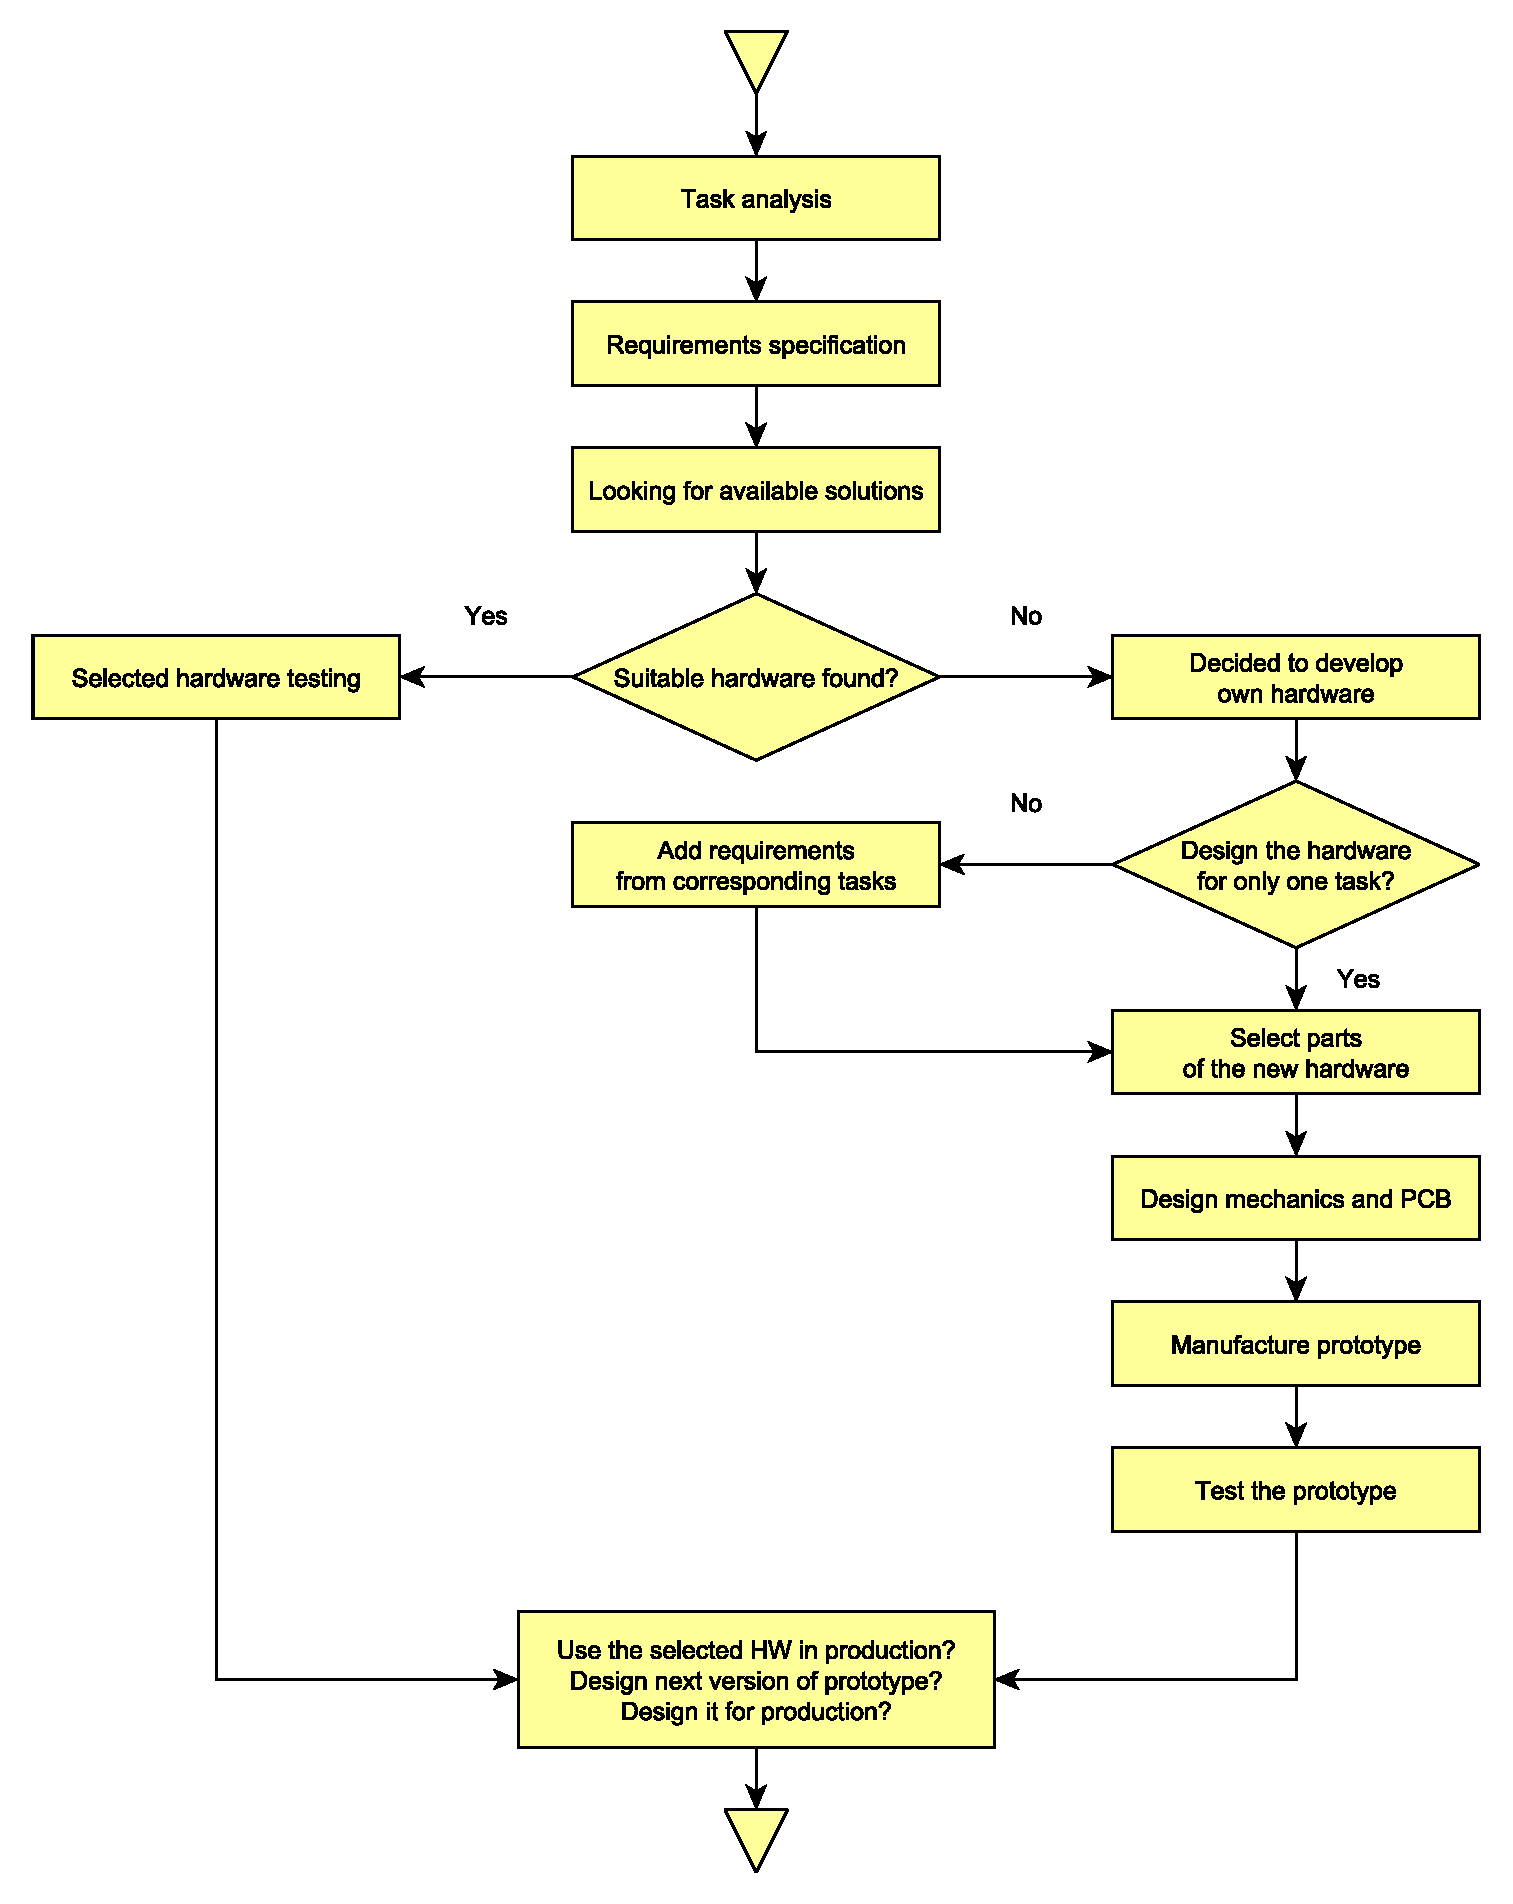
\includegraphics[width=\linewidth]{img/HWdesignProcess.pdf}
\end{figure}

\section{Task Analysis}
\label{HWtaskAnalysis}
When we define our complete task in the first step, then we can derive all requirements for our solution. Finally, we can check if our project was successful based on the previously defined task and requirements.

\highlightedBox{Movement analysis task description}{
	\begin{enumerate}
		\item Measuring of the movement of a subject
		\item Logging the measured data and sending them to post-processing
		\item Analysing of the movement and naming the specific categories of movements
	\end{enumerate}
}

The subject is an animal -- horse in this paper -- or human being or a moving machine. The post-processing can be done real-time during the measurement process, but this is not mandatory. The analysis is primarily focused to recognize known movements in logged data. For example, the categories of movement of a horse are stand, walk, trot, gallop, \dots

\section{Requirements}
\label{HWrequirements}
The development of a new hardware or software is usually driven by specified requirements. In this paper, I have specified two groups of requirements. The first group is based on the selected task to solve. The second group has lower priority and specifies all the requirements that I found during other similar tasks with similar hardware. The second group of requirements is adding higher versatility to the final electronic device with very low additional cost. These two groups of requirements are later merged and used as a source for next development of the hardware.

\subsection{High level requirements}

\paragraph{Measuring of the movement of a subject:} The solution should work outdoor. So, we cannot take into account any studio or laboratory-based technologies like Motion Capture (Mo-cap). On the other hand, we can replace the passive or active markers with the whole sensors and remove the necessary cameras. The sensor-based electronics is easier to install and can be used in large and complex areas. Based on this outdoor requirement I will consider only wearable sensor systems.

\paragraph{Logging the measured data and sending them to post-processing:} There are no wires acceptable for outdoor use, so we can log the data to internal memory or transmit them via any wireless technology. The wireless systems may be not fully reliable in complex areas with many objects. So, when we want to transmit the data directly it's still better to log them internally for later downloads.

\paragraph{Analysis of the movement and naming the specific categories of movements} This is a software requirement, so it's not very important during the hardware design. But this requirement defines what data we need to measure and this is a hardware requirement.

For the movement reconstruction, we primarily need data about position and attitude of every sensor. Some methods for movement classification don't need to know the exact location (for example accelerometer-based step counter). This task is focused on developing a new analysis of the movement, so now I cannot exactly say what sensors will be needed in the future. I can make a prediction that the inertial measurement unit (\ac{IMU}) and some location sensors will be needed. But there are some other sensors that produce interesting data according to the movement analysis, for example, a heart rate sensor according to animals.

Finally, I would like to add as many interesting sensors as possible, because it will give us more data sources and we are less limited by the data sources. The other advantage is multifunctionality of the hardware. On the other hand, these additional sensors should be added only into additional requirements with lower importance. Otherwise, the selection of an appropriate hardware (based on the requirements) will be manipulated by a number of probably unnecessary sensors.

\subsection{Low level requirements}
Finally, I've chosen a wearable sensors technology. The next requirements are specific to this technology and focused on the selection of the devices. Let's call a used wearable device or devices as Sensor Board. The table \ref{tab:requirements} shows the list of requirements for this Sensor Board.

\begin{table}
	\centering
	\caption{Sensor Board low level requirements 1}
	\label{tab:requirements}
	\begin{tcolorbox}[tab2,tabularx={X|p{12cm}},title=Importance legend]
		\greenLow    & Nice to have \\
		\yellowMedium & Very useful, reduce time or human effort \\
		\redHigh & Mandatory, impossible without this functionality \\
	\end{tcolorbox}
	\vspace{1cm}
	\begin{tcolorbox}[tab2,tabularx={|c|X|c|},title=Low level requirements 1]
		Category & Requirement & Importance \\ \hline \hline
		
		& Accumulator & \redHigh \\
		& Battery percentage indicator & \redHigh \\
		& Charging when external power applied & \redHigh \\
		& Voltage and current sensor & \yellowMedium \\
		& Power LED & \redHigh \\
		& Power switch & \redHigh \\
		& Automatic selection between external and battery power & \redHigh \\
		\multirow{-8}{*}{Power Supply} & Standardized charging connector & \yellowMedium \\ \hline
		
		& Accelerometer & \redHigh \\
		& Dynamic Gyroscope & \redHigh \\
		& Magnetometer & \redHigh \\
		& Indoor position & \yellowMedium \\
		& Outdoor position & \greenLow \\
		& Barometer & \greenLow \\
		\multirow{-7}{*}{Sensors} & Board temperature & \greenLow \\ \hline
		
		& Allow user programming & \redHigh \\
		& Wireless programming & \greenLow \\
		& Wired programming & \redHigh \\
		& Wireless & \redHigh \\
		& Standardized protocol & \redHigh \\
		& Wired access & \redHigh \\
		\multirow{-7}{*}{Communication} & Connector for external sensors & \greenLow \\ \hline
	\end{tcolorbox}
\end{table}

\begin{table}
	\centering
	\caption{Sensor Board low level requirements 2}
	\label{tab:requirements}
	\begin{tcolorbox}[tab2,tabularx={|c|X|c|},title=Low level requirements 2]
		Category & Requirement & Importance \\ \hline \hline
		
		& Logging all data for several hours & \redHigh \\
		& Sensor fusion coprocessor & \greenLow \\
		\multirow{-3}{*}{Functions} & LED indicators & \redHigh \\ \hline
		
		& Wearable design & \redHigh \\
		& Dimensions under \SI{6}{cm} & \redHigh \\
		& Dimensions under \SI{3}{cm} & \greenLow \\
		& Weight under \SI{50}{g} & \redHigh \\
		\multirow{-5}{*}{Mechanical} & Weight under \SI{20}{g} & \greenLow \\ \hline
		
		& Control multiple devices simultaneously & \yellowMedium \\
		& Download logged data & \redHigh \\
		& Streaming data during measurement & \yellowMedium \\
		& Start logging on multiple devices by clicking one button & \yellowMedium \\
		& Time synchronization of multiple devices & \redHigh \\
		\multirow{-6}{*}{Software} & Possibility to upload data to a server & \redHigh \\ 
	\end{tcolorbox}
\end{table}

\subsection{Additional requirements}
\label{HWadditionalRequirements}
The additional requirements are shown in table \ref{tab:additionalReq}.

\begin{table}
	\centering
	\label{tab:additionalReq}
	\caption{Additional requirements for the SensorBoard}
	\begin{tcolorbox}[tab2,tabularx={X|p{12cm}},title=Importance legend]
		\greenLow    & Nice to have \\ \hline
		\yellowMedium & Useful, can significantly improve functionality \\ \hline
		\st{\redHigh} & Not applicable \\ \hline
	\end{tcolorbox}
	\vspace{1cm}
	\begin{tcolorbox}[tab2,tabularx={|c|X|c|},title=Low level additional requirements]
		Category & Requirement & Importance \\ \hline \hline
		& Coprocessor for periodic computations like sensor fusion & \greenLow \\
		& Piezo buzzer & \greenLow \\
		\multirow{-3}{*}{Functions} & Buttons & \yellowMedium \\ \hline
		
		& Ambient light & \greenLow \\
		& Humidity & \greenLow \\
		& Sound (microphone) & \greenLow \\
		\multirow{-4}{*}{Sensors} & Ambient temperature & \greenLow \\ \hline
		
		& UART, I2C, SPI connector & \greenLow \\
		& PWM outputs & \greenLow \\
		\multirow{-3}{*}{Communication} & Analog inputs & \greenLow \\ \hline
		
		Software & NMEA input & \greenLow \\ \hline
	\end{tcolorbox}
\end{table}

\section{Available solutions}
\label{HWavailableSolutions}
The table \ref{tab:availableSolutions} shows the overview of existing devices I have found.

\begin{table}
	\centering
	\caption{Available solutions}
	\label{tab:availableSolutions}
	\begin{tcolorbox}[tab2,tabularx={|X|c|l|p{8cm}|},title=Available solutions]
		Device & Link & Price & Main disadvantages \\\hline\hline
		
		MetaWear        & \cite{MetaWear} & \$ 80  & Low memory, impossible longer logging. Loosing packets during streaming. \\
		ArduPilotMega   & \cite{APM26}    & \$ 250 & Dependent on external power supply, higher dimensions. \\
		pixHawk         & \cite{pixHawk}  & \$ 260 & Dependent on external power supply, higher dimensions. \\
		X-IMU           & \cite{XIMU}     & \$ 400 & Price. \\
		Smart Phone     & N/A             & \$ 100 & Impossible logging at higher frequencies, inaccurate logging frequency. \\
		Fitness sensors & N/A             & \$ 100 & Mostly closed commercial projects. \\
	\end{tcolorbox}
\end{table}

\section{Selection of parts for the new device}
\label{HWdeviceSelection}
Here I have finally decided to develop a new hardware. Now I'm looking for suitable parts for this new electronic device. The table \ref{tab:selectionParts} lists all the parts I took into account during the hardware development process.

\begin{table}
	\centering
	\caption{Selection of parts for the new electronic device}
	\label{tab:selectionParts}
	\begin{tcolorbox}[tab2,tabularx={|X|p{7cm}|c|c|},title=Available solutions]
		Part ID & Description & Datasheet & Selected \\\hline\hline
		TACTM-35N-F & Button & \cite{TACTM} & \greenYes \\
		ADP5062 & Power management and battery charger & \cite{analogdevices:ADP5062} & \greenYes \\
		ADP5063 & Power management and battery charger & \cite{analogdevices:ADP5063} & \redNo \\
		SI7006 & Humidity and temperature sensor & \cite{siliconlabs:SI7006} & \greenYes \\
		HDC2010YPAR & Humidity and temperature sensor & \cite{HDC2010YPAR} & \redNo \\
		SHTC1 & Humidity and temperature sensor & \cite{SHTC1} & \redNo \\
		DWM1000 & \ac{TDOA} location sensor (with antenna) & \cite{decawave:DWM1000} & \greenYes \\
		DW1000 & \ac{TDOA} location sensor (only sensor) & \cite{decawave:DW1000} & \redNo \\
		BMP280 & Barometer & \cite{bosch:BMP280} & \greenYes \\
		BMP388 & Barometer & \cite{bosch:BMP388} & \redNo \\
		BMP380 & Barometer & \cite{bosch:BMP380} & \redNo \\
		FT232R & UART to USB converter & \cite{ftdichip:FT232R} & \greenYes \\
		CP2102 & UART to USB converter & \cite{CP2102} & \redNo \\
		CH340E & UART to USB converter & \cite{CH340E} & \redNo \\
		MPU-9250 & Accelerometer, dynamic gyroscope, magnetometer & \cite{invensense:MPU9250} & \greenYes \\
		BMI160 & Accelerometer, dynamic gyroscope & \cite{bosch:BMI160} & \greenYes \\
		BMF055 & Accelerometer, dynamic gyroscope, magnetometer, ARM microcontroller & \cite{bosch:BMF055} & \greenYes \\
		GY953 & Backup accelerometer, dynamic gyroscope and megnetometer with embedded pitch, roll and yaw angle estimation (sensor fusion) & \cite{GY953} & \greenYes \\
		HM-TRP & Long range \SI{433}{MHz} radio & \cite{HM-TRP} & \greenYes \\
		MOLEX-47219-2001 & Micro SD card holder & \cite{MOLEX-SD1} & \greenYes \\
		LTR-329ALS & Digital ambient light sensor & \cite{LTR-329ALS} & \greenYes \\
		EAALSTIC1708A0 & Analog ambient light sensor & \cite{EAALSTIC1708A0} & \redNo \\
		NOA1212 & Analog ambient light sensor & \cite{NOA1212} & \redNo \\
		ESP-WROOM-32 & Dual core controller with WiFi and Bluetooth & \cite{espressif:ESP-WROOM-32} & \greenYes \\
		STM32 & ARM microcontroller & \cite{STM32} & \redNo \\
		UM18533 & Linear stabilizer \SI{3.3}{V} & \cite{UM18533} & \greenYes \\
		LF33 & Linear stabilizer \SI{3.3}{V} & \cite{LF33} & \redNo \\
		USB-MICRO & Micro USB connector & \cite{USB-MICRO} & \greenYes \\
		Pin header 2.54 mm & Servo connector & \cite{PINHEAD} & \greenYes \\
	\end{tcolorbox}
\end{table}



\section{PCB design}
\label{HWpcbDesign}
The \ac{PCB} design should meet both electrical and mechanical requirements. It's usually easier to design a large board in the first iteration, which is used only in the laboratory for software development and testing. Then the second iteration brings the first practically usable device and probably the third iteration is the first one dedicated to production use.

Here in this process, I will merge the first and the second version together. I will create a larger device which can be still used as a wearable device. This implies that I can do the software development, laboratory tests and the first outdoor tests with the same board designed during the first iteration. I'm going to decrease the dimensions of the first prototype by splitting the \ac{PCB} to separate sandwich modules. The testing process should give us advantages and disadvantages of this mechanical solution.

I have used CadSoft EAGLE (Easy Applicable Graphical Layout Editor) \cite{EAGLE} during this process. I've finally chosen this editor because it has the availability of the libraries for the devices I wanted to use. I would probably use KiCad \cite{KiCad} if there was the same availability of the libraries.

\subsection{Schematics and board layout}
The schematics and the board layout was created in CadSoft EAGLE \cite{EAGLE}. The figures \ref{sch1} and \ref{sch2} shows the exported schematics split into two sheets. The exported \ac{PCB} layout drawing in scale 1:1 is in figure \ref{brd1} and in scale 2:1 with more details in figure \ref{brd2}.

\begin{figure}
	\centering
	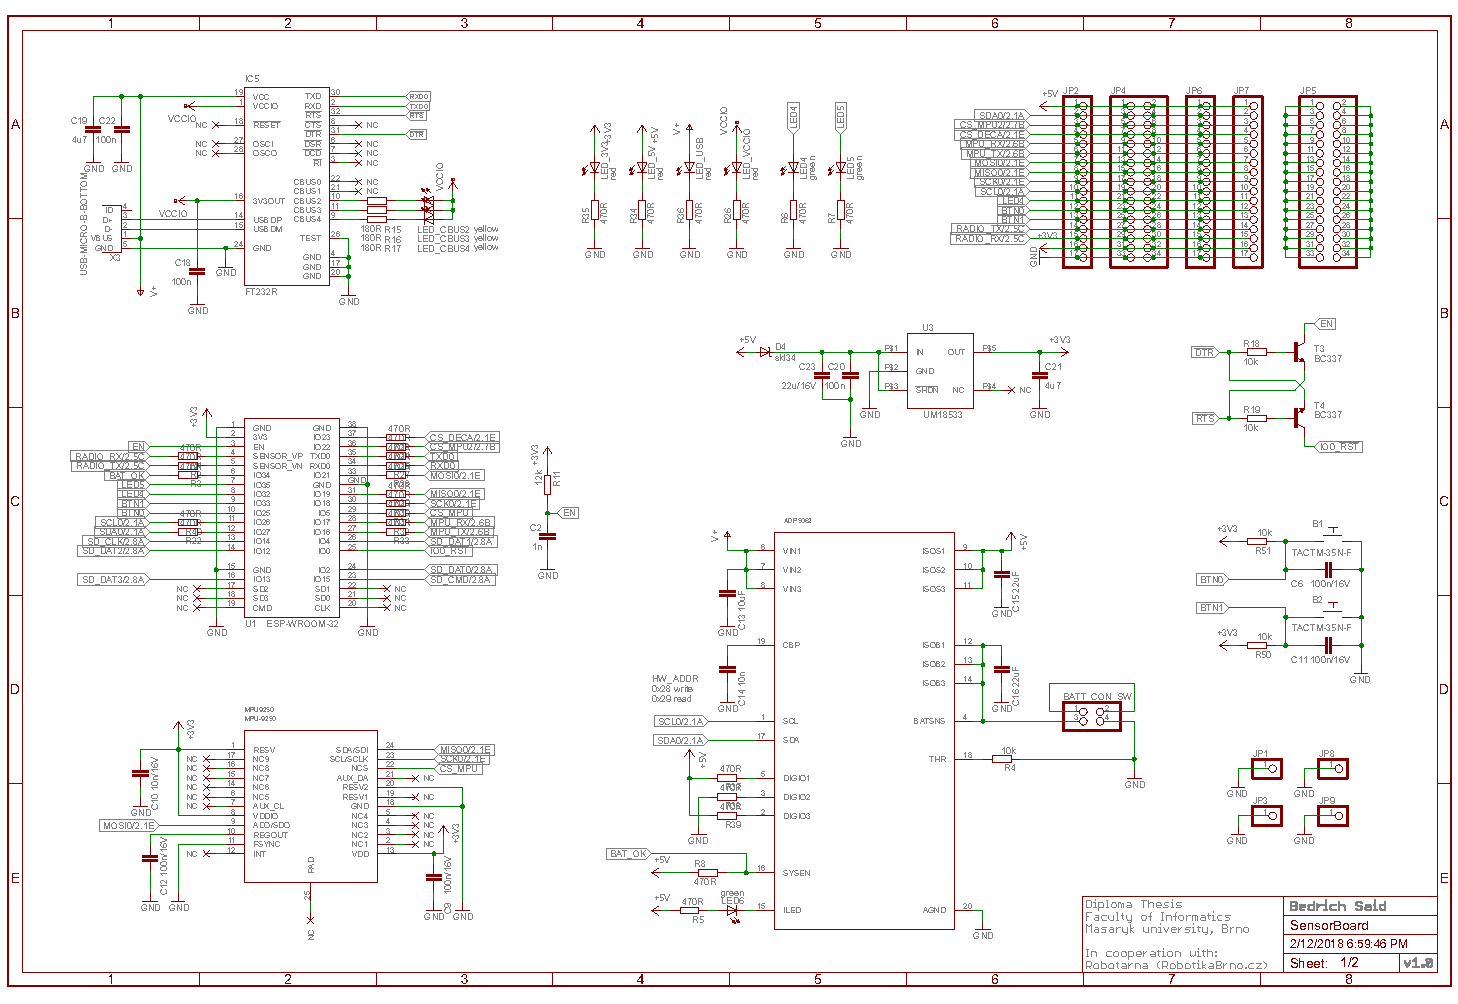
\includegraphics[angle=90, width=14cm]{img/sch1.pdf}
	\label{sch1}
	\caption{Schematics of the Sensor Board sheet 1}
\end{figure}

\begin{figure}
	\centering
	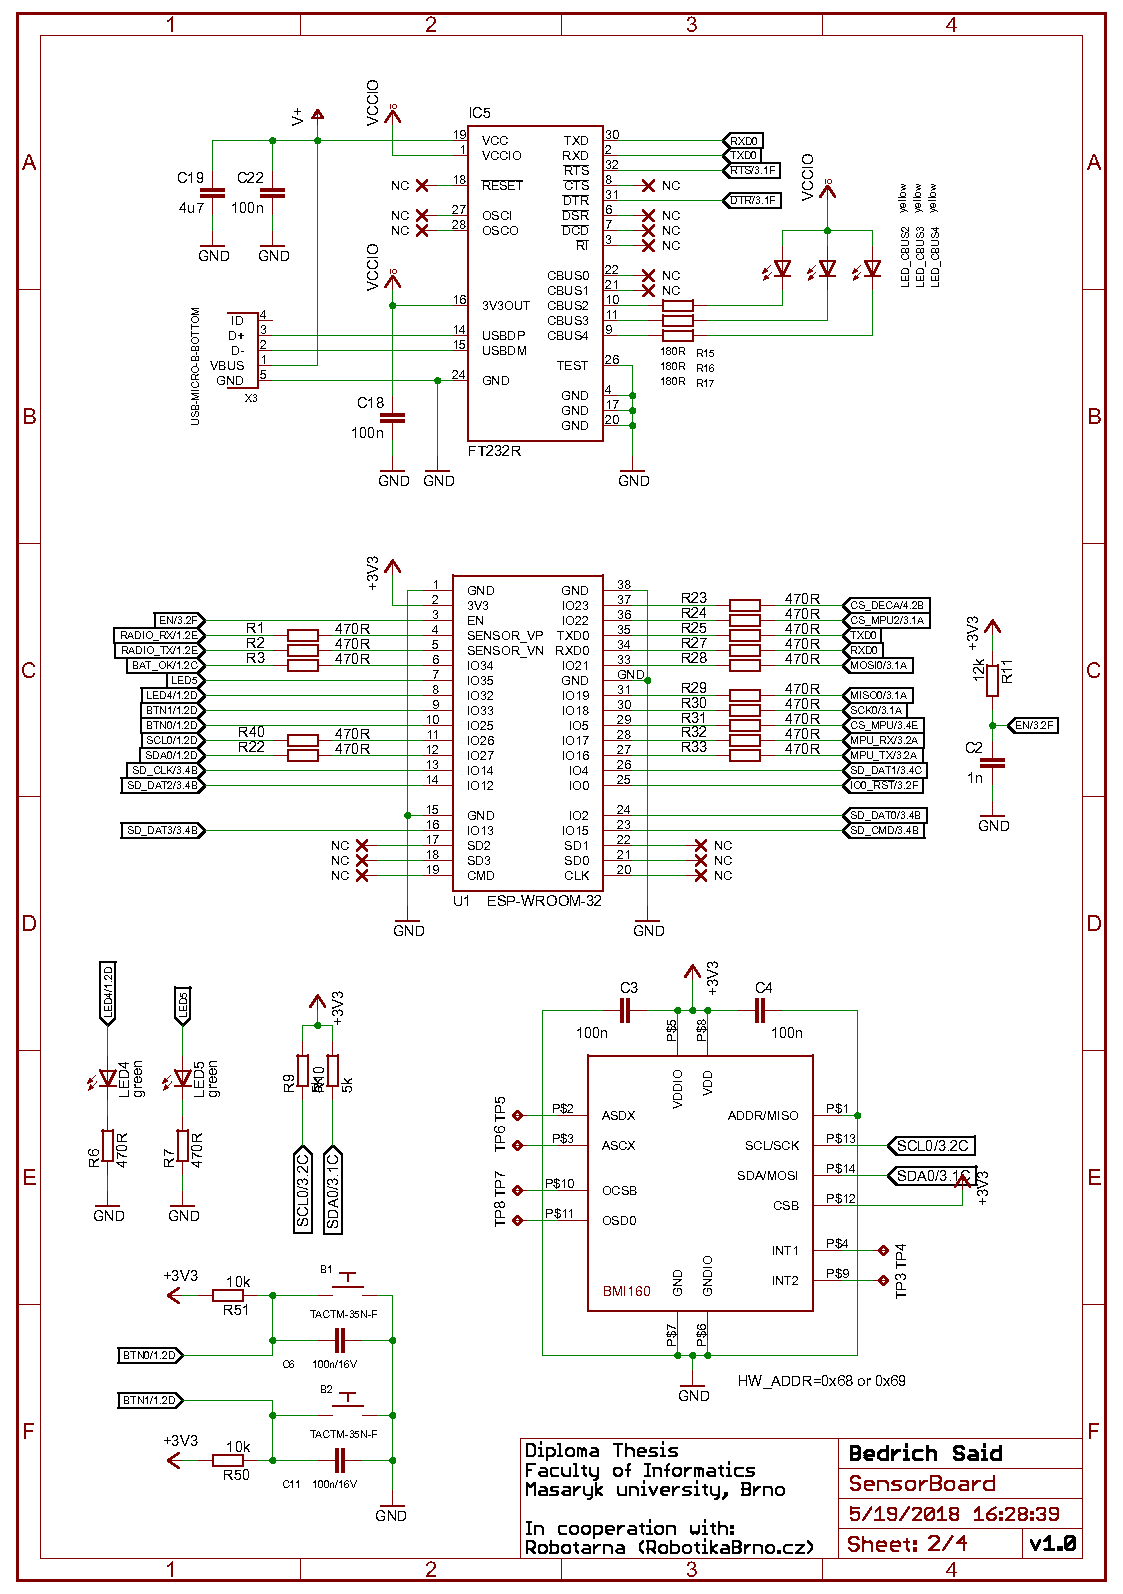
\includegraphics[angle=90, width=14cm]{img/sch2.pdf}
	\label{sch2}
	\caption{Schematics of the Sensor Board sheet 2}
\end{figure}

\begin{figure}
	\centering
	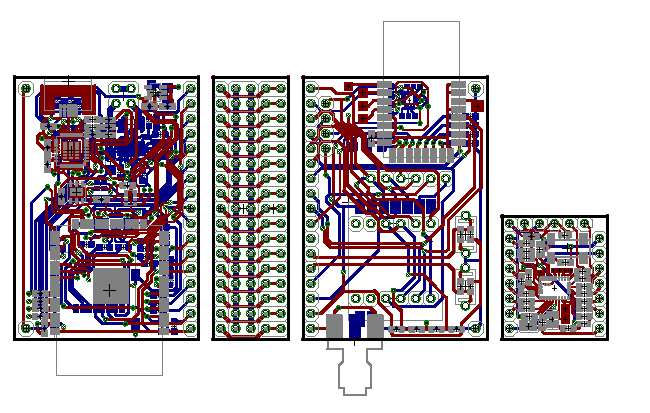
\includegraphics[scale=1]{img/brd.pdf}
	\vspace{-0.5cm}
	\begin{center}
		Top and Bottom layer
	\end{center}
	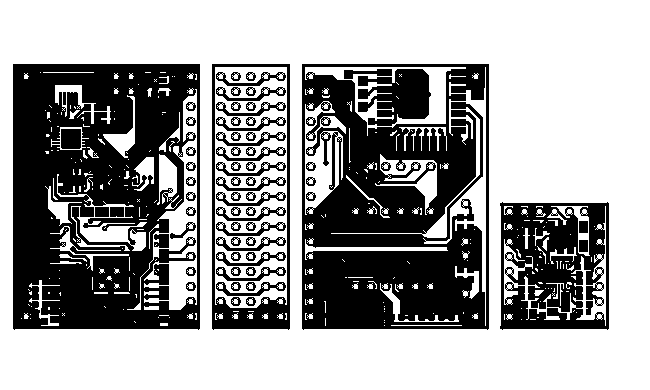
\includegraphics[scale=1]{img/brdTop.pdf}
	\vspace{-0.5cm}
	\begin{center}
		Only Top layer
	\end{center}
	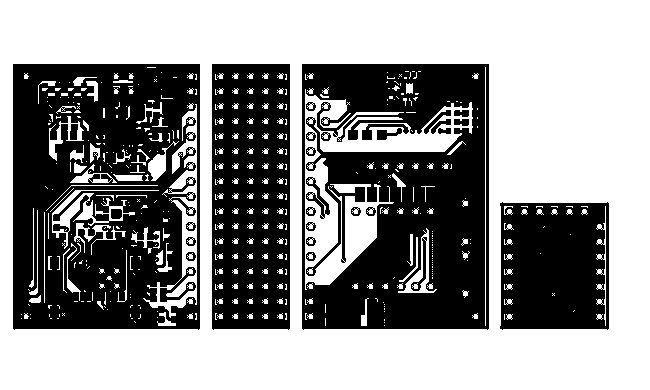
\includegraphics[scale=1]{img/brdBottom.pdf}
	\vspace{-0.5cm}
	\begin{center}
		Only Bottom layer
	\end{center}
	\label{brd1}
	\caption{Sensor Board layout in scale 1:1}
\end{figure}

\begin{figure}
	\centering
	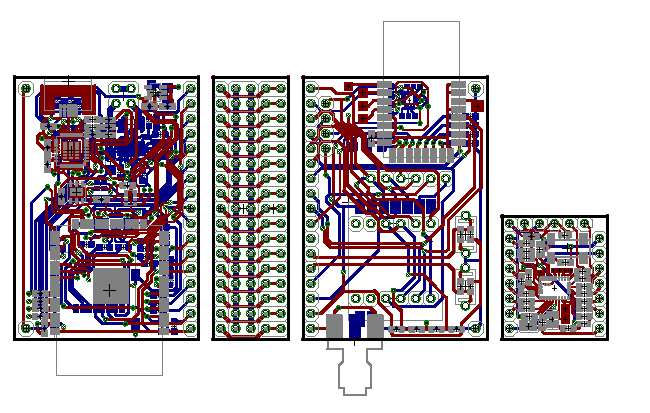
\includegraphics[angle=90, scale=2]{img/brd.pdf}
	\label{brd2}
	\caption{Sensor Board layout in detail scale 2:1}
\end{figure}

\subsection{Mechanical layout and connectors}
The mechanical layout is shown in figure \ref{fig:HWdimensions}.

\begin{figure}
	\centering
	\label{fig:HWdimensions}
	\caption{Sensor Board dimensions}
	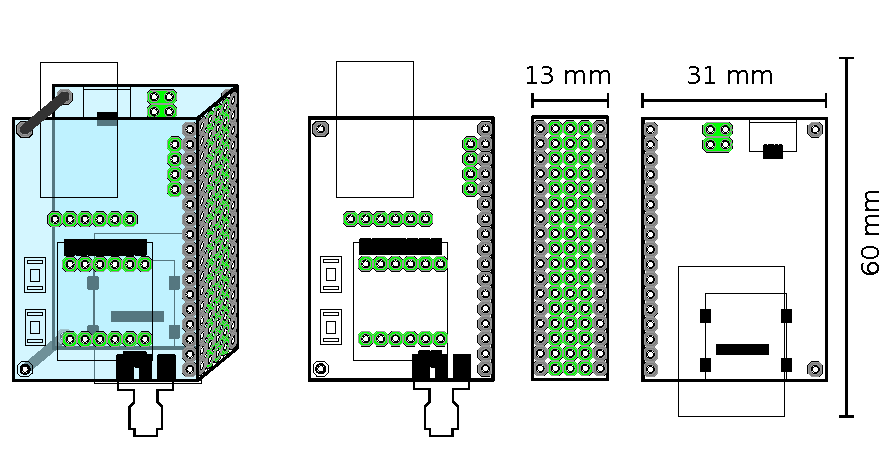
\includegraphics[scale=1]{img/HWdimensions.pdf}
\end{figure}

\section{Manufacturing}
\label{HWmanufacturing}

The manufacturing process of the prototype consists of these steps:
\begin{enumerate}
	\item Collecting source data -- schematics and board layout (in this paper in Eagle)
	\item Manufacturing of the Printed Circuit Board (\ac{PCB})
	\begin{enumerate}
		\item Panelization of the board layout
		\item Adding calibration markers
		\item Export gerber files
		\item Send exported files to manufacturing company
	\end{enumerate}
	\item Machine surface mount technology (\ac{SMT})
	\begin{enumerate}
		\item Export data for the template for applying solder paste
		\item Export partlist -- the list of all devices with their coordinates
		\item Export bill of materials (\ac{BOM})
		\item Manufacturing of the template for applying solder paste
		\item Order all devices according to \ac{BOM}
		\item Sending template for applying solder paste, packages with devices and part list to the manufacturer
	\end{enumerate}
	\item Finalization of the prototype
	\begin{enumerate}
		\item Hand soldering of some remaining devices like connectors or wires
		\item Completing the final prototype from possible parts and packaging
		\item Applying power and first testing
	\end{enumerate}
\end{enumerate}

\subsection{Collecting source data}
The source data may be in various formats according to the used tools. I used CadSoft \ac{EAGLE} \cite{EAGLE} during the development, but many other tools are available on the market. It depends on the manufacturer company if they accept the source data in our format. They usually accept the source data, but they usually apply an exporting fee. All \ac{PCB} editors should be able to export the manufacturing data in standardized formats. (Sometimes it's very hard or impossible to edit the exported data.)

\subsection{Manufacturing of the Printed Circuit Board}
When we have more than one board we should assemble all boards onto one or more panels. If we plan to solder the devices using the \ac{SMT}, we should add a calibration marks on the final panel. I have followed the instructions from SMTplus company \cite{SMTplusManual}.

First, I have panelized the separated boards and I have added the calibration marks according to the rules of SMTPlus company \cite{SMTPlusDesignRules}. Finally, I have exported the Gerber files using a CAM job \cite{GatemaCAMjob} in \ac{EAGLE}. I have followed the design rules for class 3 by Gatema a.s. company \cite{GatemaDesignRules}.

\subsection{Machine surface mount technology}
We need the \ac{PCB}, template for soldering paste and all devices in this step. Some \ac{PCB} manufacturers offer to create the template as well, so this is the way I used. The thickness of the template indicates the volume of the paste on each pad. For the small \ac{SMD} parts I used \SI{100}{\micro\meter}, but I recommend to discuss the parameters with the manufacturer.

The \ac{BOM} and part list export depends on the used design tools. When we connect used devices in the sources directly with their part numbers on selected shops, we can simply export the part list and then import it on the seller's website. I recommend buying some spare devices to minimize the risk of their damage.

\begin{figure}
	\centering
	\label{smtPasteTemplate}
	\caption{Template for soldering paste in scale 1:2}
	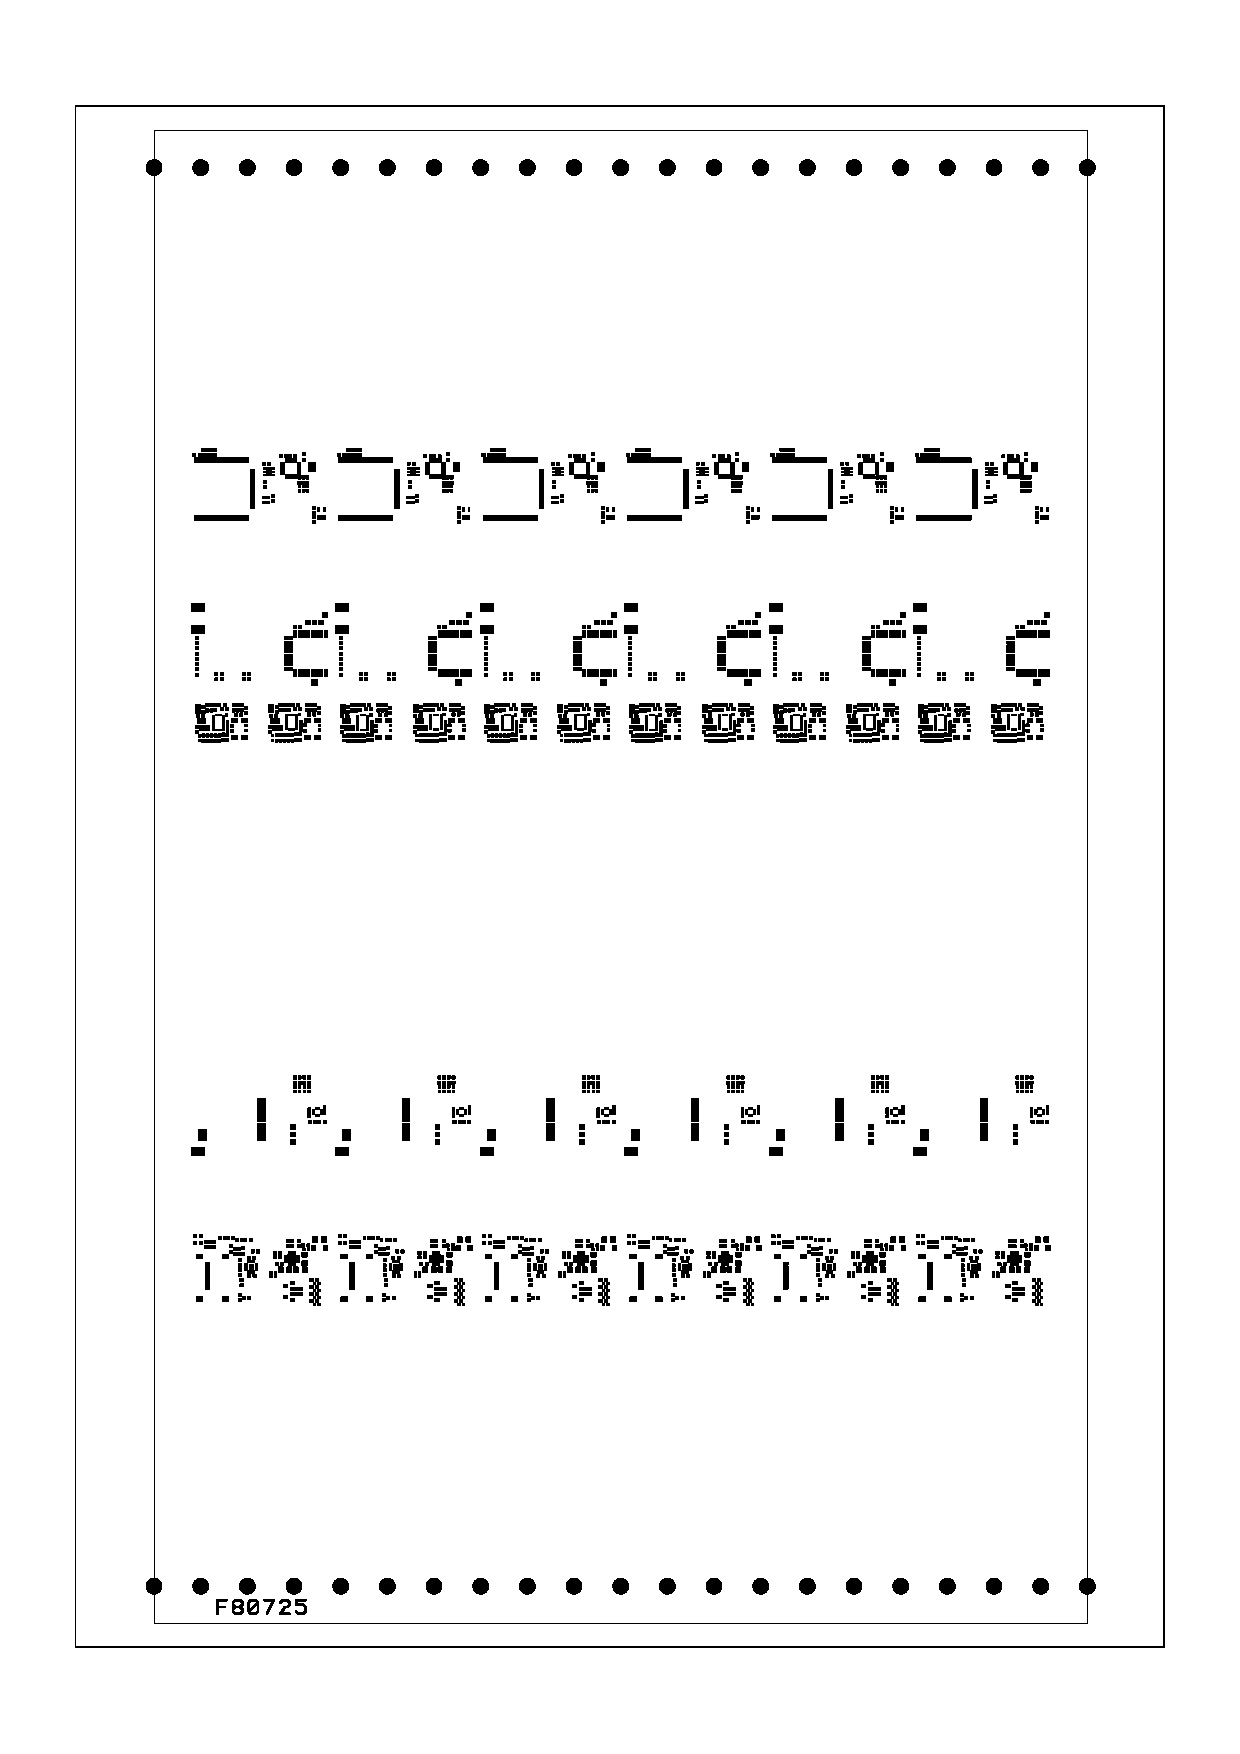
\includegraphics[angle=90, scale=0.5]{img/smtPasteTemplate.pdf}
\end{figure}

\subsection{Finalization of the prototype}
We can discuss the finalization works with the manufacturer, but when we create a prototype, I would like to recommend to do this job by yourself. It allows us to perform some tests before packaging and we don't have to spend time and money with a preparation of the documentation about how to assemble and package our prototype. Otherwise, the different software developers and testers can receive the different parts of the prototype for their next work.

\section{Testing}
\label{HWtesting}
The testing process has been split into two parts: the laboratory testing during the software development and the outdoor testing. I have found some errors in the version 1.0 during the laboratory testing. These errors are described in Errata list in section \ref{errata}. I did other tests against the specification of used devices. The results show us what devices should be used in the next version of the hardware and what devices are redundant. The results are shown in the section \ref{deviceTesting}. The outdoor tests didn't find any significant errors, but there were found several recommendations for the future versions of the SensorBoard. These recommendations are mentioned in section \ref{recommendationsNextVerison}.

\subsection{Errata}
\label{errata}
The tables \ref{tab:errata} and \ref{tab:errata2} show all errors I have found during software development and laboratory testing of the Sensor Board prototype.

\begin{table}
	\centering
	\caption{Errata of the SensorBoard}
	\label{tab:errata}
	\begin{tcolorbox}[tab2,tabularx={X|p{12cm}},title=Severity legend]
		\greenLow & No significant affects \\
		\greenSpare & Only spare devices may not work \\
		\yellowMedium & Some part of the prototype may not work \\
		\redHigh & The prototype has to be remade \\
	\end{tcolorbox}
	\vspace{1cm}
	\begin{tcolorbox}[tab2,tabularx={|c|p{7.5cm}|X|c|},title=Errata 1 of 2]
		Number & Description & Error created during & Severity \\ \hline
		1      &
		\parbox{7.5 cm}{\quad\\Bridge between boards under micro USB connector\\ \\ What happens:\\ The micro USB connector may be placed with lower accuracy\\}
		& panelization         & \greenLow      \\ \hline
		
		2      &
		\parbox{7.5 cm}{\quad\\Swapped MISO and MOSI on pins IO19 and IO21 on the ESP-WROOM-32 chip according to ESP32 Arduino standard\\ \\ What happens:\\ The SPI interface is not working in Arduino compatible mode without modification of the Arduino SPI library\\}
		& schematics design    & \yellowMedium   \\ \hline
		
		3      &
		\parbox{7.5 cm}{\quad\\LED5 connected to IO35 on ESP-WROOM-32 is not working\\ \\ What happens:\\ The pins IO34 -- IO39 are input only, so they cannot drive a LED\\}
		& schematics design    & \greenSpare    \\ \hline
		
		4      &
		\parbox{7.5 cm}{\quad\\Missing pull-up resistors on SD card\\ \\ What happens:\\ The SDIO interface needs external pull-up resistors to work properly. I have added these resistors later by hand.\\}
		& schematics design    & \yellowMedium   \\ \hline
	\end{tcolorbox}
\end{table}

\begin{table}
	\centering
	\caption{Errata of the SensorBoard}
	\label{tab:errata2}
	\begin{tcolorbox}[tab2,tabularx={|c|p{7.5cm}|X|c|},title=Errata 2 of 2]
		Number & Description & Error created during & Severity \\ \hline
		
		5      &
		\parbox{7.5 cm}{\quad\\The temperature measurement is placed very close to the main processor\\ \\ What happens:\\ The processor heating affects the measured temperature\\}
		& board layout         & \greenSpare    \\ \hline
		
		6      &
		\parbox{7.5 cm}{\quad\\Low capacity capacitor placed on power supply\\ \\ What happens:\\ When we use WiFi some brownouts can be detected. I have added a bigger capacitor later by hand.\\}
		& schematics design    & \yellowMedium   \\ \hline
		
		7      &
		\parbox{7.5 cm}{\quad\\The light sensor is placed on inner side of the board\\ \\ What happens:\\ The measured values are affected by shadow of the board.\\}
		& board layout         & \greenSpare    \\ \hline
		8      &
		\parbox{7.5 cm}{\quad\\Missing safety resistors on pins with buttons. These pins are directly connected to processor.\\ \\ What happens:\\ When the pins are defined in software to be used in different way, incorrect connection can burn the processor.\\}
		& schematics design        & \yellowMedium   \\ \hline
	\end{tcolorbox}
\end{table}

\subsection{Device testing}
\label{deviceTesting}
The device testing helped me to select the parts recommended for the future versions of the SensorBoard. It also helped me to mark all spare parts in the prototype. The table \ref{tab:deviceSelection} shows the results.

\begin{table}
	\centering
	\caption{Parts of the SensorBoard recommended for the future versions}
	\label{tab:deviceSelection}
	\begin{tcolorbox}[tab2,tabularx={X|p{12cm}},title=Decision legend]
		\greenCell{Selected} & Recommended for use in future versions \\ \hline
		\yellowCell{Possible} & Not necessary, but has use-cases, may be replaced with another part \\ \hline
		\redCell{Removed} & Not recommended or will be spare \\ \hline
	\end{tcolorbox}
	\vspace{1cm}
	\begin{tcolorbox}[tab2,tabularx={|X|p{7cm}|c|c|},title=Parts of the SensorBoard recommended for the future versions]
		Part ID & Description & Datasheet & Selected \\\hline\hline
		TACTM-35N-F & Button & \cite{TACTM} & \greenCell{Selected} \\
		ADP5062 & Power management and battery charger & \cite{analogdevices:ADP5062} & \greenCell{Selected} \\
		SI7006 & Humidity and temperature sensor & \cite{siliconlabs:SI7006} & \greenCell{Selected} \\
		DWM1000 & \ac{TDOA} location sensor (with antenna) & \cite{decawave:DWM1000} & \greenCell{Selected} \\
		BMP280 & Barometer & \cite{bosch:BMP280} & \greenCell{Selected} \\
		FT232R & UART to USB converter & \cite{ftdichip:FT232R} & \greenCell{Selected} \\
		MPU-9250 & Accelerometer, dynamic gyroscope, magnetometer & \cite{invensense:MPU9250} & \redCell{Removed} \\
		BMI160 & Accelerometer, dynamic gyroscope & \cite{bosch:BMI160} & \redCell{Removed} \\
		BMF055 & Accelerometer, dynamic gyroscope, magnetometer, ARM microcontroller & \cite{bosch:BMF055} & \greenCell{Selected} \\
		GY953 & Backup accelerometer, dynamic gyroscope and megnetometer with embedded pitch, roll and yaw angle estimation (sensor fusion) & \cite{GY953} & \redCell{Removed} \\
		HM-TRP & Long range \SI{433}{MHz} radio & \cite{HM-TRP} & \yellowCell{Possible} \\
		MOLEX-47219-2001 & Micro SD card holder & \cite{MOLEX-SD1} & \greenCell{Selected} \\
		LTR-329ALS & Digital ambient light sensor & \cite{LTR-329ALS} & \greenCell{Selected} \\
		ESP-WROOM-32 & Dual core controller with WiFi and Bluetooth & \cite{espressif:ESP-WROOM-32} & \greenCell{Selected} \\
		UM18533 & \parbox{7 cm}{Linear stabilizer \SI{3.3}{V} \\\\ Note: Insufficient current} & \cite{UM18533} & \redCell{Removed} \\
		LF33 & Linear stabilizer \SI{3.3}{V} & \cite{LF33} & \greenCell{Selected} \\
		USB-MICRO & Micro USB connector & \cite{USB-MICRO} & \greenCell{Selected} \\
		Pin header 2.54 mm & Servo connector & \cite{PINHEAD} & \yellowCell{Possible} \\
	\end{tcolorbox}
\end{table}

\subsection{Recommendations for the next version}
\label{recommendationsNextVerison}
Recommendations for the future versions of the Sensor Board based on the outdoor testing:
\begin{itemize}
	\item[--] Replace software LEDs by one or more RGB LEDs. For example WS2812 RGB LED \cite{AdafruitLED}.
	\item[--] Move the sensor fusion and computations to Atmel SAM D21 \cite{AtmelSAM} processor inside the BMF055 \cite{BMF055} chip. Keep the ESP32 \cite{ESP32} processor only for communication and user computations.
	\item[--] Decrease board dimensions using 4 layer \ac{PCB}. The increased cost for 4 layer board may be saved on a smaller surface.
	\item[--] Sometimes it is better to have all \ac{SMD} parts on one side of the board. The manufacturing is cheaper and the space on the second side can be used for example for battery mounting or for connectors.
	\item[--] Split the board area to an area for sensors, an area for power electronics and an area for computing. The power distribution is easier in this situation and the sensors are less influenced by other electronics.
	\item[--] Use another driver with more capabilities for USB connection. The USB on board actually supports only UART communication on the virtual COM port. The File Transfer protocol for the SD card should be supported, too. (If it is needed we can add full USB host support or USB-C compatibility.)
	\item[--] Add specialized pads for an oscilloscope. The pads are connected to the signal and to the ground, so the oscilloscope measurements are more accurate.
	\item[--] The main processor should be able to switch on/off the power of other parts (sensors). The sensors support sleep modes, but we cannot completely switch them off to save more energy from the battery.
	\item[--] If we recognize that the ESP-WROOM-32 controller is not powerful enough, we can use a fully compatible alternative with larger memory ALB32-WROVER \cite{ALB32-WROVER}. It should be possible to compile a terminal based Linux distribution for this controller.
\end{itemize}

\subsection{Analysis of additional costs}
\label{HWadditionalCosts}
By the analysis of additional costs, I mean the counting the prices of all parts that were finally spare or weren't used. The table \ref{tab:additionalCost} counts all parts of the SensorBoard and their prices.

The column "Used" tells us if the item was used for any use case or if it was spare at all times. If any item is still unused it doesn't mean that it cannot be used in some future use case. The column "Is necessary" points the basic items, the SensorBoard can't work or can't be built without them.

It means that the green cost "Total used and necessary" is the lowest cost of the prototype without any additional functionality. The yellow cost "Total used and unnecessary" is the cost of all items that had significant value during development, but weren't mandatory for the main task. These items also made the development process easier and faster, so I don't count this cost as additional. The last red cost "Total unused" covers all items that weren't used. These items were a part of the design because they lowered some risks in functionality. For example, if I wasn't sure that an accelerometer will work properly, I added another spare accelerometer, which covered this risk. I could get a working prototype in the first iteration using this strategy. I finally count the red cost as a cost of decreased risks and as a cost of higher versatility.

We have to take into account that all the mentioned costs are costs of the prototype. The same items would have significantly lower costs during the production of more devices.

\begin{table}
	\centering
	\caption{Additional cost calculation}
	\label{tab:additionalCost}
	\begin{tcolorbox}[tab2,tabularx={|X|l|c|c|},title=Additional cost calculation]
		Part ID & Price & Used & Is necessary \\\hline\hline
		\ac{PCB} & \$ 23 & \greenYes & \greenYes \\
		\ac{SMT} job & \$ 65 & \greenYes & \greenYes \\ \hline
		TACTM-35N-F & \$ 0.4 & \greenYes & \yellowCell{No} \\
		ADP5062 & \$ 3.8 & \greenYes & \greenYes \\
		SI7006 & \$ 2 & \redNo & \redNo \\
		DWM1000 & \$ 22 & \greenYes & \yellowCell{No} \\
		BMP280 & \$ 4 & \greenYes & \yellowCell{No} \\
		FT232R & \$ 5 & \greenYes & \greenYes \\
		MPU-9250 & \$ 10 & \greenYes & \yellowCell{No} \\
		BMI160 & \$ 4.3 & \redNo & \redNo \\
		BMF055 & \$ 11 & \greenYes & \greenYes \\
		GY953 & \$ 11 & \redNo & \redNo \\
		HM-TRP & \$ 13 & \greenYes & \yellowCell{No}\\
		MOLEX-47219-2001 & \$ 1.2 & \greenYes & \greenYes \\
		LTR-329ALS & \$ 0.7 & \redNo & \redNo \\
		ESP-WROOM-32 & \$ 12 & \greenYes & \greenYes \\ \hline \hline
		\greenCell{\textbf{Total used and necessary}} & \greenCell{\textbf{\$ 121}} & \greenYes & \greenYes \\
		\yellowCell{\textbf{Total used and unnecessary}} & \yellowCell{\textbf{\$ 49.4}} & \yellowCell{Yes} & \yellowCell{No} \\
		\redCell{\textbf{Total unused}} & \redCell{\textbf{\$ 18}} & \redNo & \redNo \\
	\end{tcolorbox}
\end{table}

\chapter{Software}
The Sensor Board hardware has two programmable CPUs and several configurable chips. The main ESP32 CPU (two low-power Xtensa 32-bit LX6 microprocessors) \cite{espressif:ESP-WROOM-32} is programmable via USB or Bluetooth or \ac{JTAG}. The \ac{JTAG} connector is not present on the Sensor Board. The second microcontroller is a part of BMF055 \cite{bosch:BMF055} multifunctional chip. It is Atmel SAMD20 \cite{atmel:SAMD20} with ARM Cortex-M0+ CPU programmable via \ac{SWD} interface \cite{SWDinterface}.

\paragraph{Microcontrollers:}
\begin{enumerate}
	\item Espressif ESP-WROOM-32 \cite{espressif:ESP-WROOM-32}:
	\begin{itemize}
		\item dual core, 240 MHz, 448 kB ROM, 520 kB SRAM, 4 MB SPI flash memory
		\item Designated for main program handling all communication and interaction with user or other devices.
	\end{itemize}
	\item Atmel SAMD20 \cite{atmel:samd20}:
	\begin{itemize}
		\item ARM Cortex-M0+ CPU, 48 MHz, 32 kB SRAM, 256 kB flash memory
		\item Designated for processing inertial data (for example computing sensor fusion), it can be used for example as an emulator of other sensors or as a simple flight controller.
	\end{itemize}
\end{enumerate}

\begin{figure}
	\centering
	\label{fig:SWmodules}
	\caption{Schema of the available modules inside the SensorBoard hardware}
	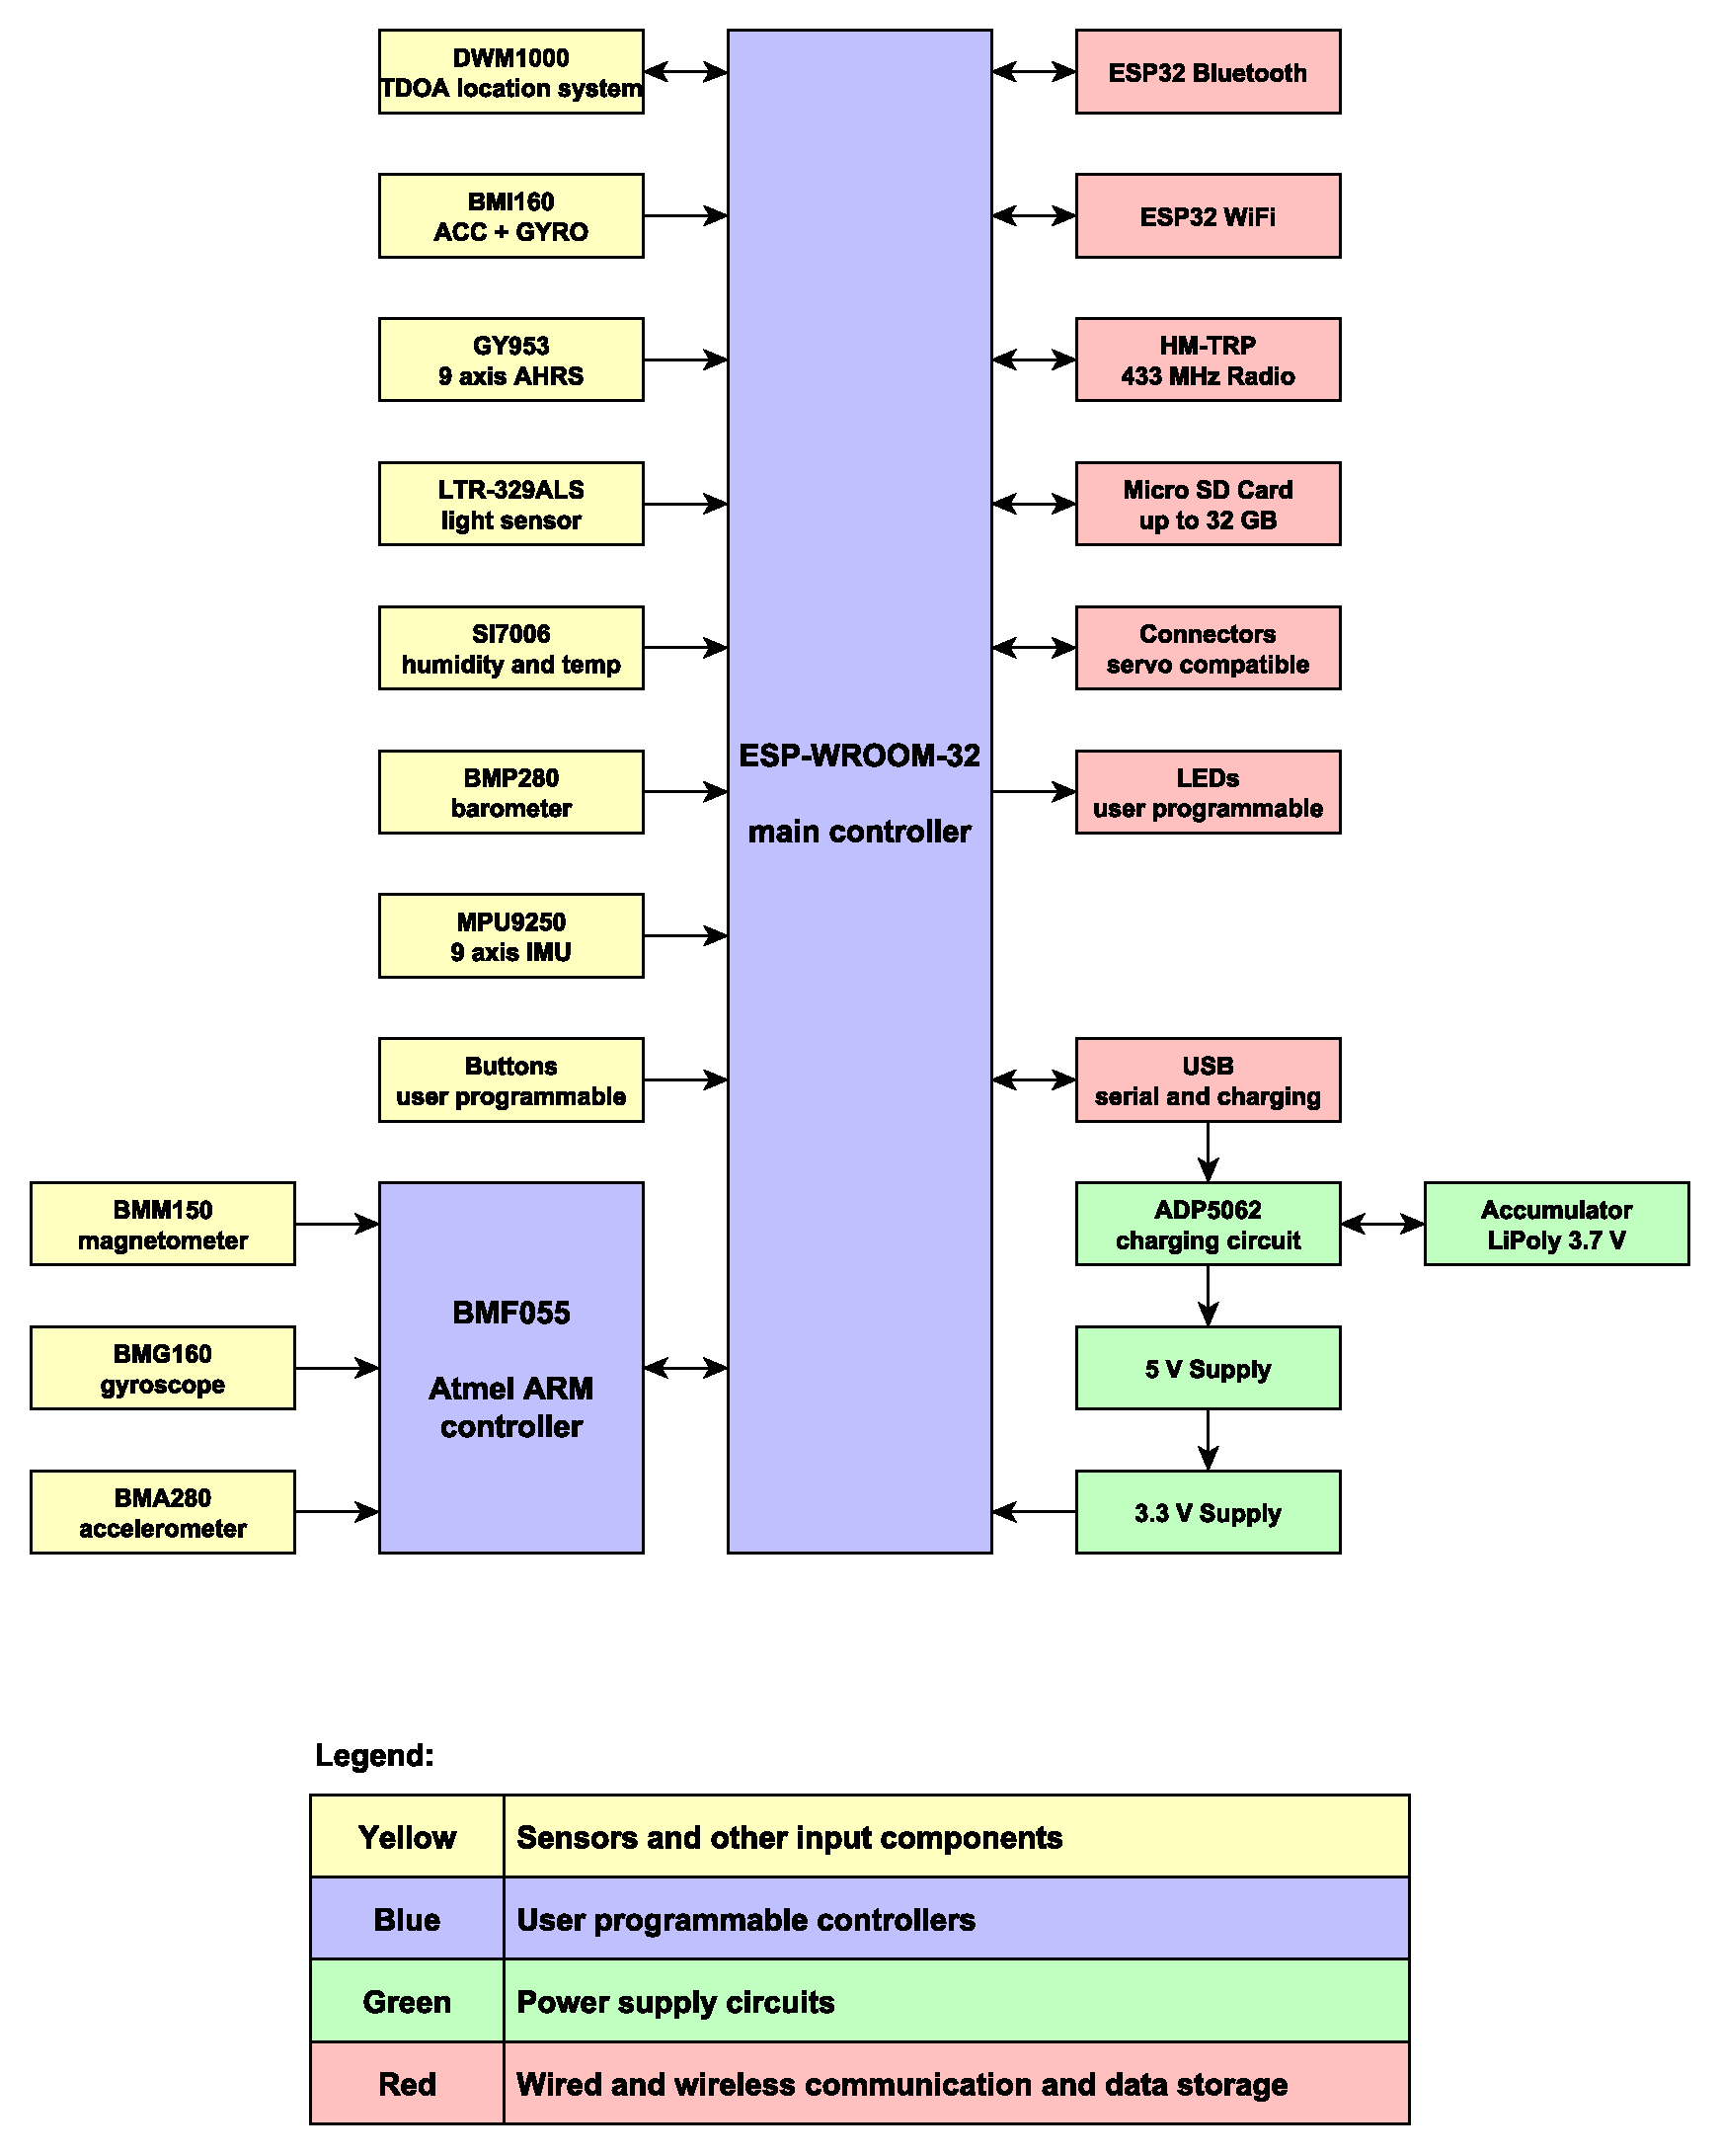
\includegraphics[width=\linewidth]{img/SensorBoardSchema.pdf}
\end{figure}

\section{Programming the Board}
Each processor on the SensorBoard has to be programmed separately via its interface. Only ESP32 \cite{espressif:ESP-WROOM-32} (main processor) can be programmed over the air via Bluetooth. This feature is disabled by default. The pinout and other information about the SensorBoard and BMF055 board are described in appendix \ref{hardwareDocumentation}.

\subsection{Programming ESP32}
There are several ways how to program and use the ESP32 \cite{espressif:ESP-WROOM-32} controller. The official framework is Espressif \ac{IoT} Development Framework (\ac{ESP-IDF}) \cite{espressif:ESP-IDF} and supports all the chip functionality. The \ac{ESP-IDF} framework is \ac{POSIX} compatible.

The chip can be programmed using Arduino compatible framework \cite{espressif:ArduinoCore} which creates an easy way for prototyping and learning, but does not offer all the functionality of the chip. The Arduino framework uses the \ac{ESP-IDF} framework, so we can create "hybrid" programs that use both frameworks.

The last mentioned programming method is scripting in Python. We can upload the MicroPython \cite{MicroPython} firmware directly to the ESP32 controller. The Python libraries, scripts and other files are stored on the SD card. The MicroPython firmware supports most of the hardware functionality, but there are still some restrictions.

There are some other ways how to create a program for this hardware, but many of them use one of the mentioned frameworks. For example, we can create a program in Simulink and then export the code to the ESP32 controller. \cite{ArduinoSimulink}

\subsubsection{\ac{ESP-IDF} Framework}
The \ac{ESP-IDF} framework is almost \ac{POSIX} compatible. \cite{ESP32posix} It supports many \ac{POSIX} compatible functions, but it still doesn't support all of them. It means that we can compile many \ac{POSIX} compatible programs for ESP32, but not all of them.

We can follow the official ESP32 programming guide \cite{ESP32programmingGuide} to set up the environment and program the board. The user can do everything from the terminal (command line). The figure \ref{ESP32menuconfig} shows a configuration tool used for setup the program before the first compilation and upload to the ESP32 microcontroller.

\begin{figure}
	\centering
	\label{ESP32menuconfig}
	\caption{Configuration of the \ac{ESP-IDF} program in terminal before the first compilation}
	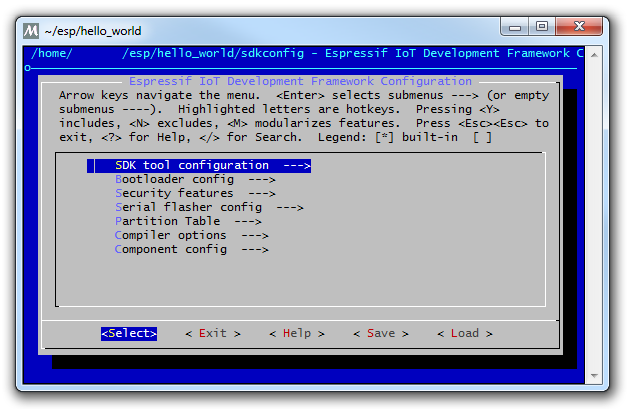
\includegraphics[width=\linewidth]{img/ESP32menuconfig.png}
\end{figure}

If we prefer some GUI for development of our software we have several options. I will mention two of them:
\begin{enumerate}
	\item \textbf{Eclipse IDE} can be setup using the guide in \ac{ESP-IDF} Programming Guide \cite{ESP32eclipse}. In my opinion, the compilation of our programs is very slow when we use this option. The figure \ref{ESP32eclipse} shows the SensorBoard project opened in Eclipse IDE.
	\item \textbf{PlatformIO IDE} is an open source ecosystem for \ac{IoT} development. \cite{PlatformIO} There is integrated \ac{ESP-IDF} and Arduino framework for ESP32 microcontrollers. This option was more familiar to me with much faster compilation process. I have used the PlatformIO ecosystem inside Atom \cite{AtomEditor} advanced text editor. The figure \ref{ESP32atom} shows the SensorBoard project opened in Atom editor with PlatformIO plugin.
\end{enumerate}

\begin{figure}
	\centering
	\label{ESP32eclipse}
	\caption{The SensorBoard project opened in Eclipse IDE}
	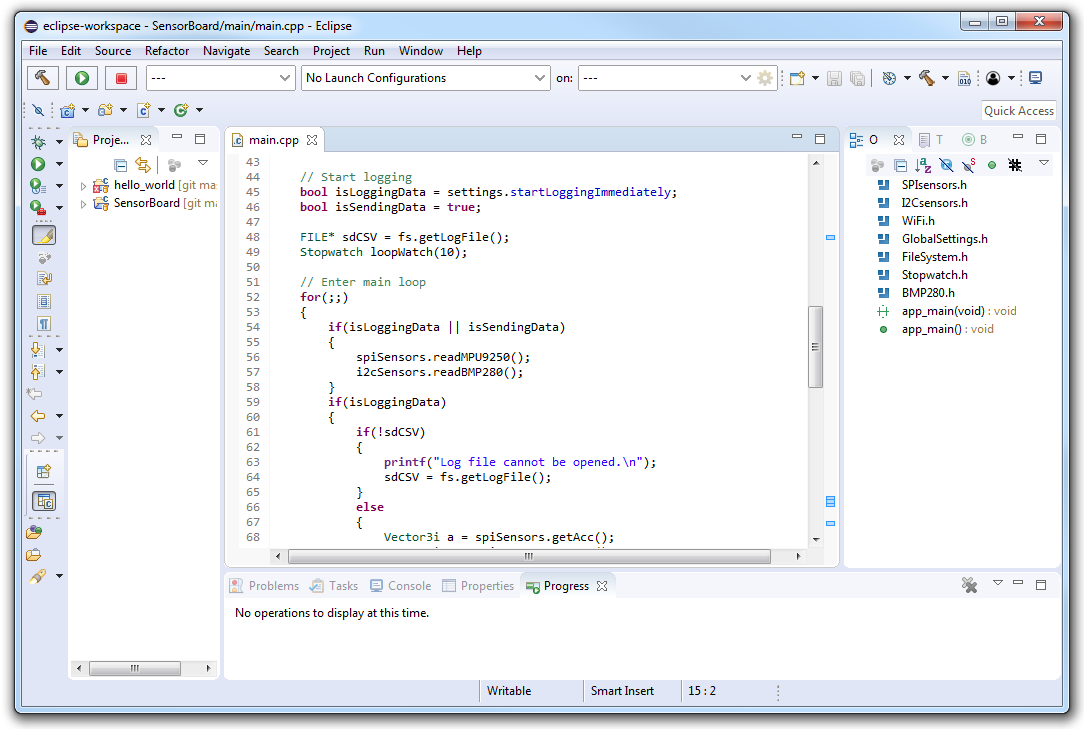
\includegraphics[width=\linewidth]{img/ESP32eclipse.png}
\end{figure}

\begin{figure}
	\centering
	\label{ESP32atom}
	\caption{The SensorBoard project opened in Atom text editor with PlatformIO plugin}
	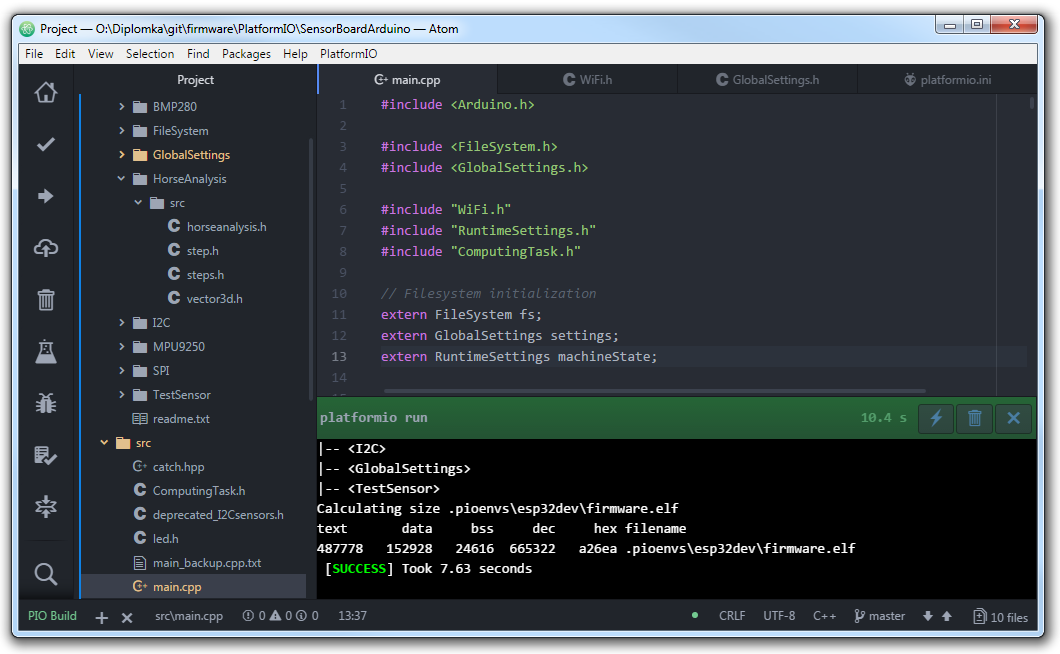
\includegraphics[width=\linewidth]{img/ESP32atom.png}
\end{figure}

\subsubsection{Arduino Compatibility}
The Arduino compatible framework for ESP32 \cite{espressif:ArduinoCore} is dependent on \ac{ESP-IDF} framework \cite{espressif:ESP-IDF}. It means that we can use both -- the \ac{ESP-IDF} functions and the Arduino functions -- in our programs. The Arduino framework is primarily targeted for beginners and for fast prototyping. I don't recommend to use this framework for advanced applications, because it doesn't cover the whole ESP32 functionality. We can develop our Arduino compatible programs in Arduino IDE, but we can use the PlatformIO ecosystem, too. It means that we can use the same environment like in the figure \ref{ESP32atom}. All libraries are downloaded and installed automatically inside the PlatformIO. We have to set only a \texttt{platformio.ini} file in the root directory of our project. We can add a line \texttt{framework = arduino} for Arduino compatible programs and a line \texttt{framework = espidf} for programs using the \ac{ESP-IDF} framework.

\subsubsection{MicroPython Compatibility}
The built MicroPython binary for ESP32 can be directly downloaded from MicroPython website. \cite{MicroPython} We can directly flash this binary to our ESP32 controller (to the SensorBoard) and then directly run our Python scripts. Of course, it is possible to download the MicroPython source code from the same website. The MicroPython allows to control the SensorBoard via Python serial terminal, so we can send a separate command via this serial terminal or run the whole Python scripts stored as files in the SD card. The SD card slot is a part of the SensorBoard. One of the Python scripts on the SD card can be configured to be executed automatically after powering on the SensorBoard. The running Python serial terminal on the SensorBoard is shown in figure \ref{ESP32PythonLorris}.

\begin{figure}
	\centering
	\label{ESP32PythonLorris}
	\caption{The running Python serial terminal on the SensorBoard}
	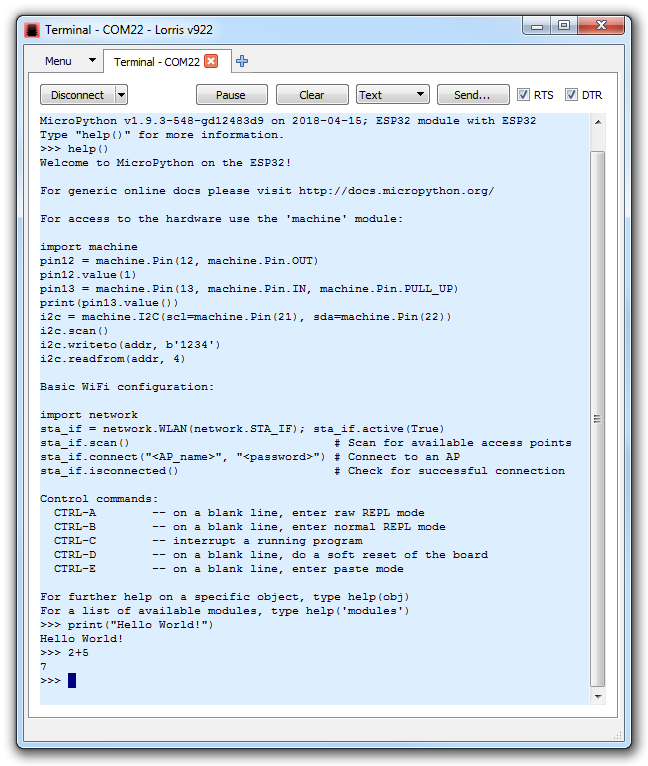
\includegraphics[width=\linewidth]{img/PythonESP.png}
\end{figure}

\subsection{Programming BMF055}
The BMF055 \cite{bosch:BMF055} is a custom programmable 9-axis motion sensor. It is a single chip triaxial accelerometer, dynamic gyroscope, magnetometer and ARM controller. The BMF055 chip is mounted on a separate board which can be optionally mounted to the SensorBoard or it can be used independently. The figure \ref{BMF055photo} shows the separate BMF055 board and the same board mounted to the SensorBoard.

\begin{figure}
	\centering
	\label{BMF055photo}
	\caption{The separate BMF055 board on the left and the same board mounted to the Sensor board on the right}
	\begin{minipage}[c]{.45\textwidth}
		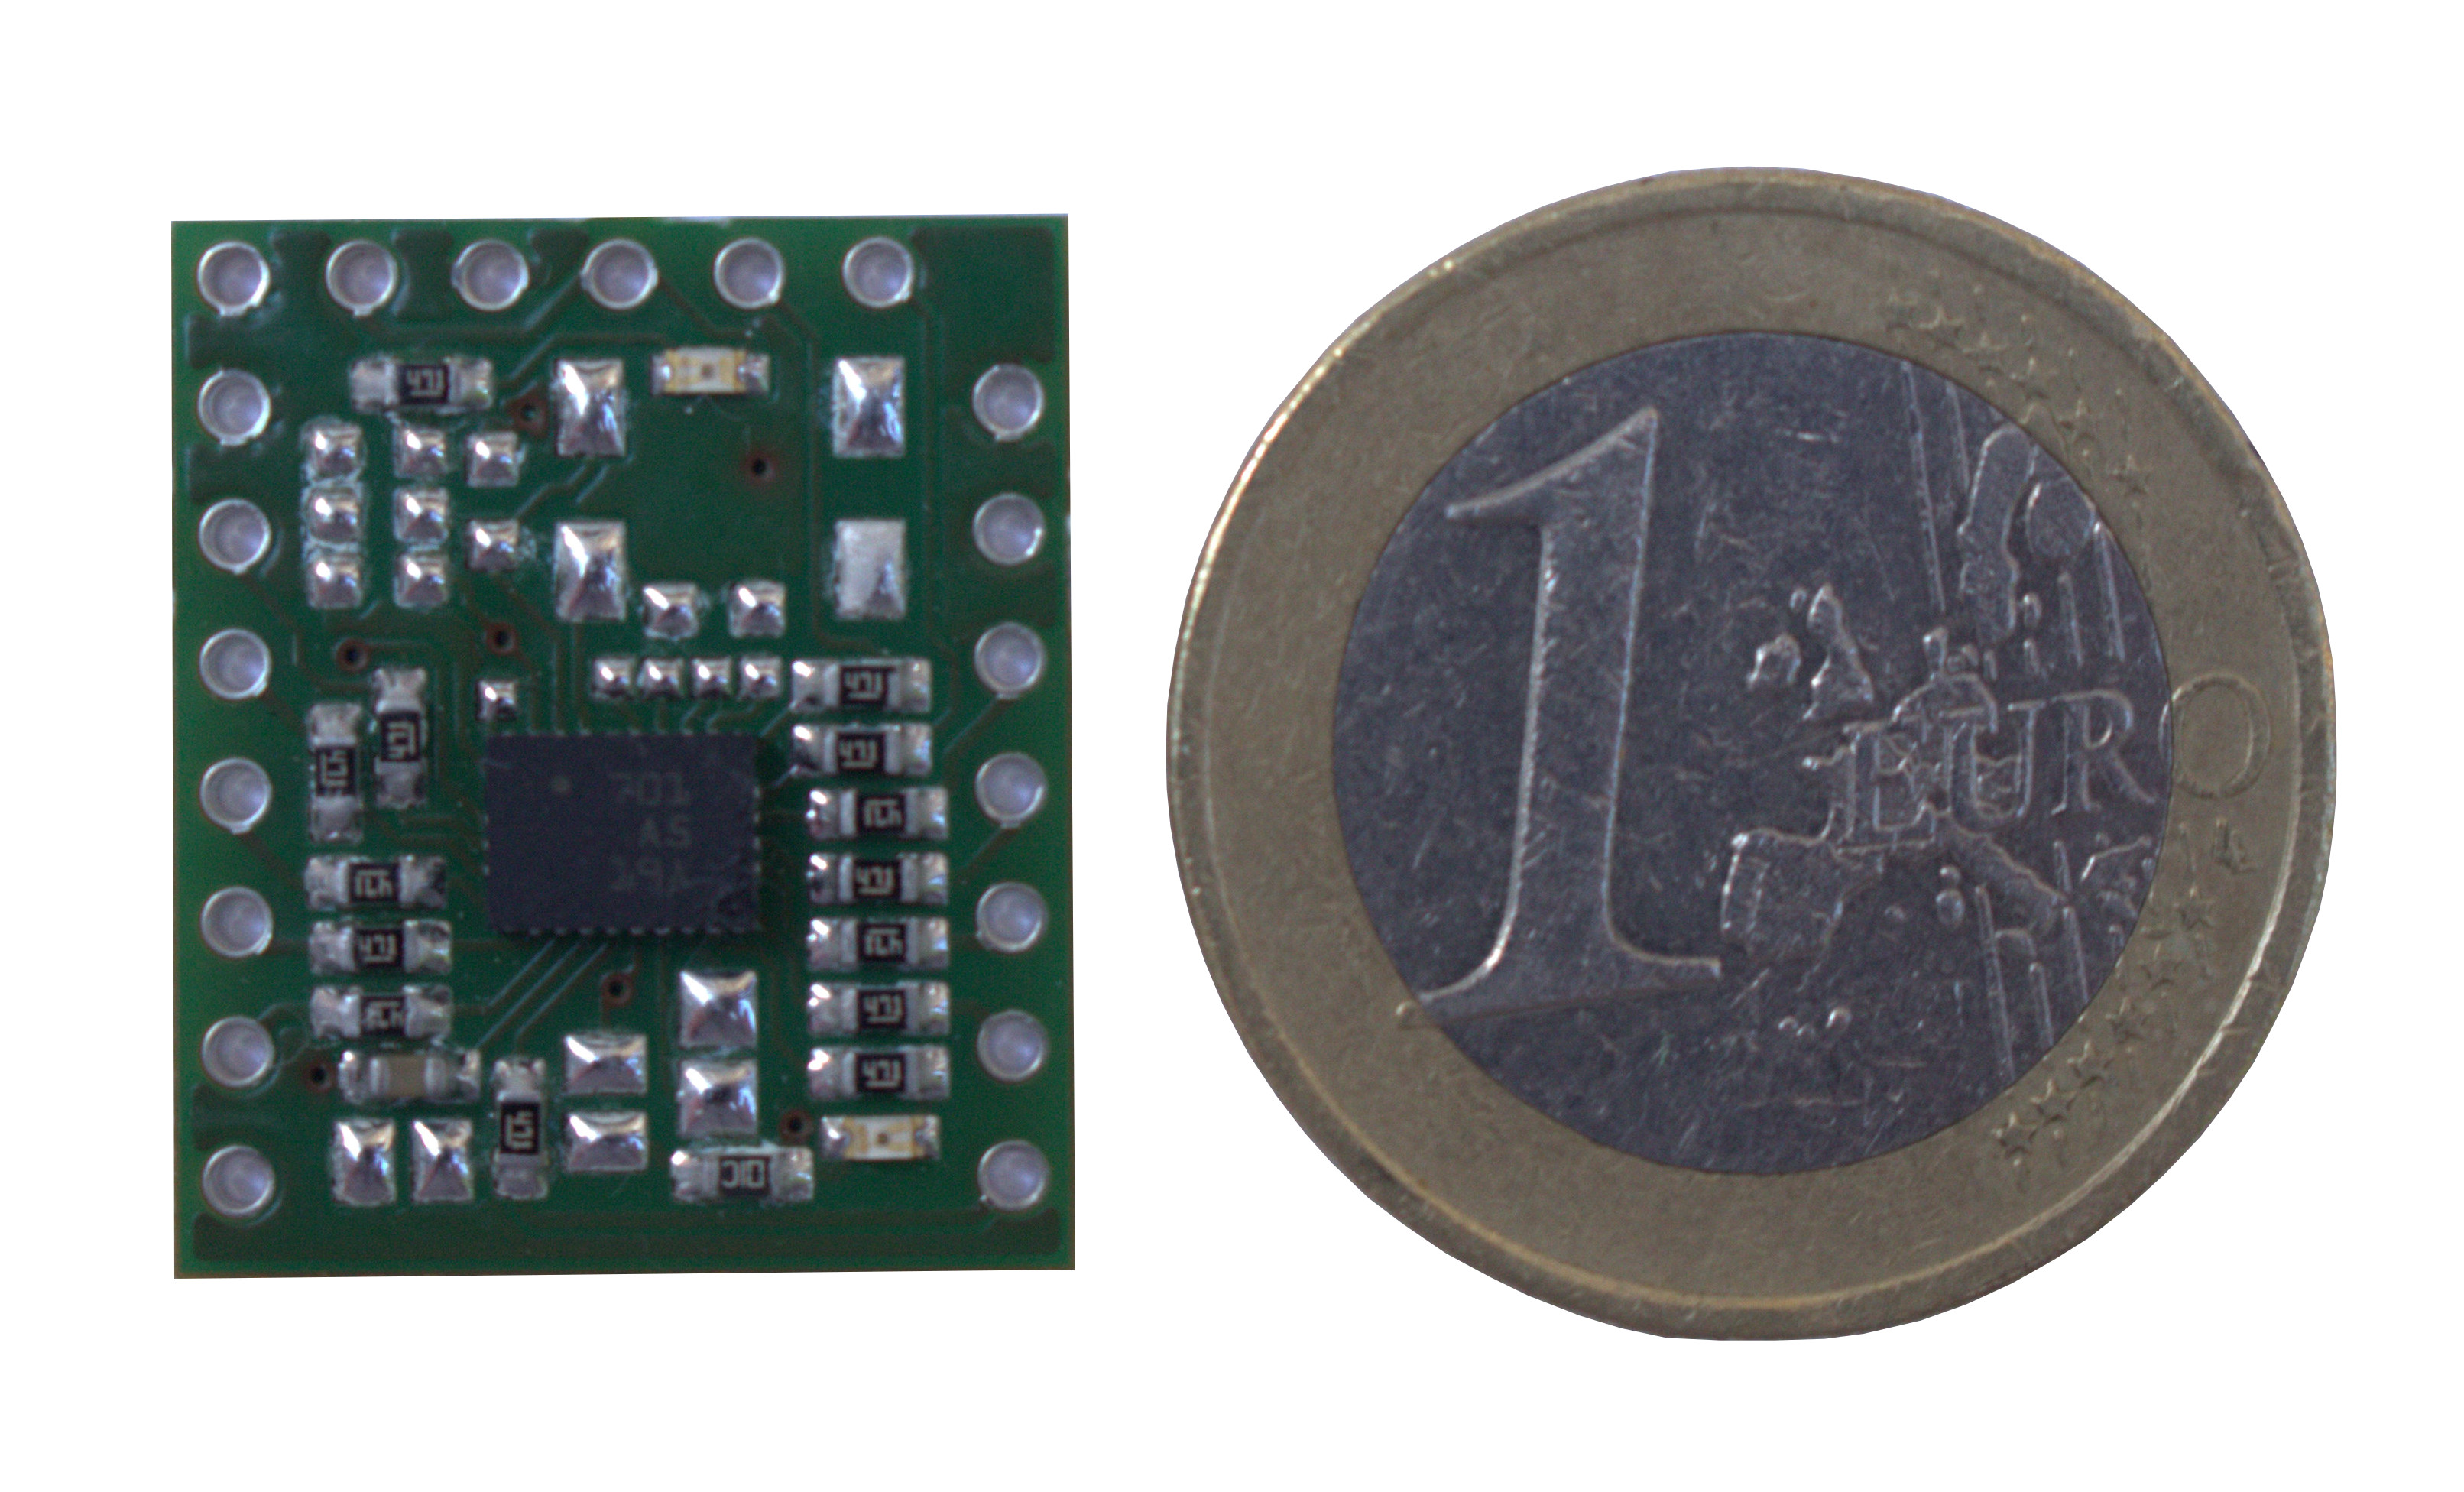
\includegraphics[width=7cm]{img/BMF055.jpg}
	\end{minipage}
	\vrule{}
	\begin{minipage}[c]{.45\textwidth}
		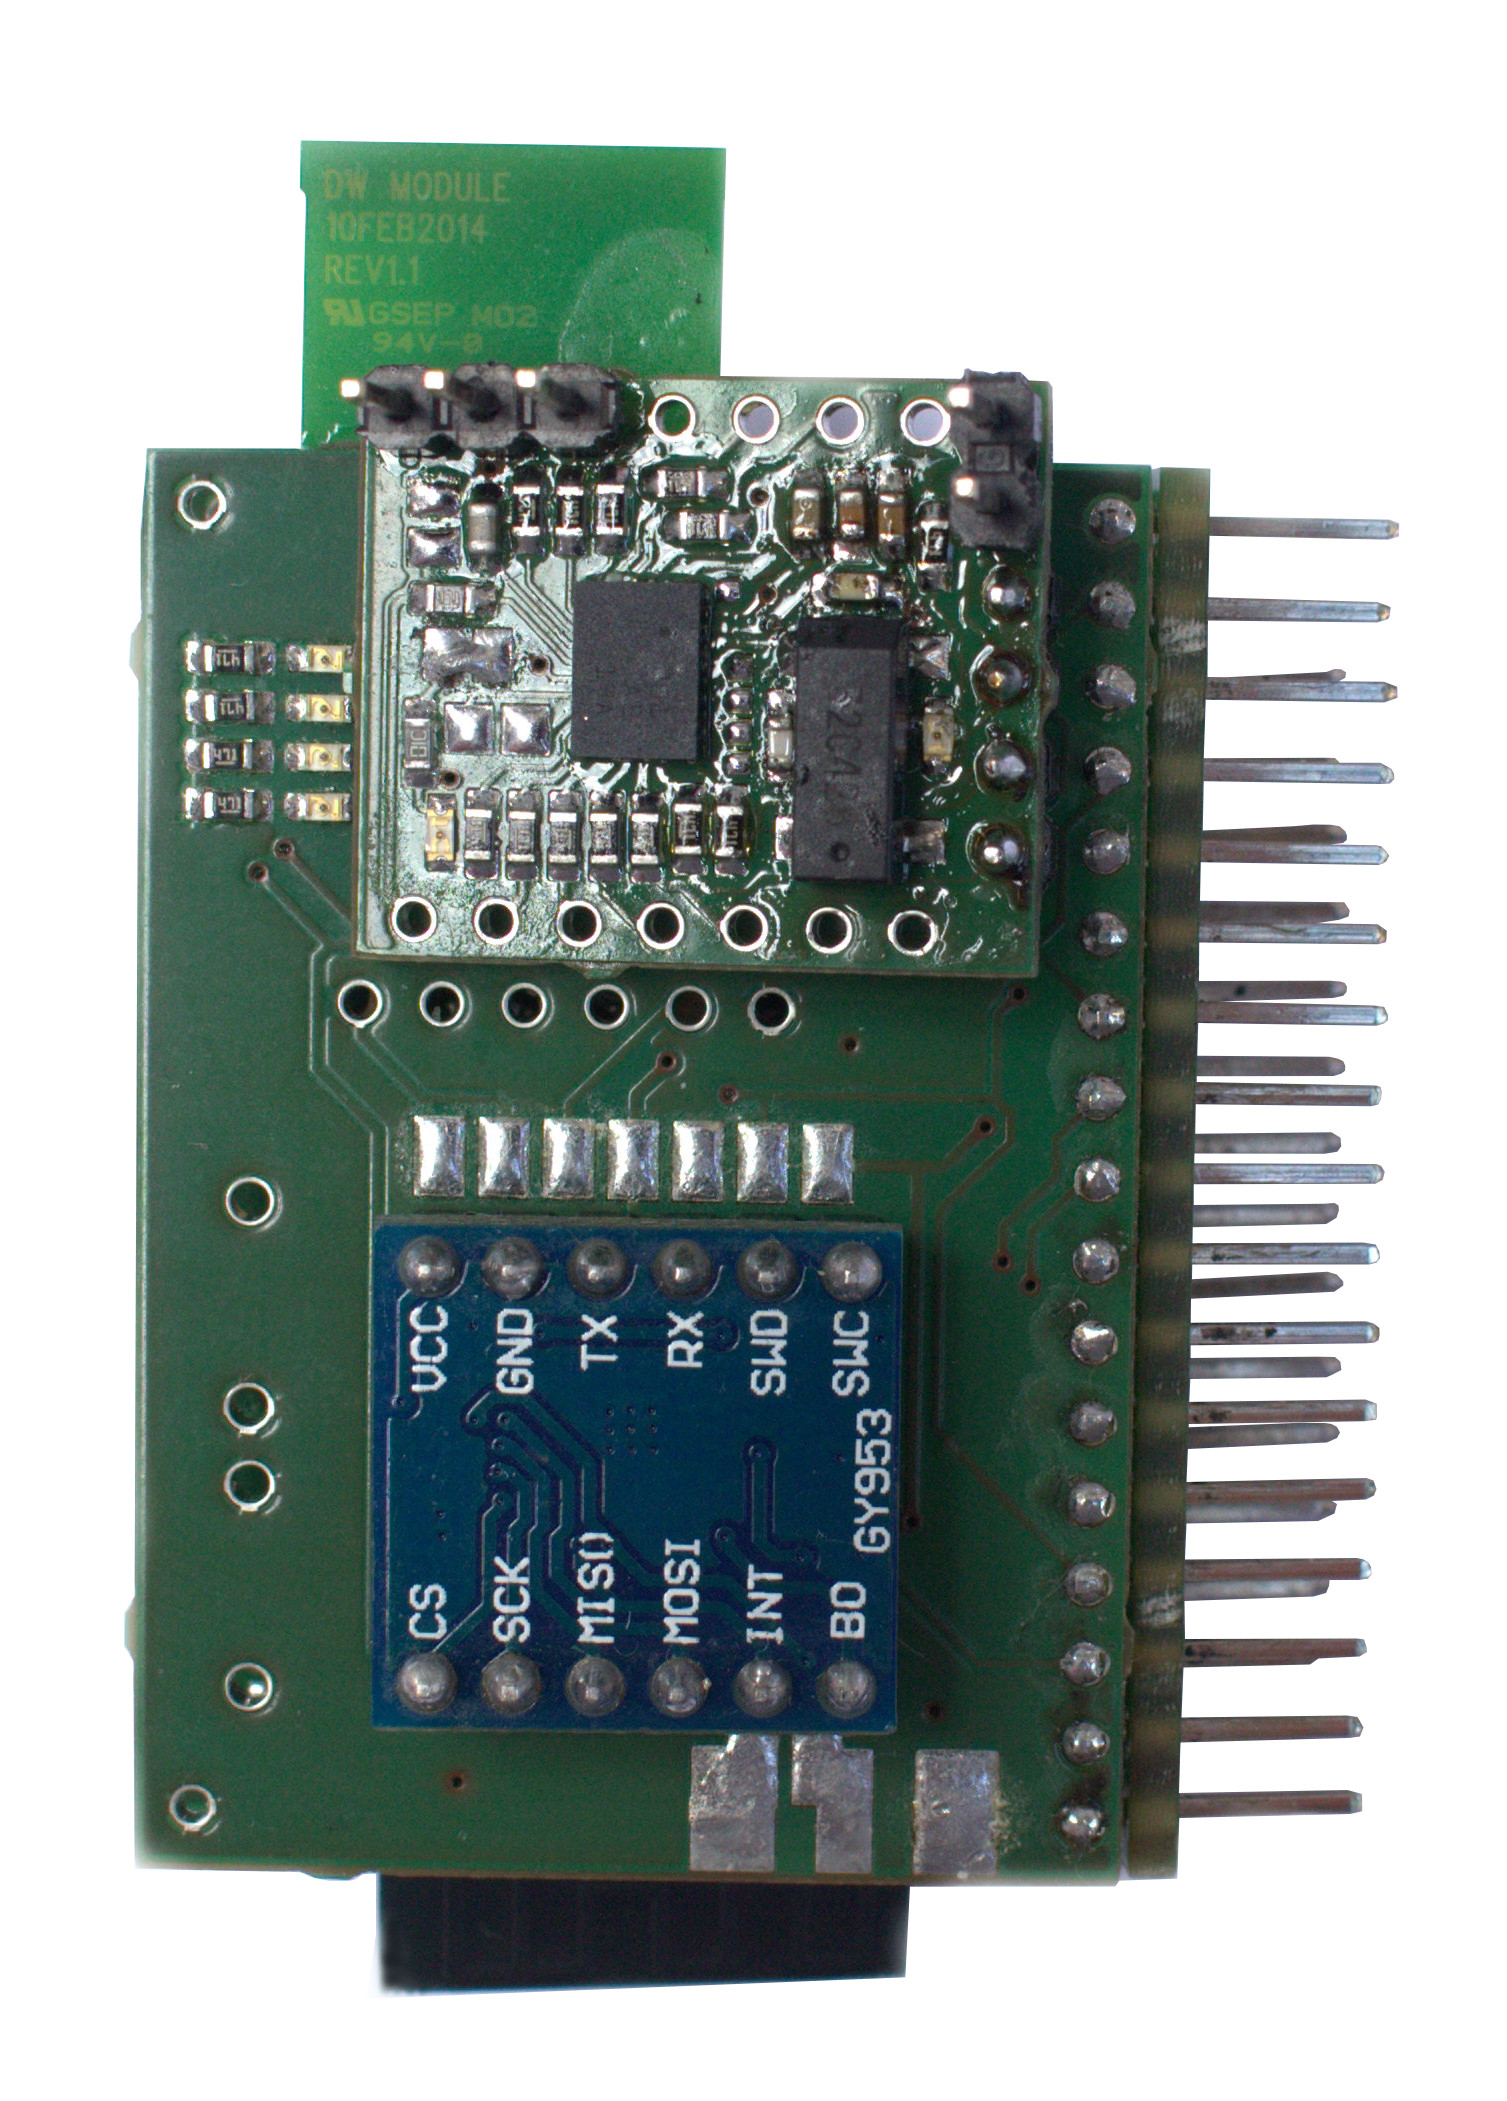
\includegraphics[width=7cm]{img/HWassembledNoCoin.jpg}
	\end{minipage}
\end{figure}

The BMF055 board has several usages because it contains a user programmable controller. It can be used for example as a simple UAV controller or autopilot. The project BMF055-flight-controller \cite{BMF055flightController} implemented this single chip autopilot solution for multicopters.

The Atmel SAM D20 controler \cite{atmel:samd20} can be programmed in Atmel Studio \cite{AtmelStudio} and the program can be flashed to the chip via \ac{SWD} interface \cite{SWDinterface}. We have to use Atmel ICE programmer \cite{AtmelICE} or similar hardware. For details about configuration and programming of the BMF055 chip we can follow the BMF055 datasheet \cite{bosch:BMF055} or the Atmel SAM D20 datasheet \cite{atmel:samd20}. The pinout of the BMF055 board and other hardware details are described in Appendix \ref{BMF055pinNumbering}. The figure \ref{BMF055AtmelStudio} shows an opened BMF055 project in Atmel Studio 7.

\begin{figure}
	\centering
	\label{BMF055AtmelStudio}
	\caption{An opened BMF055 project in Atmel Studio 7}
	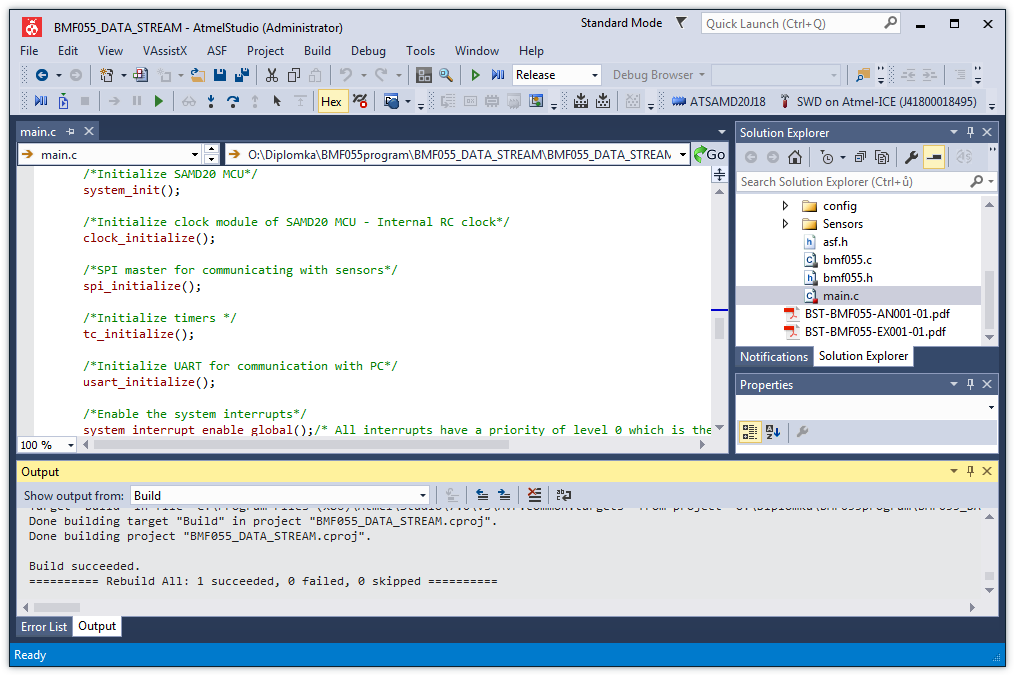
\includegraphics[width=\linewidth]{img/BMF055AtmelStudio.png}
\end{figure}

\section{Application Programming Interface}
The programming interface for the SensorBoard can be split into several categories. There is a native support from the manufacturer of the microcontrollers. This \ac{API} is written for any electronic device with the targeted microcontroller and this \ac{API} is mentioned in section \ref{GeneralAPI}.

I have implemented a new library for easier working with the sensors on the SensorBoard. This library is described in section \ref{SensorBoardAPI}.

\subsection{SensorBoard \ac{API}}
\label{SensorBoardAPI}
The ESP32 and Atmel SAM controller have defined their \ac{API} by the manufacturer, but these \ac{API}s don't implement a communication with specific sensors and peripherals connected to the controllers. For easier work with all the functionality of the SensorBoard, I have implemented specific \ac{API} for the ESP32 controller.

The \ac{API} is built on \ac{ESP-IDF} and it should be used together with the \ac{ESP-IDF} \ac{API} from the manufacturer. It allows, for example, a FreeRTOS usage, because the FreeRTOS is a part of \ac{ESP-IDF} framework \cite{ESP32}. The SensorBoard \ac{API} can be used together with Arduino \ac{API} for ESP32, too.

\paragraph{The SensorBoard \ac{API} implements}
\begin{itemize}
	\item Peripherials:
	\begin{itemize}
		\item \textbf{MPU9250} Accelerometer, dynamic gyroscope and magnetometer
		\item \textbf{BMP280} Barometer (Altitude meter)
		\item \textbf{Programmable LEDs} Two green LEDs
		\item \textbf{PWM Servo output} Controlling connected servos or regulators
		\item \textbf{File System} SD card and SPI file system
		\item \textbf{ADP5062} Battery charger and power supply configuration
		\item \textbf{Buttons} Read button state as input device
		\item \textbf{WiFi} Access Point, FTP server, remote control and communication protocol
	\end{itemize}
	\item Internal functionality:
	\begin{itemize}
		\item \textbf{Global Settings} Configuration file stored on the SD card
		\item \textbf{Stopwatch} Checking the timing of tasks
		\item \textbf{Test Sensor} Virtual sensor used for testing other functionalities
	\end{itemize}
	\item Partially implemented and actually unused
	\begin{itemize}
		\item \textbf{BMI160} Acclerometer and dynamic gyroscope
		\item \textbf{LTR-329ALS} Light sensor
		\item \textbf{SI7006} Humidity and teperature sensor
	\end{itemize}
\end{itemize}

The \ac{API} is documented in the source code and in the separate generated file.

\subsection{General \ac{API} for the controllers}
\label{GeneralAPI}
Both controllers used on the SensorBoard have an \ac{API} defined and implemented by the manufacturer.

\paragraph{Atmel SAM D21:} \cite{AtmelSAMd20API}
\begin{multicols}{2}
	\begin{flushleft}
		\begin{itemize}
			\setlength\itemsep{1pt}
			\item AC -- Analog Comparator (Callback \ac{API}s)
			\item ADC -- Analog-to-Digital Converter (Polled \ac{API}s)
			\item T30TSE75X Temperature Sensor
			\item AT45DBX DataFlash
			\item AVR2025 -- IEEE 802.15.4 MAC Stack v3.1.1
			\item AVR2025 -- TAL
			\item AVR2025 -- TFA
			\item AVR2025-MAC Serial Interface Module
			\item AVR2130 -- LW MESH v1.2.1
			\item BOD -- Brown Out Detector
			\item CRC-32 calculation
			\item CRC32 -- 32-bit cyclic redundancy check
			\item DAC -- Digital-to-Analog Converter (Callback \ac{API}s)
			\item Debug Print (FreeRTOS)
			\item Delay routines
			\item EEPROM Emulator Service
			\item Ethernet Physical Transceiver (ksz8851snl)
			\item EVSYS -- Event System with interupt hooks support
			\item EXTINT -- External Interrupt (Polled \ac{API}s)
			\item FatFS file system
			\item Generic board support
			\item GFX Monochrome -- Menu System
			\item GFX Monochrome -- Monochrome Graphic Library
			\item GFX Monochrome -- Spinner/Spin control widget
			\item GFX Monochrome -- System Font
			\item Interrupt management -- SAM implementation
			\item IOPORT -- General purpose I/O service
			\item Memory Control Access Interface
			\item NVM -- Non-Volatile Memory
			\item PAC -- Peripheral Access Controller
			\item Performance Analyzer Application
			\item PORT -- GPIO Pin Control
			\item QTouch Library for SAMD20/D21
			\item RTC -- Real Time Counter in Calendar Mode (Callback \ac{API}s)
			\item RTC -- Real Time Counter in Count Mode (Callback \ac{API}s)
			\item SAM D20/D21 implementation of AT25DFx SerialFlash with vectored master SPI
			\item SD/MMC stack on SPI interface
			\item SERCOM I2C -- Slave Mode I2C (Polled \ac{API}s)
			\item SERCOM SPI -- Serial Peripheral Interface (Callback \ac{API}s)
			\item SERCOM SPI -- Serial Peripheral Interface (Master Mode, Vectored I/O)
			\item SERCOM USART -- Serial Communications (Polled \ac{API}s)
			\item Serial I/O -- Host using UART
			\item Serial I/O -- NCP Using UART
			\item Sleep manager -- SAMD implementation
			\item Smart Card
			\item SSD1306 OLED controller
			\item Standard serial I/O (stdio)
			\item SYSTEM -- Clock Management for SAMD20
			\item SYSTEM -- I/O Pin Multiplexer
			\item TC -- Timer Counter (Callback \ac{API}s)
			\item Unit test framework -- SAM0 implementation
			\item USART -- Serial interface -- SAM implementation for devices with only USART
			\item WDT -- Watchdog Timer (Polled \ac{API}s)
		\end{itemize}
	\end{flushleft}
\end{multicols}

\paragraph{Espressif ESP-WROOM-32:} \cite{ESP32API}
\begin{multicols}{2}
	\begin{itemize}
		\item Wi-Fi
		\begin{itemize}
			\setlength\itemsep{1pt}
			\item Wi-Fi
			\item Smart Config
			\item ESPNOW
		\end{itemize}
		\item Mesh
		\begin{itemize}
			\setlength\itemsep{1pt}
			\item ESP Mesh
		\end{itemize}
		\item Bluetooth
		\begin{itemize}
			\setlength\itemsep{1pt}
			\item Bluetooth Controller \&\& VHCI
			\item Bluetooth Common
			\item Bluetooth LE
			\item Bluetooth Classic
		\end{itemize}
		\item Ethernet
		\begin{itemize}
			\setlength\itemsep{1pt}
			\item Ethernet
		\end{itemize}
		\item Peripherals
		\begin{itemize}
			\setlength\itemsep{1pt}
			\item ADC
			\item DAC
			\item GPIO (including RTC low power I/O)
			\item I2C
			\item I2S
			\item LED Control
			\item MCPWM
			\item Pulse Counter
			\item Remote Control
			\item SDMMC Host
			\item SD SPI Host
			\item Sigma-delta Modulation
			\item SPI Master
			\item SPI Slave
			\item Timer
			\item Touch Sensor
			\item UART
		\end{itemize}
		\item Protocols
		\begin{itemize}
			\setlength\itemsep{1pt}
			\item mDNS
			\item ESP-TLS
		\end{itemize}
		\item Storage
		\begin{itemize}
			\setlength\itemsep{1pt}
			\item SPI Flash and Partition \ac{API}s
			\item SD/SDIO/MMC Driver
			\item Non-Volatile Storage
			\item Virtual Filesystem
			\item FAT Filesystem
			\item Wear Levelling
			\item SPIFFS Filesystem
		\end{itemize}
		\item System
		\begin{itemize}
			\setlength\itemsep{1pt}
			\item FreeRTOS
			\item FreeRTOS Hooks
			\item Heap Memory Allocation
			\item Heap Memory Debugging
			\item Interrupt Allocation
			\item Watchdogs
			\item Inter-Processor Call
			\item High Resolution Timer
			\item Logging
			\item Application Level Tracing
			\item Power Management
			\item Sleep Modes
			\item Base MAC address
			\item Over The Air Updates (OTA)
			\item ESP pthread
		\end{itemize}
		\item Configuration Options
		\begin{itemize}
			\setlength\itemsep{1pt}
			\item Kconfig
		\end{itemize}
	\end{itemize}
\end{multicols}

\section{Usage Examples}
The SensorBoard is a multifunctional user programmable hardware that can be used in several ways. There are some examples presented in this section.

\subsection{Sensors data logger}
\label{ExampleLogger}
Sensor logger can be understood as very simple logging device or as a very advanced application with an integrated web server and with the ability to connect more boards into one synchronized grid with centralized control. The simple version is shown in figure \ref{UELogging1ELogging1}.

\begin{figure}
	\centering
	\label{UELogging1}
	\caption{Simple logging application with SensorBoard}
	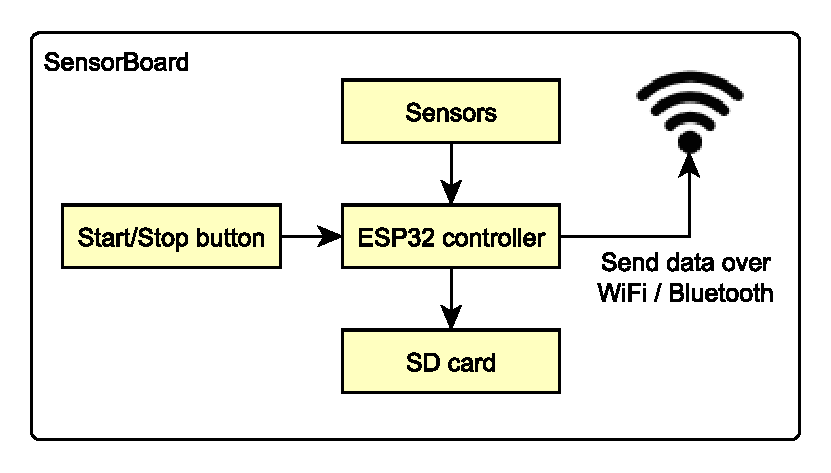
\includegraphics[scale=1]{img/UsageExamplesLogger1.pdf}
\end{figure}

When we need to measure some inertial data, we sometimes need more sensors placed in different places. Then, it's a big advantage when we can start and stop all the sensors synchronously and control all of them by one button. This solution is shown in figure \ref{UELogging2}.

\begin{figure}
	\centering
	\label{UELogging2}
	\caption{Advanced logging application with SensorBoard}
	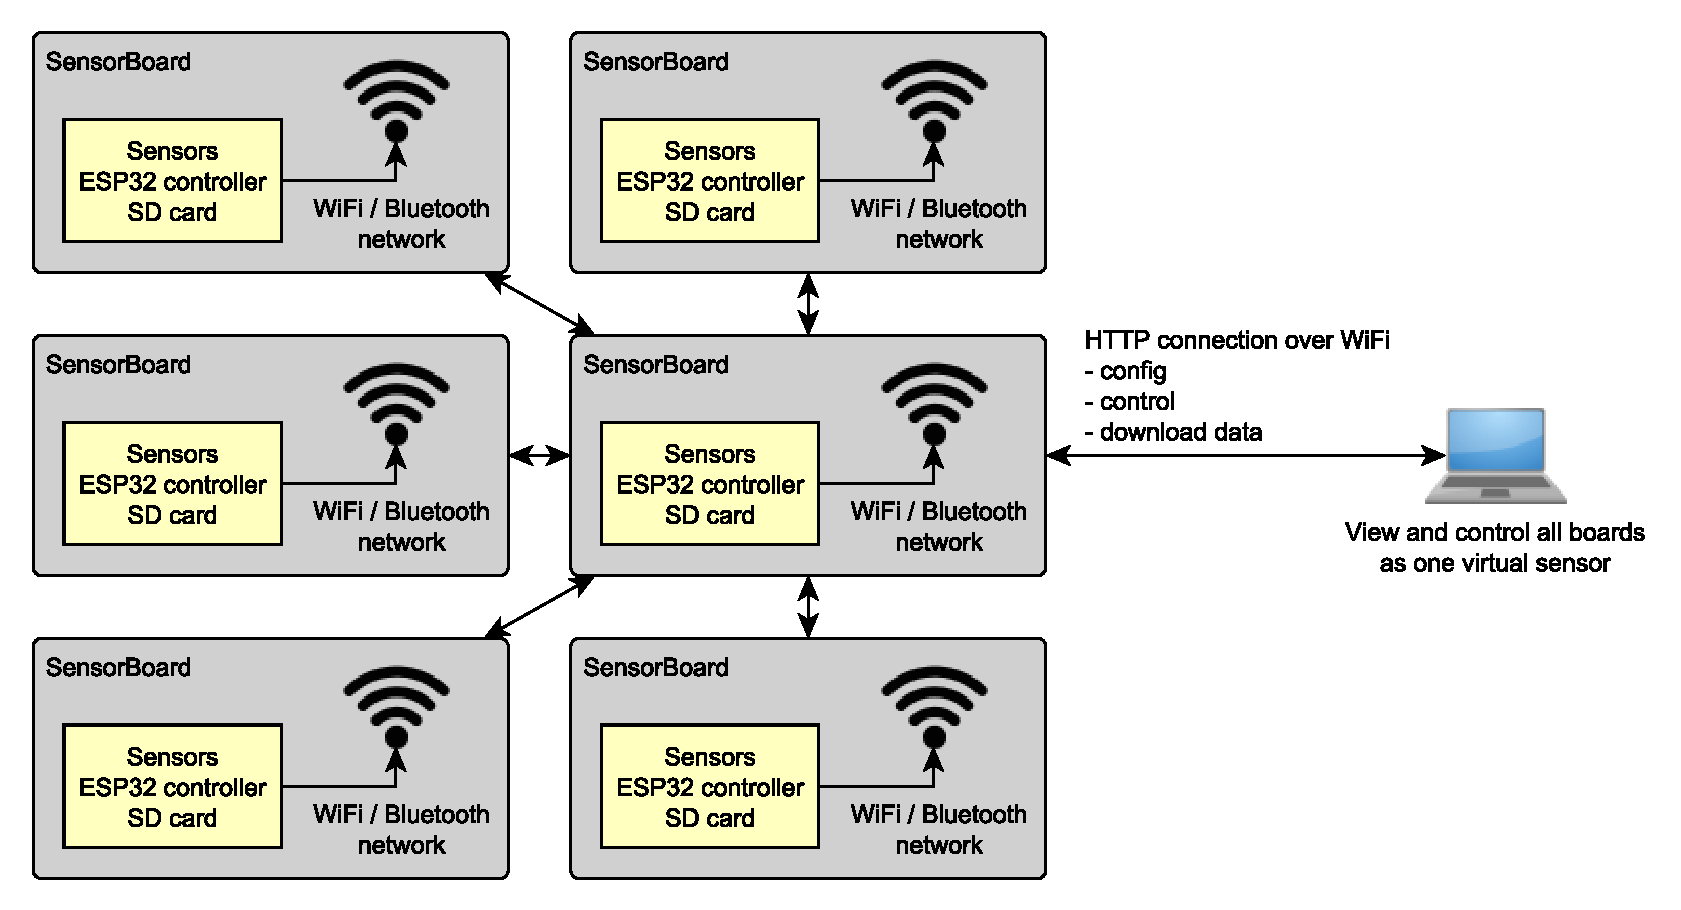
\includegraphics[width=\linewidth]{img/UsageExamplesLogger2.pdf}
\end{figure}

I'm using this advanced configuration during the analysis of a movement of a horse. This solution is explained in detail in section \ref{HorseFirmware}. The goal of this task is to recognize the type of the movement of a horse (stand, walk, trot or gallop). So, we can get some results from only one sensor, but we get better results when we can measure each leg and the body separately. How the SensorBoards are used in this task is shown in figure \ref{UELoggingHorse}.

\begin{figure}
	\centering
	\label{UELoggingHorse}
	\caption{Configuration of the SensorBoards during measurement of a movement of a horse}
	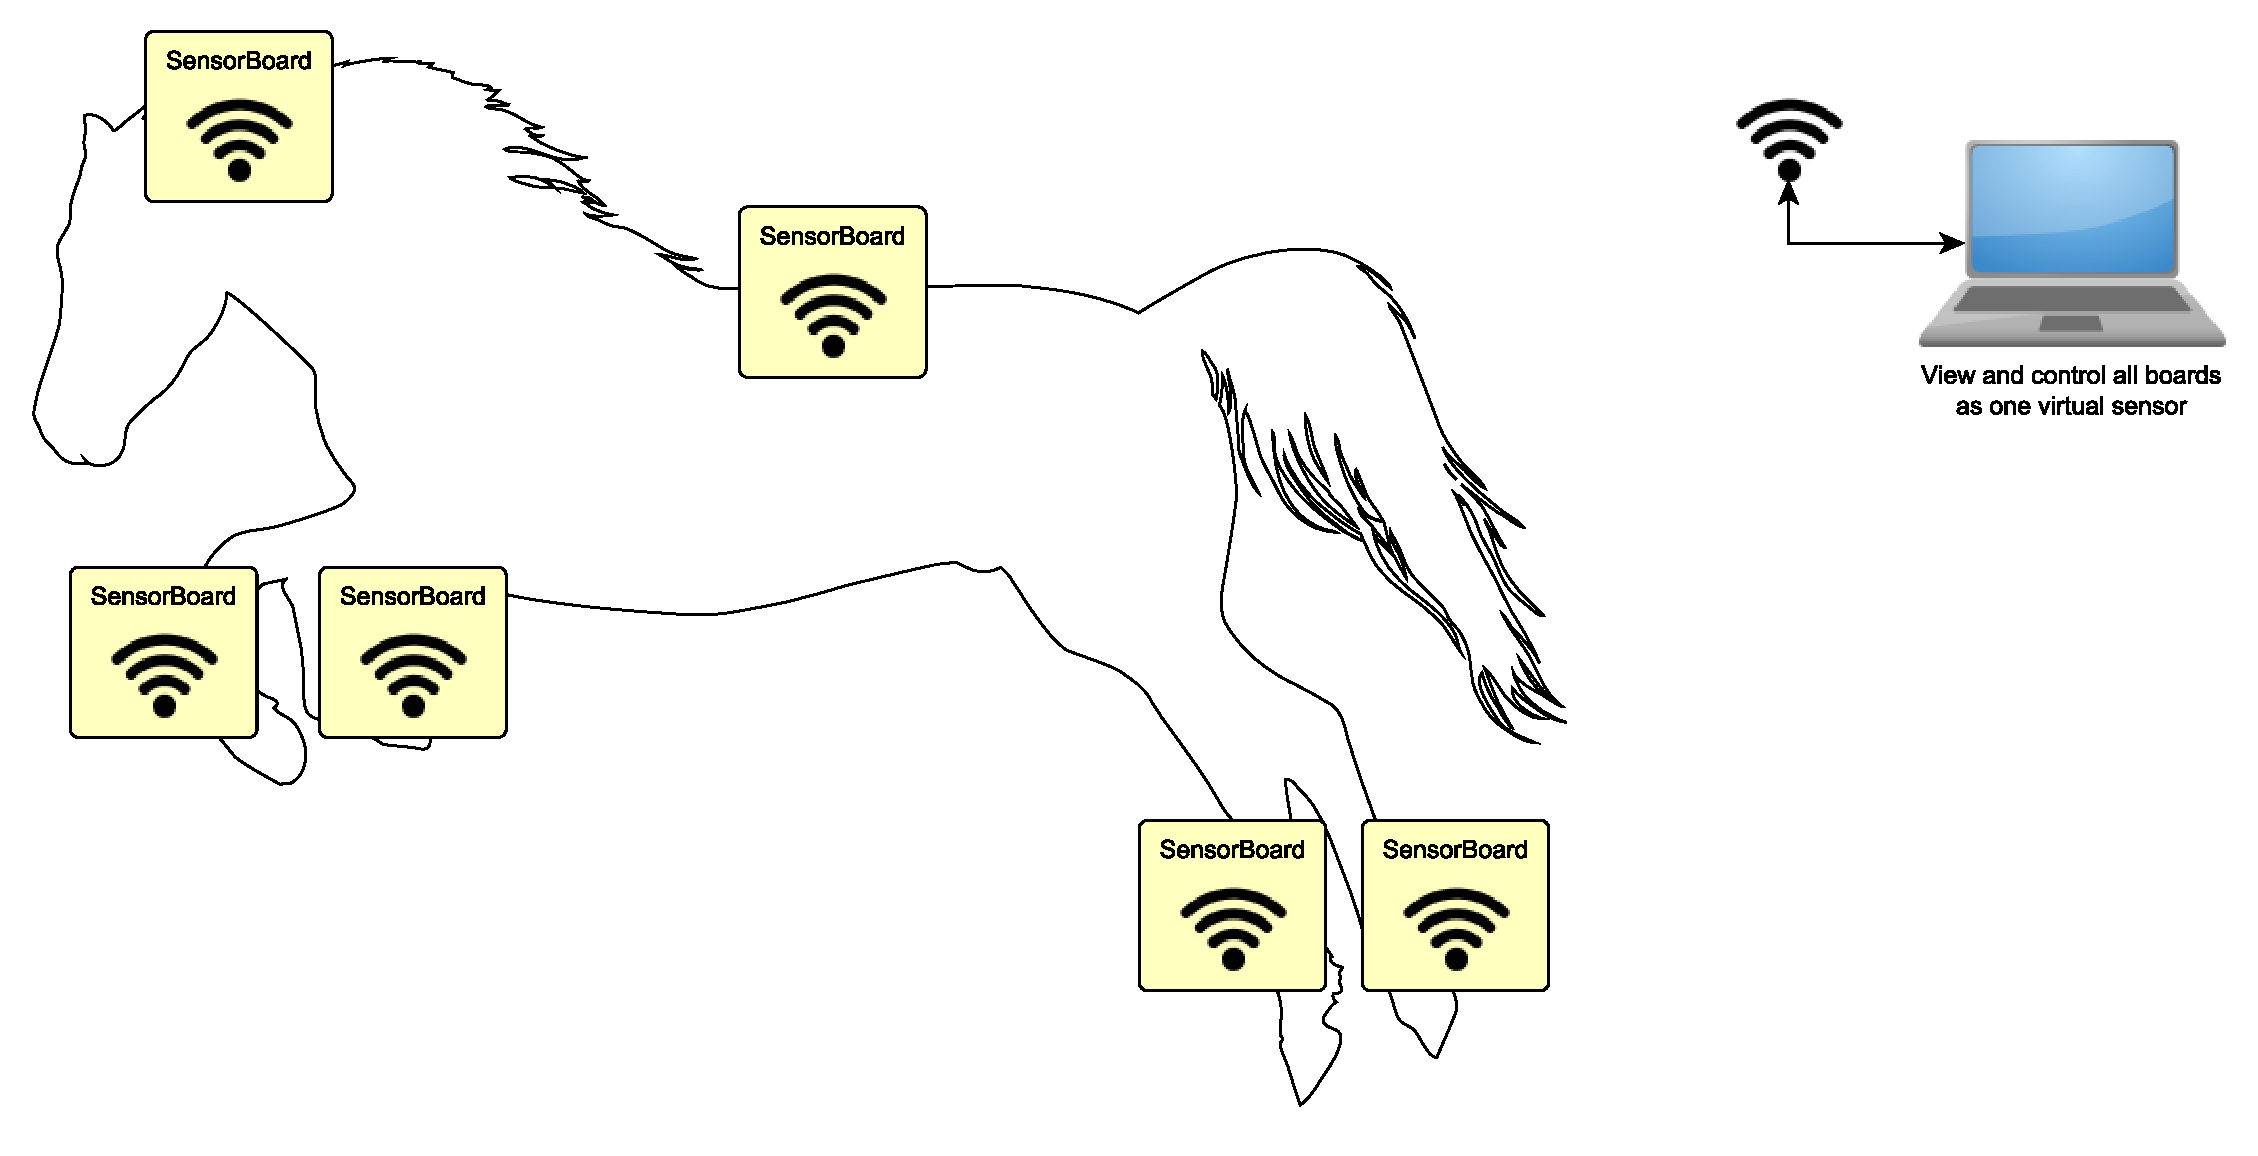
\includegraphics[width=\linewidth]{img/UsageExamplesLoggerHorse.pdf}
\end{figure}

\subsection{Sensor fusion and \ac{AHRS}}
\label{ExampleAHRS}
Sensor fusion is a method that combines data from more sensors and calculates new information. The new information is read from the sensor fusion algorithm like from a virtual sensor. \cite{SensorFusion}

This example shows how to use a sensor fusion algorithm to computing \ac{AHRS} data on the SensorBoard. \ac{AHRS} is Attitude and heading reference system and computes pitch, roll and yaw values from triaxial accelerometer, dynamic gyroscope and magnetometer data. We can use for example Madgwick's algorithm \cite{MadgwickAHRS} in the way shown in figure \ref{UEAHRS}. This application is a base step for example \ref{ExampleBMF055FlightController}.

\begin{figure}
	\centering
	\label{UEAHRS}
	\caption{Sensor fusion example on custom \ac{AHRS}}
	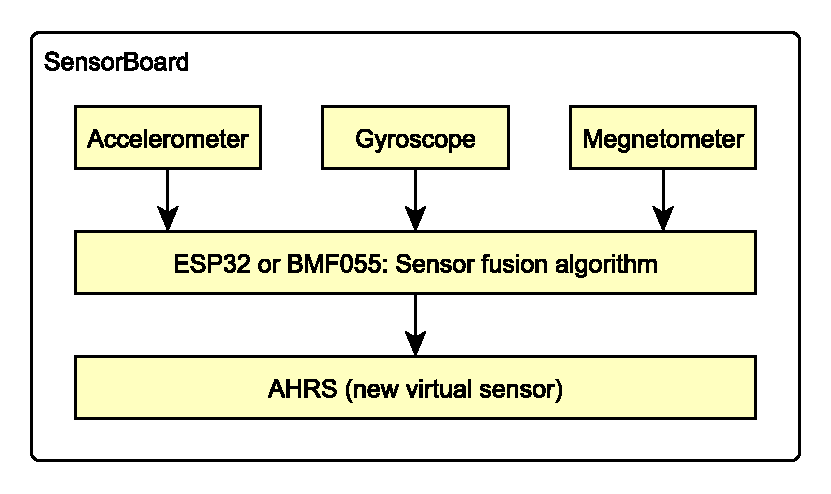
\includegraphics[scale=1]{img/UsageExamplesAHRS.pdf}
\end{figure}

We can use an advantage of two controllers at one board and run the sensor fusion algorithm on the BMF055 chip and the ESP32 is still free for some user program like is shown in figure \ref{UEAHRSBMF}. When an error occurs in the user program, the sensor fusion at BMF055 chip continues to run without any problem. This feature is a big advantage for Flight Controllers where we want to allow the user to run for example his navigation code.

\begin{figure}
	\centering
	\label{UEAHRSBMF}
	\caption{Sensor fusion \ac{AHRS} example with two controllers}
	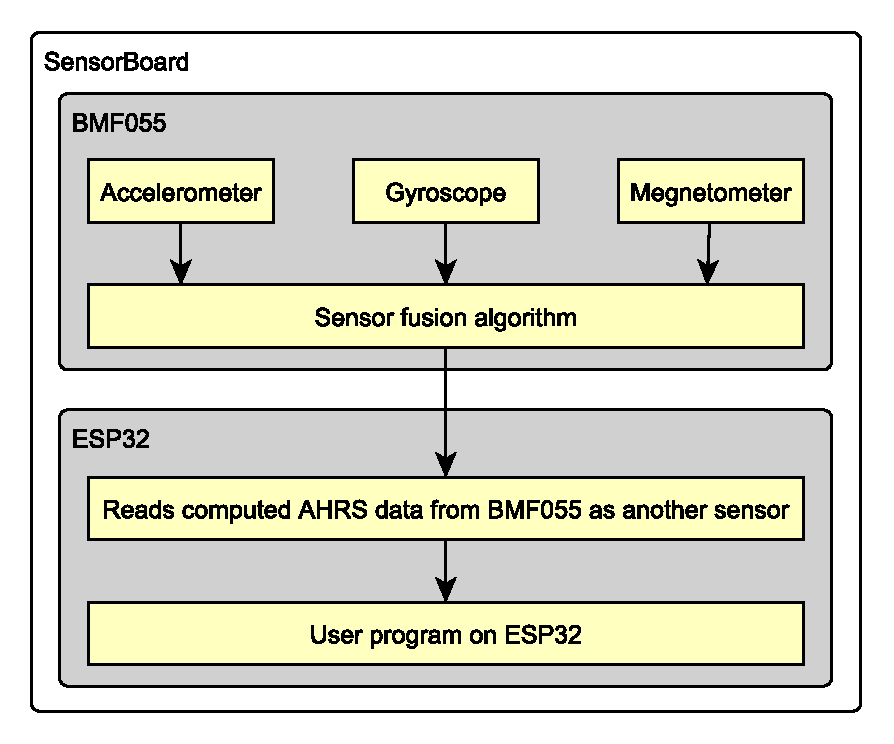
\includegraphics[scale=1]{img/UsageExamplesAHRSBMF.pdf}
\end{figure}

\subsection{UAV Flight controller with non-critical user programmable processor}
\label{ExampleBMF055FlightController}
The flight controllers must be very reliable devices. They usually consist of two parts. The first part controls the pitch, roll, yaw, velocity, the angle of attack etc. The second part is a navigator that processes user commands and makes high-level flight planning. The pilot's input can be processed on both parts. We usually want to create only the basic control algorithm, which is safety critical and develop all the remaining as a non-critical code.

Here we can use dual controller advantage on the SensorBoard and run the basic critical code at the first controller and the remaining non-critical code on the second controller. The non-critical program on the second controller is usually a navigator or user program. The figure \ref{UEFlightController} shows the possible configuration of the flight controller on the SensorBoard. This configuration uses BMF055 Flight Controller \cite{BMF055flightController} by Lukas Blocher. His code can be compiled directly for the SensorBoard without any modification.

\begin{figure}
	\centering
	\label{UEFlightController}
	\caption{SensorBoard used as a quadcopter flight controller}
	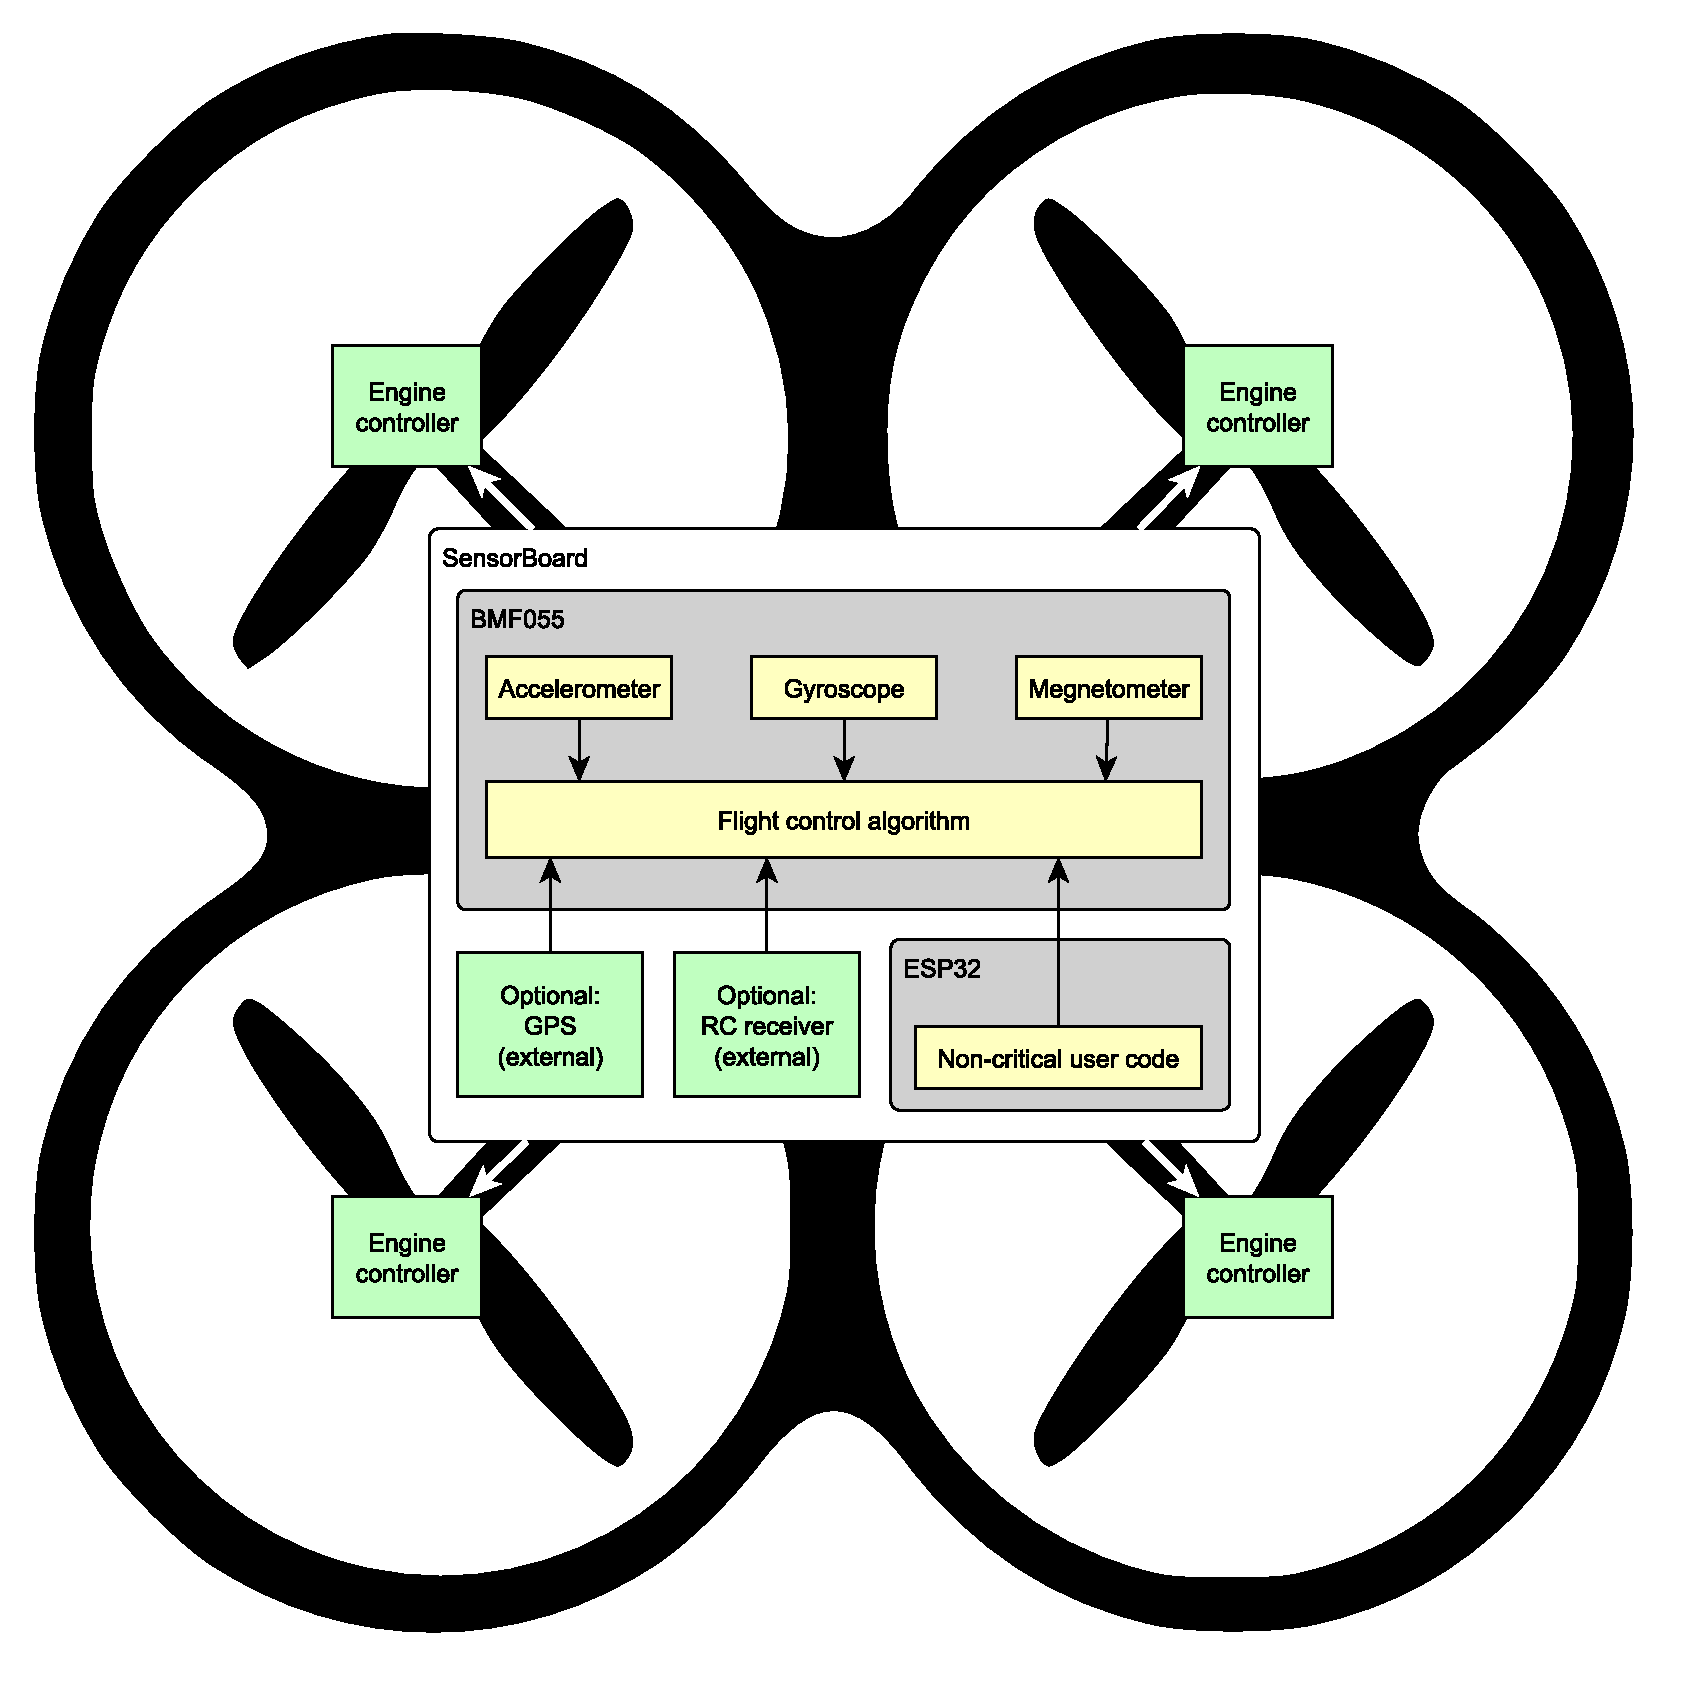
\includegraphics[width=\linewidth]{img/UsageExamplesFlightController.pdf}
\end{figure}

\subsection{Indoor navigation using \ac{TDOA}}
Indoor navigation requires high accuracy positioning. We usually need higher accuracy than given by GPS. I know so many projects approaching the indoor positioning. There was, for example, an Indoor Positioning and Indoor Navigation conference in September 2017 in Japan.

This example uses Time Difference of Arrival (\ac{TDOA}) method to compute its position in space with the precision of \SI{10}{cm}. The device measures time differences in received messages from other devices. When the device knows the time differences and the speed of light, it can compute its relative position to the other boards. There is a DWM1000 chip that is able to measure and compute these data. \cite{decawave:DWM1000}. The figure \ref{UEETDOA} shows how the relative positioning works on the SensorBoard.

\begin{figure}
	\centering
	\label{UETDOA}
	\caption{\ac{TDOA} relative location service on the SensorBoard}
	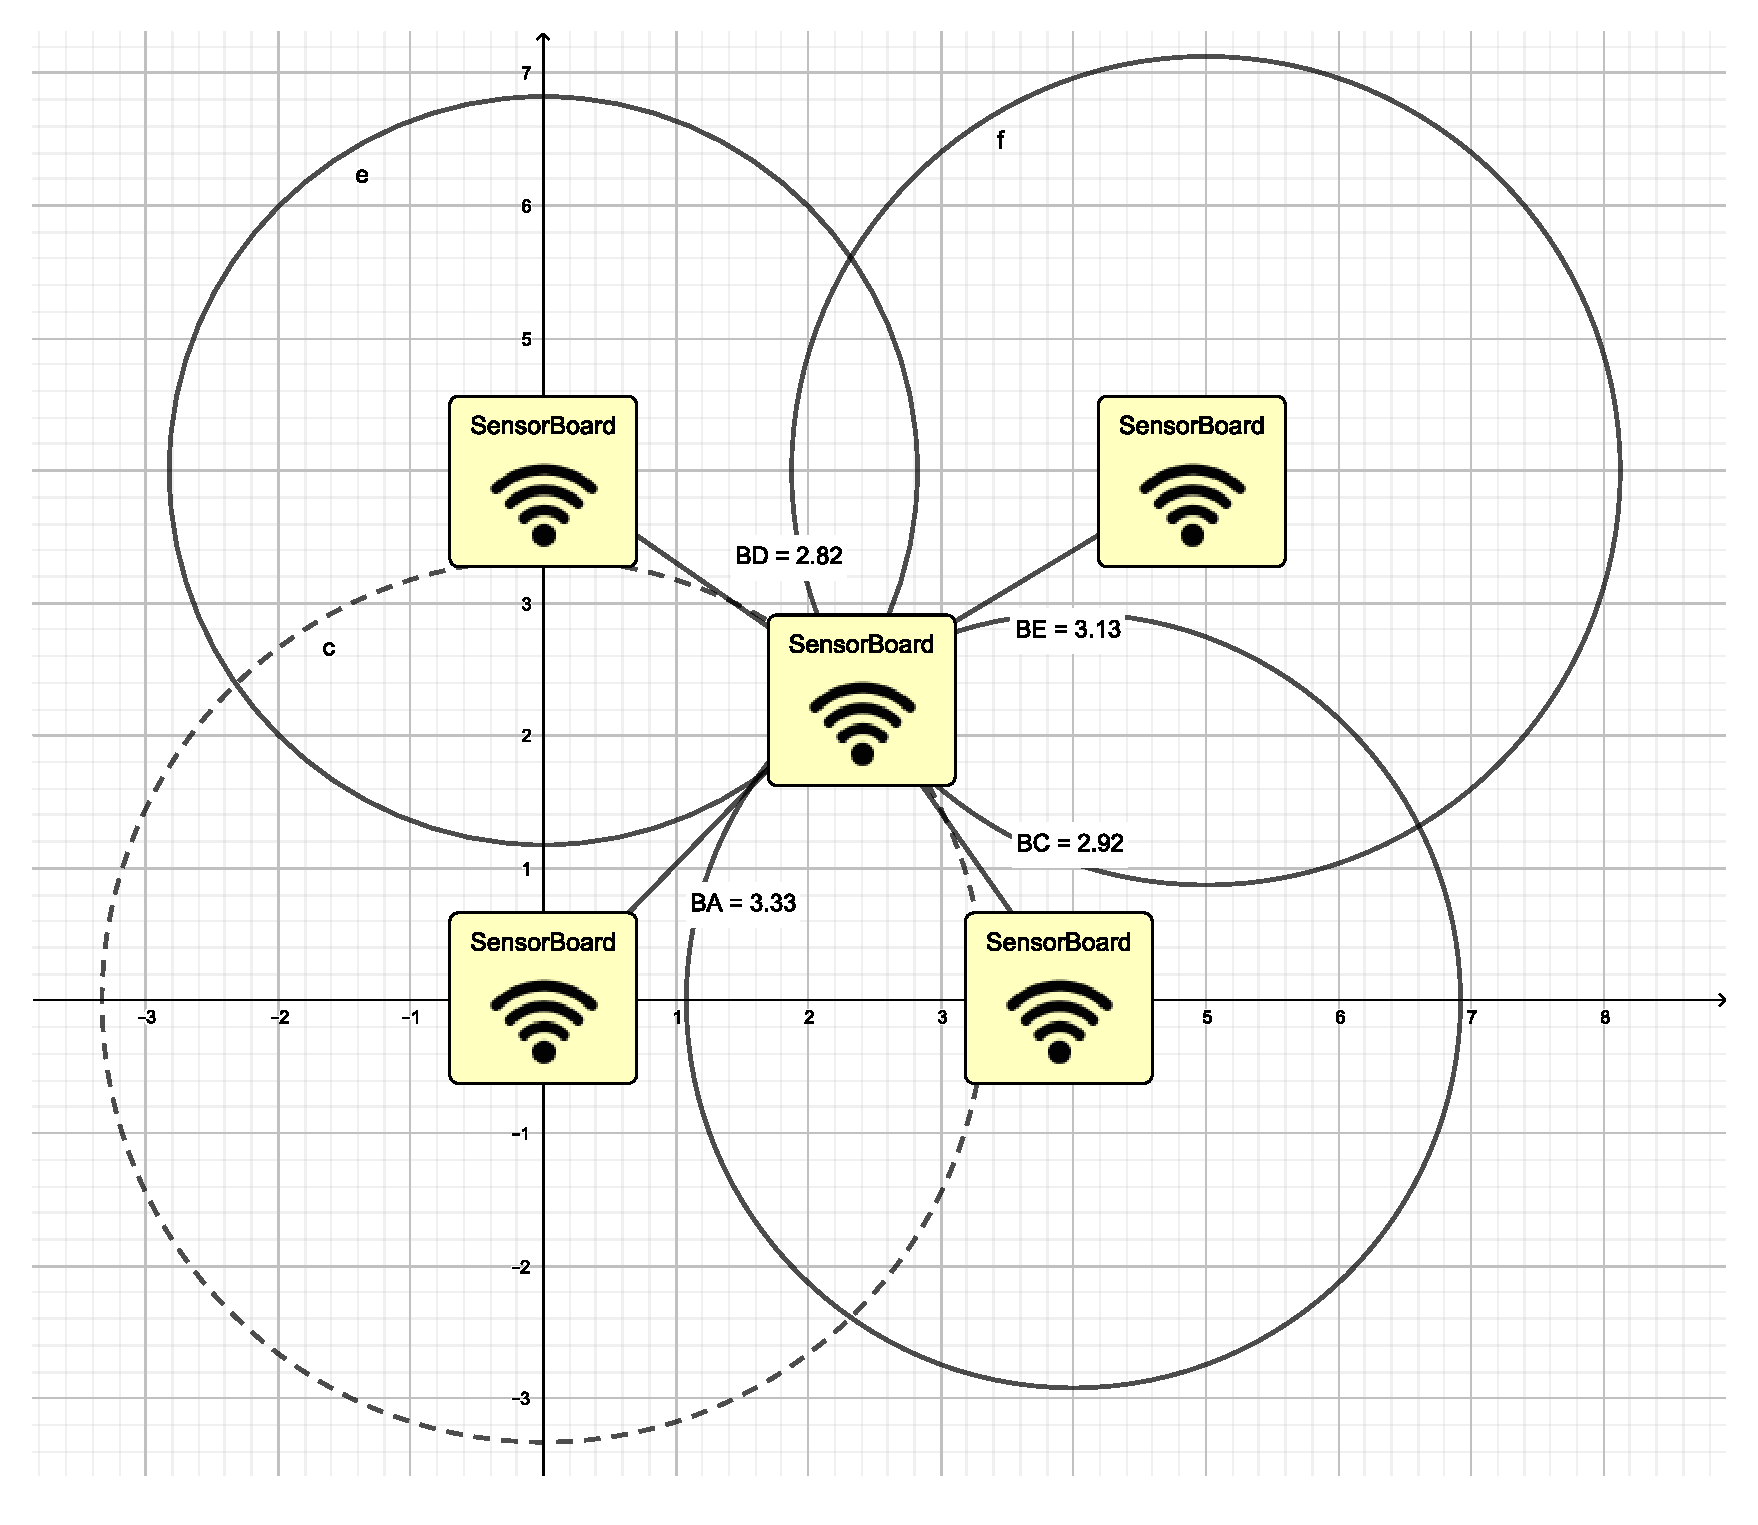
\includegraphics[trim=5cm 6cm 5cm 5cm, clip, width=15cm]{img/UsageExamplesTDOA.pdf}
\end{figure}

The DWM1000 \cite{decawave:DWM1000} module is present on SensorBoard and when it connects to at least three other boards, then it computes its relative position with the mentioned precision. When the board knows an absolute position of the other boards, it can compute its absolute position, too. The absolute location can be obtained for example from GPS receiver or from static transmitters.

When we use the \ac{AHRS} mentioned in section \ref{ExampleAHRS}, we have all data about current position and attitude of the SensorBoard. We can use some other sensors on the SensorBoard like BMP280 barometer \cite{bosch:BMP280} to improve the current position and attitude data.

\subsection{RTOS education board}
Real-time systems are different from common operating systems in personal computers and they cannot be emulated as a standard application for a computer with the common operating system. The common operating system doesn't give a guarantee that a job completes on time, so any application running on this operating system cannot give this guarantee, too.

The ESP32 controller on the SensorBoard uses FreeRTOS and supports all its functionality. \cite{ESP32FreeRTOS} So, we can run a hard real-time system on the SensorBoard or on the other hand, we can use the SensorBoard for education about real-time systems. Simple FreeRTOS application uses only the ESP32 controller like is shown in figure \ref{UEFreeRTOS} and optionally we can use the sensors as data sources and as resources.

\begin{figure}
	\centering
	\label{UEFreeRTOS}
	\caption{FreeRTOS application diagram on ESP32 on the SensorBoard}
	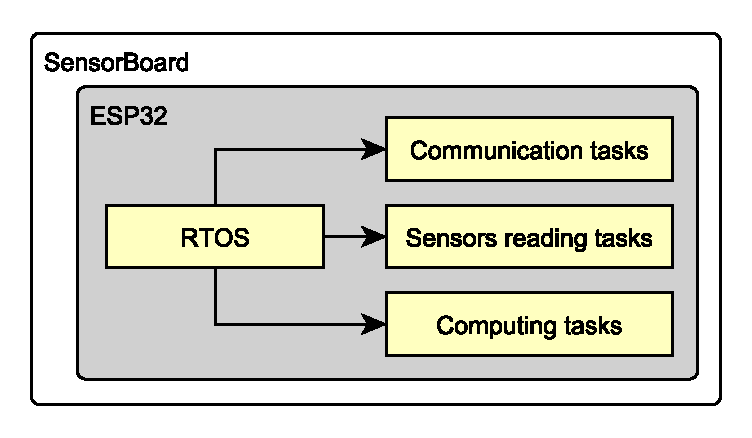
\includegraphics[scale=1]{img/UsageExamplesRTOS.pdf}
\end{figure}

\subsection{MicroPython Robot Controller}
The SensorBoard supports MicroPython firmware \cite{MicroPython} on the ESP32 controller. When we create a Python library that implements simple \ac{API} for controlling some electromechanical device. We can use the SensorBoard as a controller of this electromechanical hardware. Then we simply send Python commands via UART or WiFi to the target device.

In my opinion, this setup is an easy way how to teach the basics of programming (in Python) with some dynamic hardware. This way of teaching is probably easier for the students and it probably creates more interactivity between students and the device. The figure \ref{UEMicroPython} shown an example of using MicroPython inside the SensorBoard.

\begin{figure}
	\centering
	\label{UEMicroPython}
	\caption{MicroPython robot controller example on the SensorBoard}
	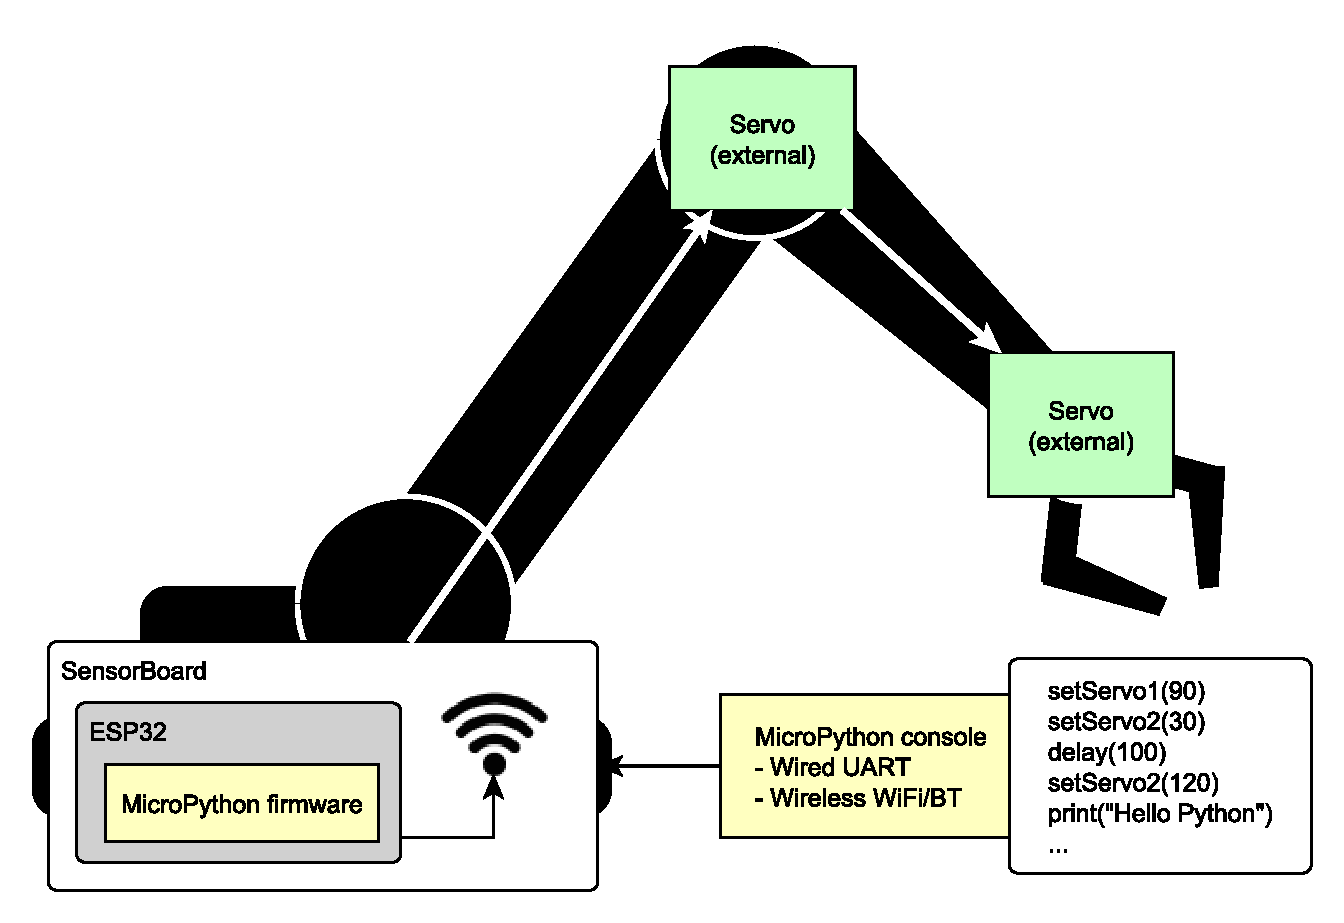
\includegraphics[width=\linewidth]{img/UsageExamplesPythonRobot.pdf}
\end{figure}

\subsection{WiFi AccessPoint with server services}
The ESP32 controller has a built-in Bluetooth and WiFi module. So, we can create any WiFi based application on the SensorBoard. The only limitation is memory (SD card up to \SI{32}{GB}) and CPU power (dual-core \SI{240}{MHz}). We can use the SensorBoard for example as a simple HTTP server \cite{ESP32:HTTPserver} or FTP server \cite{ESP32:FTPserver} or implement any other WiFi-based service like is shown in figure{UEWiFi}.

\begin{figure}
	\centering
	\label{UEWiFi}
	\caption{WiFi based services example on the SensorBoard}
	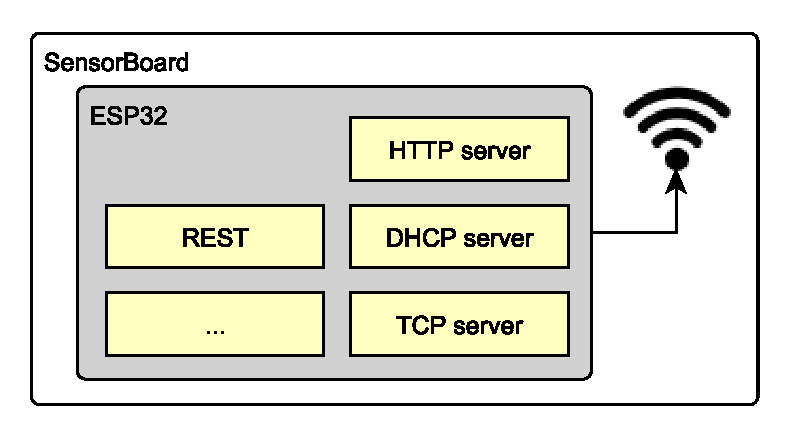
\includegraphics[scale=1]{img/UsageExamplesServer.pdf}
\end{figure}

\subsection{Grid computing education board}
\label{ExampleGrid}
The biggest advantages of the SensorBoard are hidden in its real-time system, wireless technology and independence. These advantages can create a grid of multiple items. Then we can use the whole grid as one virtual unit. When we solve the problems with failures and accessibility, we have a grid solution with swappable items. An example of a grid with two failures is shown in figure \ref{UEEgrid}.

\begin{figure}
	\centering
	\label{UEgrid}
	\caption{Example of a grid with two failures created from multiple SensorBoards}
	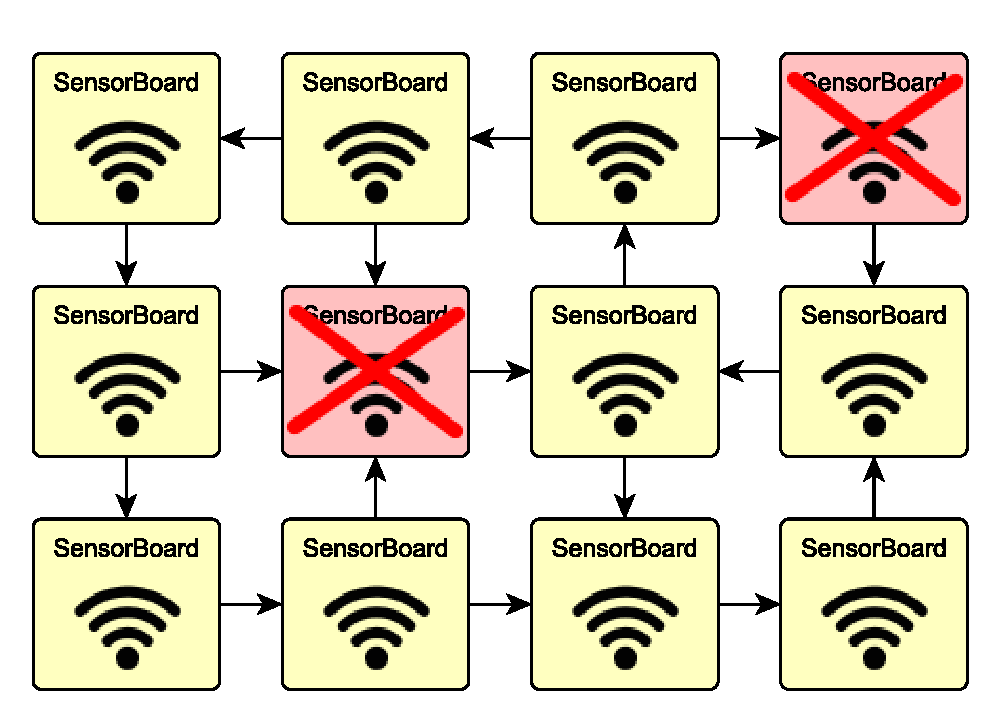
\includegraphics[width=\linewidth]{img/UsageExamplesGrid.pdf}
\end{figure}

\subsection{\ac{IoT} wireless sensors}
The Internet of Things (\ac{IoT}) is a commercially used word for all devices connected to the Internet with some sensors onboard. The SensorBoard fulfills both conditions and it can be used directly this way. The figure \ref{UEIoT} shows an example of using the SensorBoard as a device reading sensors data and streaming them via GSM network or via WiFi connection.

\begin{figure}
	\centering
	\label{UEIoT}
	\caption{Example of using SensorBoard as an \ac{IoT} device streaming data from sensors via WiFi or GSM network}
	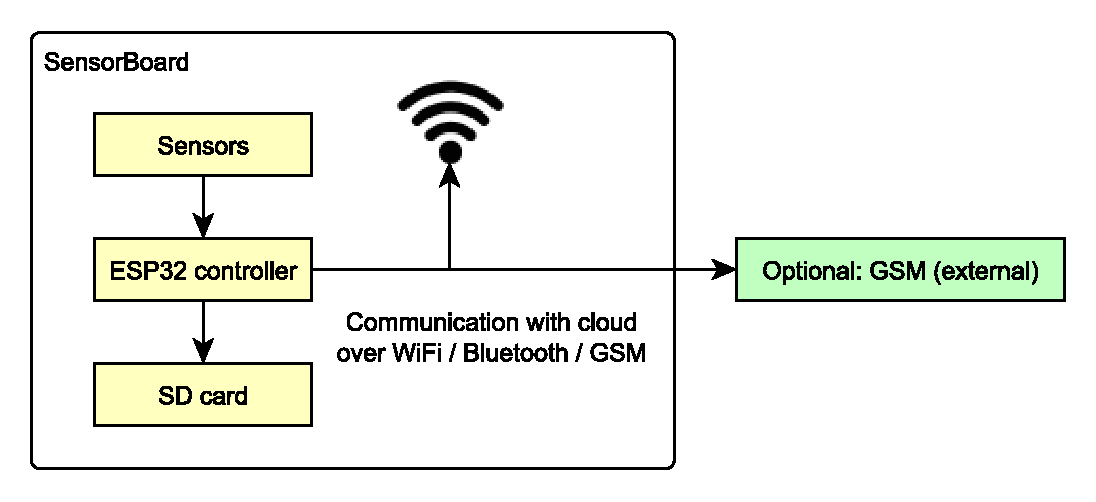
\includegraphics[width=\linewidth]{img/UsageExamplesIoT.pdf}
\end{figure}

\section{Movement Analysis Firmware}
\label{HorseFirmware}
The firmware is a sensor data logging application similar to the example in section \ref{ExampleLogger}. The program is able to read values from sensors in a defined frequency and store the captured data to SD card and/or send them directly via WiFi. The application is controlled by start/stop button or via \ac{TCP} connection.

When the SensorBoard is switched on, it initializes WiFi access point and waits 5 seconds before the reading and logging procedure starts. After these 5 seconds, the board enters a loop and starts logging data to SD card. The logging loop can be stopped via \ac{TCP} connection, by pressing the start/stop button or by switching the board off.

When we want to control the SensorBoard via \ac{TCP} client, we have to connect our device to SensorBoard's WiFi access point. Then we can connect to the \ac{TCP} server and send the control commands.

\subsection{Before first use}
\label{beforeFirstUse}
All the configuration is saved in \texttt{config.ini} file on the SD card (root directory). The configuration is read every time when the SensorBoard is powered on. The configuration file is never modified by the SensorBoard. An example of the configuration file is in figure \ref{SBconfigFile}. If no configuration file is present on the SD card, default values are used.

\begin{figure}
	\centering
	\label{SBconfigFile}
	\caption{Example of the configuration file on SD card}
	\begin{verbatim}
	% Enable or disable WiFi adapter
	isWiFienabled = true
	
	% Initializes WiFi as an access point when true, otherwise as a station
	isWiFiAccessPoint = true
	
	% Network SSID
	% When initialized as a station: tries to connect
	% to an existing network with this SSID
	% When initialized as AP: creates the new network
	WiFiSSID = SensorBoard
	
	% WiFi network password
	WiFiPassword = 1234567890
	
	% IP address of the device,
	% if initialized as an access point, we can use 192.168.1.1
	myIP = 192.168.1.1
	
	% TCP server port
	TCPseverPort = 3000
	
	% If enabled, starts logging automatically 'startUpWaitTime' seconds
	% after powered on
	startLoggingImmediately = true
	
	% Waits N milliseconds before entering the logging loop
	startUpWaitTime = 5000
	
	% If enabled, the horse movement analysis starts automatically
	isHorseAnalysis = false
	
	% If enabled, the data streaming starts automatically
	isStreaming = false
	
	% If enabled, the logging can be controlled by the start/stop button
	isStartButtonUsed = false
	
	% Log file name for sensor data, a number prefix is automatically added
	logFileName = log.csv
	
	% Log file name for movement analysis,
	% a number prefix is automatically added
	horseAnalysisFileName = horse.txt
	\end{verbatim}
\end{figure}

\subsection{Files on the SD card}
All the files are stored and read from the root directory of the SD card. The files are:

\begin{itemize}
	\item \textbf{config.ini}: (read-only) Configuration file explained in section \ref{beforeFirstUse}.
	\item \textbf{counter.txt}: (read/write) This text file contains only one integer on the first line, other data are ignored. The SensorBoard has no real-time clock reference, so it cannot add a timestamp to each log file. The board increments this number after each startup. This number is used as session number of each log file.
	\item \textbf{X\_Y\_log.csv}: (write only) The main log file in CSV format. The name consists of the session number \texttt{X}, log number \texttt{Y} and the configured filename. The format is \texttt{X\_Y\_NAME}, for example \texttt{12\_34\_log.csv}. It means, that the file was created after 12th switching on, it is 34th log during the session and the configured file name is \texttt{log.csv}.
	\item \textbf{format.txt} (write only) Format of the CSV main log file. This file contains names of all columns in order in the main log file. Example of this file is shown in figure \ref{formatFile}.
	\item \textbf{X\_Y\_horse.txt}: (write only) The movement analysis log file in plain text or CSV format. The \texttt{X}, \texttt{Y} numbers correspond to the main log file numbers. The files with the same numbers were captured simultaneously during the same measurement.
\end{itemize}

\begin{figure}
	\centering
	\label{formatFile}
	\caption{Example of the 'format.txt' file on SD card.}
	\begin{verbatim}
	'S'; #; milliseconds; baroAltitude QFE [m]; baroTemp [degree C];  \
	ACC_X [g]; ACC_Y [g]; ACC_Z [g];                                  \
	GYR_X [rad/s]; GYR_Y [rad/s]; GYR_Z [rad/s];                      \
	MAG_X [degree];  MAG_Y [degree];  MAG_Z [degree];                 \
	...
	\end{verbatim}
\end{figure}

\subsection{Using the firmware}
The application is usually used only during the measurement process. The behavior of the program can be described using the state machine presented in figure \ref{firmwareStateMachine}.

\begin{figure}
	\centering
	\label{firmwareStateMachine}
	\caption{State machine of the firmware}
	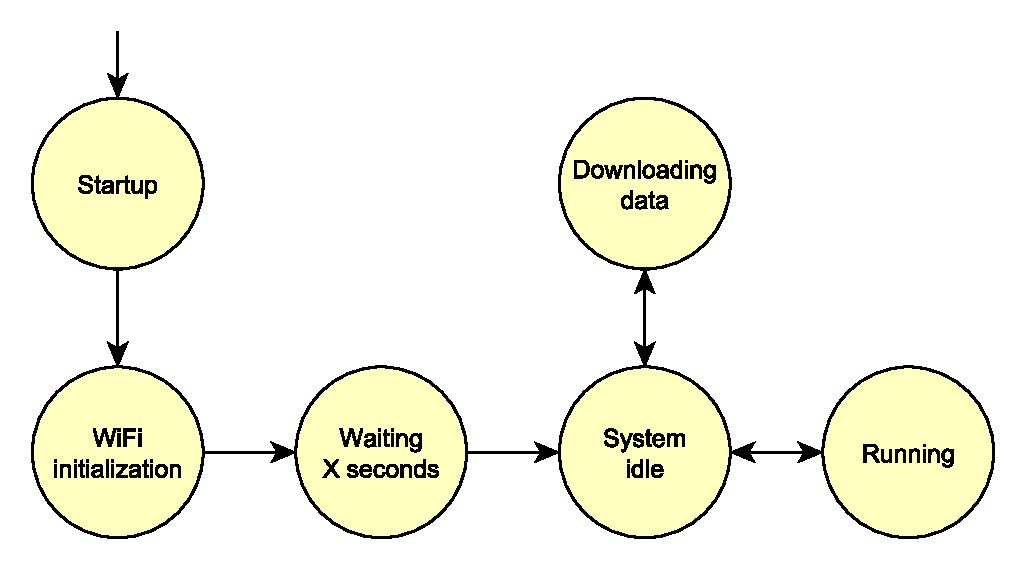
\includegraphics[width=\linewidth]{img/firmwareStateMachine.pdf}
\end{figure}

The meaning of each state of the machine:
\begin{itemize}
	\item \textbf{Startup} Powering on the board
	\item \textbf{WiFi initialization} Initialization of the WiFi adapter according to the configuration file
	\item \textbf{Waiting N seconds} Waiting a few (milli)seconds according to the configuration file. We usually configure this waiting when we want to prevent the creation of very short logs.
	\item \textbf{System idle} The system is waiting for control commands. If the board is configured to start logging immediately, the system automatically switches to running state.
	\item \textbf{Downloading data} The data can be downloaded directly from the SD card or to a connected device.
	\item \textbf{Running} The Running state starts the measuring loop and allows to log, stream or analyze the measured data. It's not possible to download data from SD card in this state. This state is activated when the user starts logging, streaming or movement analysis process from the Idle state. The Running state can be activated automatically according to the configuration file.
\end{itemize}

\subsection{Horse movement analysis feature}
The application has built-in movement analysis tool. When the SensorBoard is placed on a horse's body, the tool can determine when the horse is moving and what kind of movement it does. The figure \ref{fig:HorseAnalysisTablet} shows a screenshot from the tablet used for controlling the SensorBoard during measurement process on a horse's body.

\begin{figure}
	\centering
	\label{fig:HorseAnalysisTablet}
	\caption{Screenshot of the tablet used for controlling the SensorBoard during measurement process}
	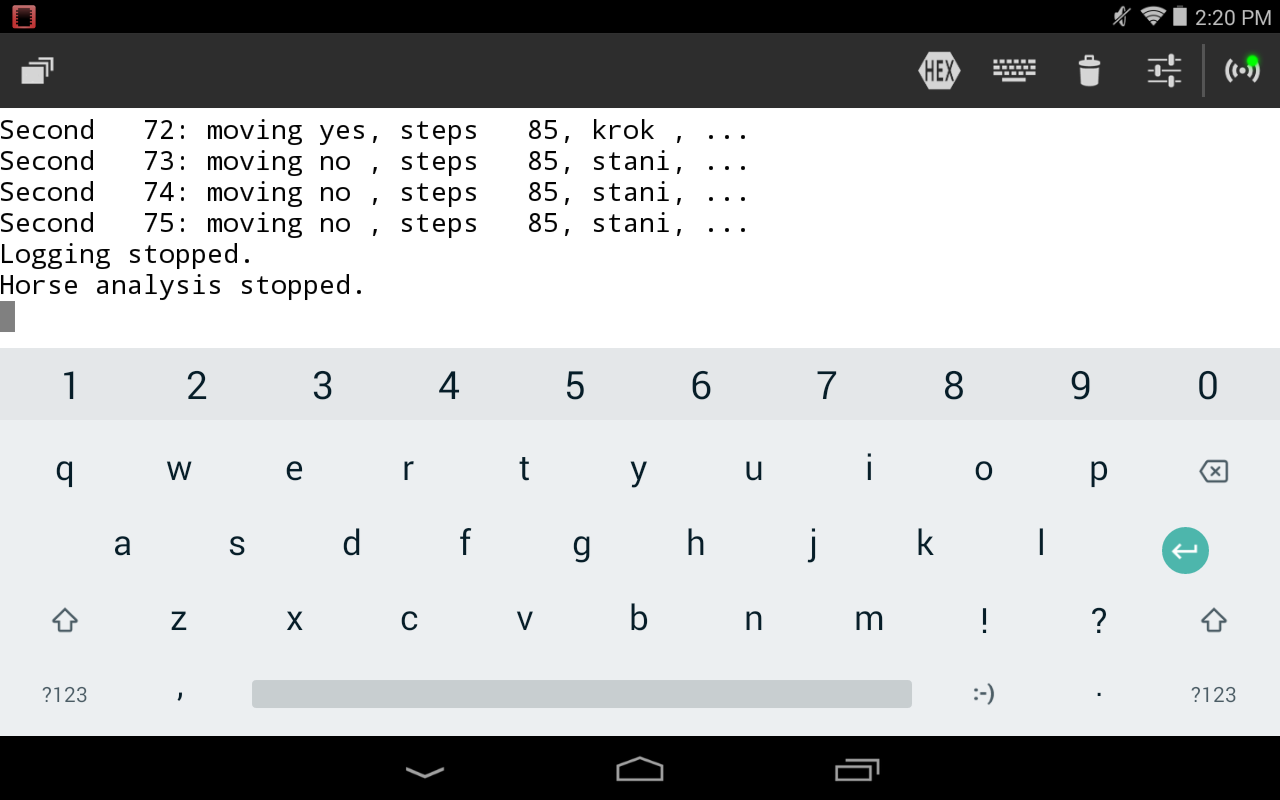
\includegraphics[width=\linewidth]{img/HorseAnalysisTablet.png}
\end{figure}

This tool demonstrates that the SensorBoard is able to run some user code in real-time with real-time results.

\subsection{Controlling via \ac{TCP} connection}
The application can be controlled via \ac{TCP} connection using single letter commands. I recommend implementing a web-page based user interface in the future versions of the application. One letter commands are actually used because it's the easiest way how to control the board from a tablet with on-screen keyboard only. All the communication is possible via the \ac{TCP} connection or via UART through USB connection. The control commands are:

\begin{itemize}
	\item[\textbf{r}] Reset the board and restart the application. We get the same result when we switch the board off and on.
	\item[\textbf{p}] Ping command. When received, the text "Ping received." is printed.
	\item[\textbf{h}] Start/stop the horse movement analysis. When the analysis is running the text output is sent every second.
	\item[\textbf{s}] Start/stop streaming the raw data from the sensors.
	\item[\textbf{l}] Start/stop logging the raw data from the sensors to the SD card. When the logging is in progress, the green software LED is ON on the SensorBoard.
\end{itemize}

\subsection{Using multiple SensorBoards}
When we have more SensorBoards, we can connect them like in figure \ref{UELogging2}. Then all the hardware connected together behaves like one SensorBoard with so many sensors in different places. All the SensorBoards should connect to one WiFi network created by one board or by an external WiFi access point (e.g. mobile phone tethering/hotspot). All the SensorBoards except one (must be configured in the configuration file on SD card) behaves as \ac{TCP} clients and connects to \ac{TCP} server (the last SensorBoard). The \ac{TCP} server resends all the commands to the other boards, so all the SensorBoards behaves synchronously. The log files are stored on the SD card on each board and the names of these files are the same on all connected boards. So, the \ac{TCP} server dictates the names of all log files. One synchronous session creates multiple files on multiple SD cards, but with the same filenames on all devices.

The whole system of connected boards can be used for example like in figure \ref{UELoggingHorse}.

\chapter{Movement Analysis}
- co analyzuju a ceho chci dosahnout!
- umisteni senzoru / senzorů na koni, nakres

\section{Digital Signal Processing}
- pozadavky na data, stejna vzorkovaci frekvence, pouzitelne vysoka frekvence, ...

\section{Types of Analysis}
- prehled jetnotlivych zpusobu analyzy - matematika, selsky rozum, strojove uceni, ...
- analyzy trochu detailneji + obrazky z Matlabu

\subsection{Mathematical Tools}

\subsection{Looking for Structures}
- proc jsem si ji vybral + odkaz na kapitolu Implemented Analysis

\subsection{Machine Learning}

\section{Implemented Analysis}
- popis vybrane analyzy, proc jsem si ji vybral
- to, co jsem posilal v cestine do Monetu

\subsection{Results}
- ukazky mezivysledku na grafech
- vice datovych kanalu, z hlavy, ze sedla, z kopyt
- vysledky analyzy, grafy, data


//todo: ?konverze dat z akcelerometru na zvuk?
\chapter{Conclusion}
The work was finally split into four milestones. The first milestone was achieved when I have decided to develop a new data logging hardware, because the existing solutions didn't fulfilled all the requirements. I have successfully developed the SensorBoard hardware in the second step and then the board was manufactured in six copies. I have achieved the second milestone with the manufactured hardware. The third phase was about testing the hardware and about implementing libraries for communication between the controller and other parts, mainly sensors. I have found several mistakes in the hardware design during programming, but all of them were corrected. The third milestone was achieved when I had a working hardware with C++ libraries for easier communication with sensors and other parts of the hardware. These libraries are a part of the API. During the last phase I have implemented the firmware for real-time movement analysis. When the SensorBoard is placed on a horse under the saddle, it is able to recognize the kind of movement of a horse. This firmware demonstrates the functionality of the designed hardware in real use. I have achieved the last milestone during the first successful test of the platform on a horse's body.

There are many applications and use cases of the SensorBoard presented as examples in the thesis. I have selected the movement analysis case, because this task started the whole project in the begining. The movement analysis firmware shows the advantages of running some user code on the hardware. We can see the results of the analysis in real-time.

If there is an interest on future work with this hardware, I would recommend to create the second version of the SensorBoard with attention to the list of hardware errors presented in this thesis. The SensorBoard was used for example as a simple autopilot of a small quadcopter, so I believe that it will be used in several applications in the near future. I hope that the firmware for the movement analysis of a horse will help to work with this kind of animals easier.

\backmatter

\bibliographystyle{IEEEtran}

% Using file Bibliography.bib
\bibliography{bibliografia}

\appendix
\chapter{Hardware Documentation}
\label{hardwareDocumentation}

\begin{figure}[H]
	\centering
	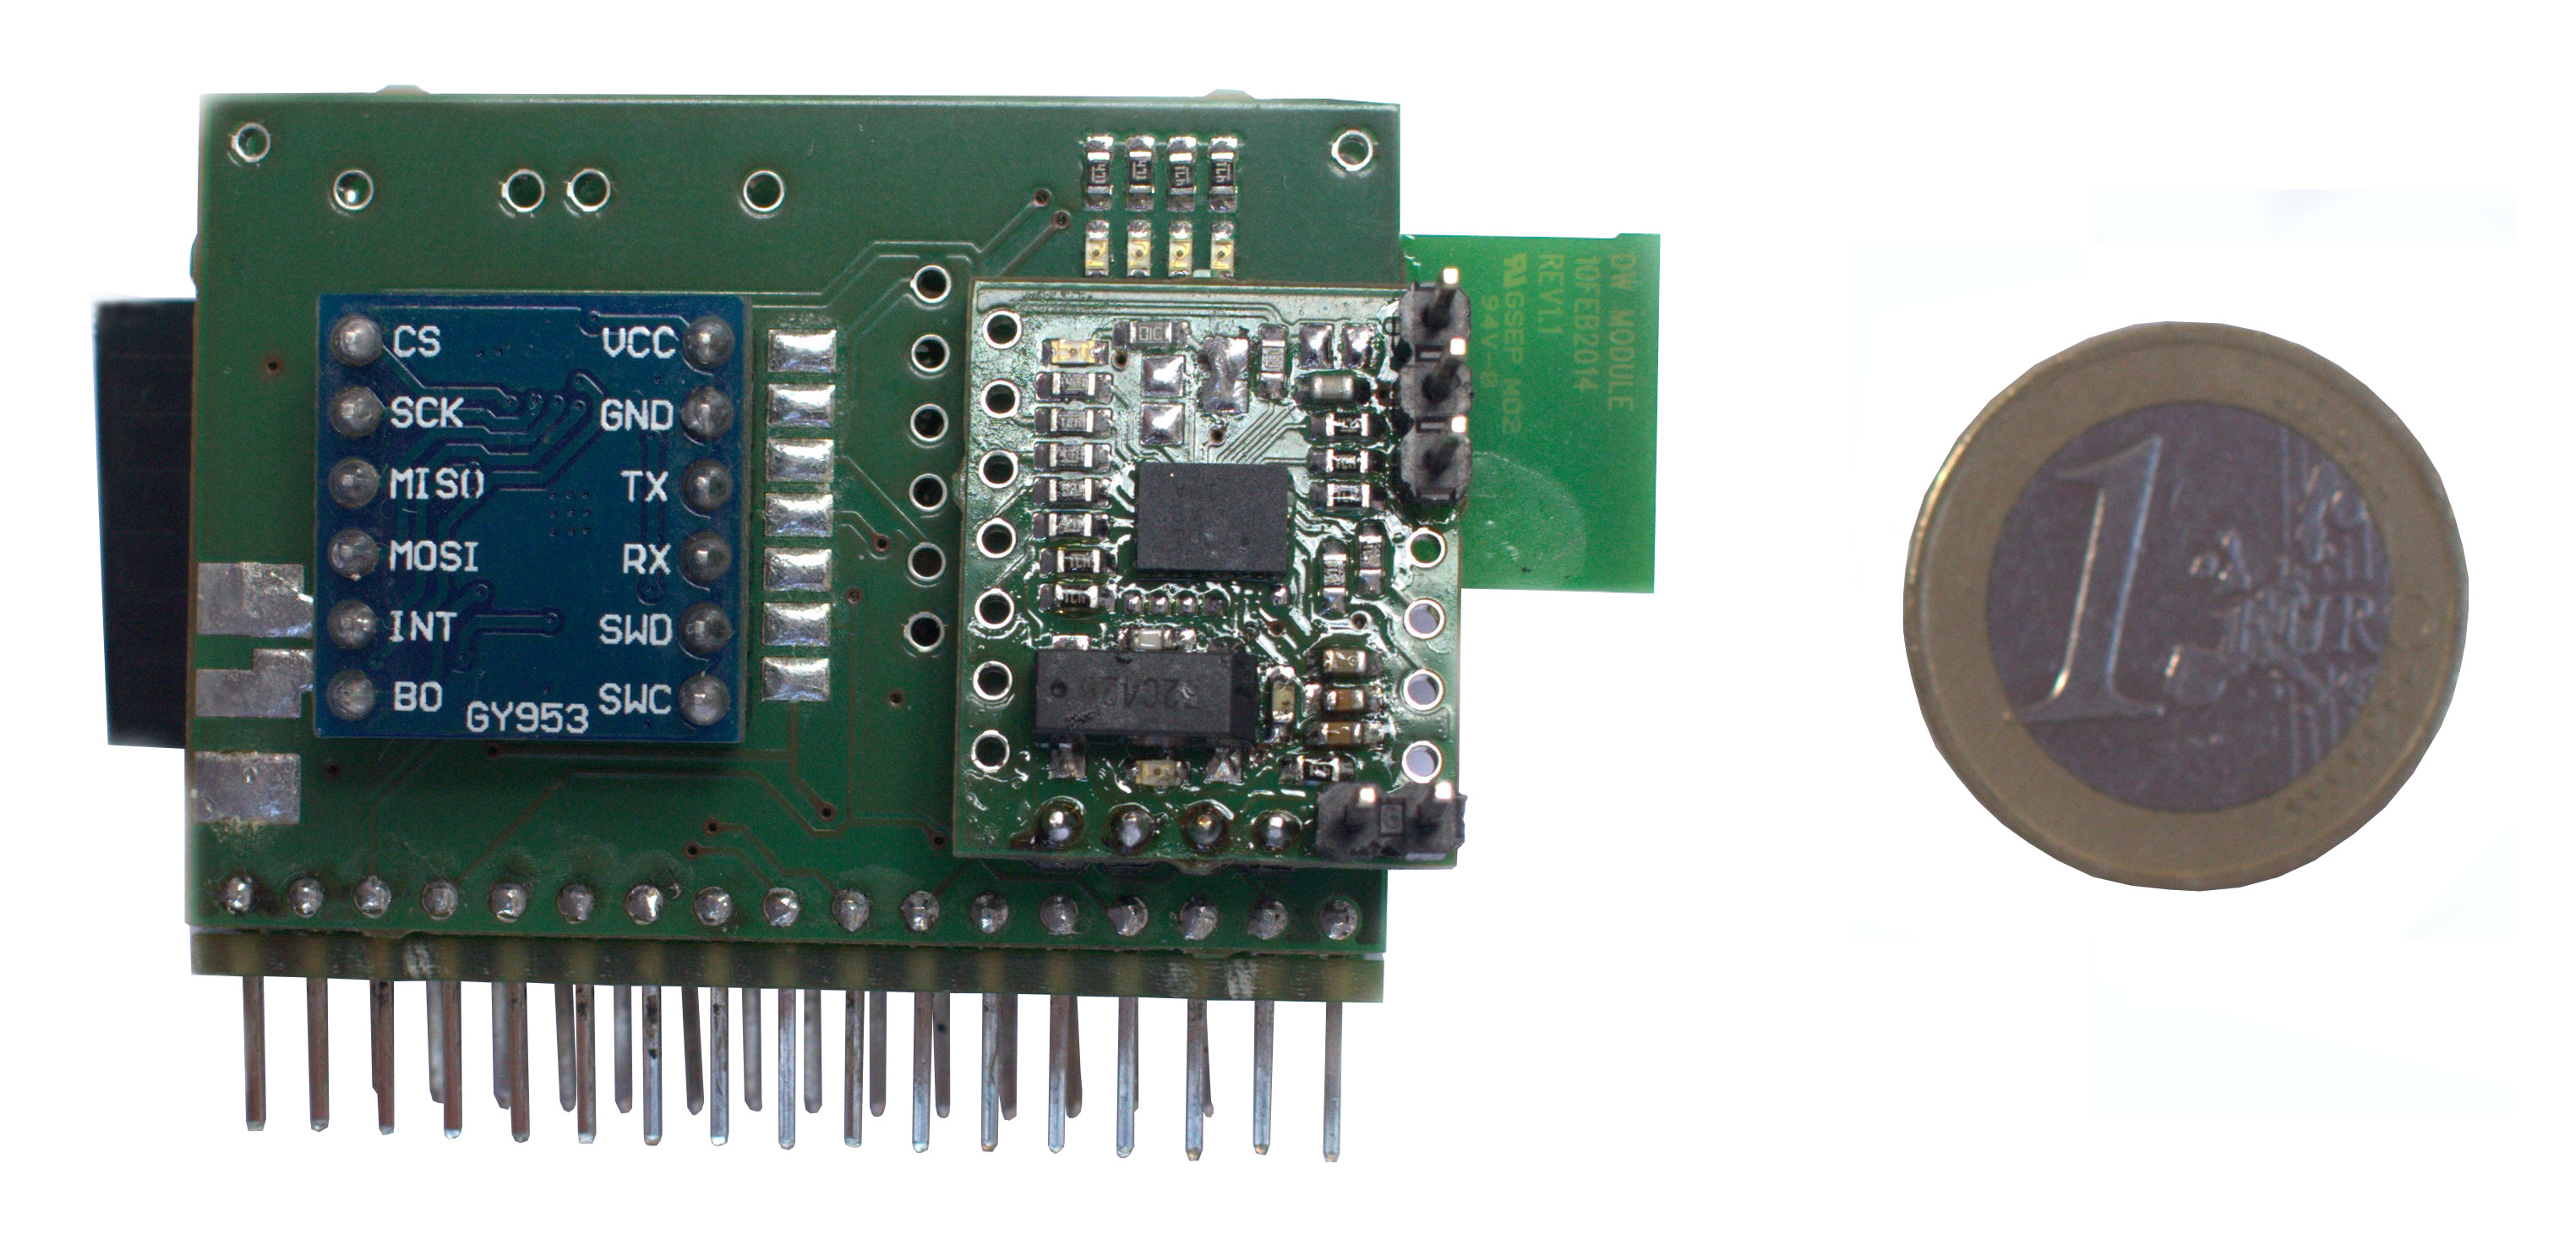
\includegraphics[width=16cm]{img/HWassembled.jpg}
	\label{HWassembled}
	\caption{Assembled Sensor Board prototype}
\end{figure}

\section{Overview}
Sensor Board is a prototype of autonomous hardware platform with microprocessor and various inertial, atmospheric and navigation sensors. The device can be used in many cases from logging data to movement control. The prototype works fully autonomously without connection to external power supply or other electronics, but allows wireless or wired connection to other electronic devices.

\subsection{Features}
\begin{itemize}
	\setlength\itemsep{0.2em}
	\item[--] No external power supply needed
	\item[--] Internal rechargeable battery
	\item[--] Charging from USB or any \SI{5}{V} source
	\item[--] Allowed simultaneous connection to USB and other power supply
	\item[--] Three different triaxial acceleromemers, dynamic gyroscopes and two different triaxial magnetometers
	\item[--] Barometer, light sensor, air humidity, temperature
	\item[--] A/D converters for connecting external sensors
	\item[--] TDOA location system with \SI{10}{cm} precission in \SI{300}{m} radius
	\item[--] External UART connector for GPS or radio communication
	\item[--] Hybrid WiFi and Bluetooth
	\item[--] Servo outputs and connector with other peripheries
	\item[--] User programmable dual core ESP32 processor
	\item[--] Various sleep modes to save battery power
	\item[--] More than 10 hours of operation from battery
	\item[--] Buttons and LEDs for interaction with user
	\item[--] Micro SD card up to \SI{32}{GB} for logging data (accessible from user program)
	\item[--] ARM Cortex-M0 co-processor for computing (sensor fusion, data analysis)
\end{itemize}

\subsection{Properties}

\begin{table}[H]
	\centering
	\begin{tabular}{|l|c|c|}
		\hline
		Parameter & Value & Unit \\
		\hline \hline
		Dimensions & 60 $\cdot$ 31 $\cdot$ 13 & mm \\
		Min Voltage & $-0.5$ & V \\
		Max Voltage & $5.5$ & V \\
		Max current & $2.1$ & A \\
		Max battery life & $12$ & hours \\
		WiFi antenna range & $10$ & m \\
		Bluetooth antenna range & $10$ & m \\
		TDOA location precission & $10$ & cm \\
		TDOA location range & $300$ & m \\
		Average charging time & $60$ & minutes \\
		Min temperature & $-10$ & \degree C \\
		Max temperature & $80$ & \degree C \\
		\hline
	\end{tabular}
	\caption{Properties}
	\label{HWmaxRatings}
\end{table}

\subsection{Power Supply}
//todo: baterka, USB, 5V nezavisle

\section{Getting Started}

\subsection{Assembling}
The device is assembled from three parts, two sandwich boards and one connector board. Optional devices like BMF055 board, GY953, HM-TRP or GPS can be connected to prepared ports. The parts are shown in figure \ref{HWassembling}.

\begin{figure}[H]
	\centering
	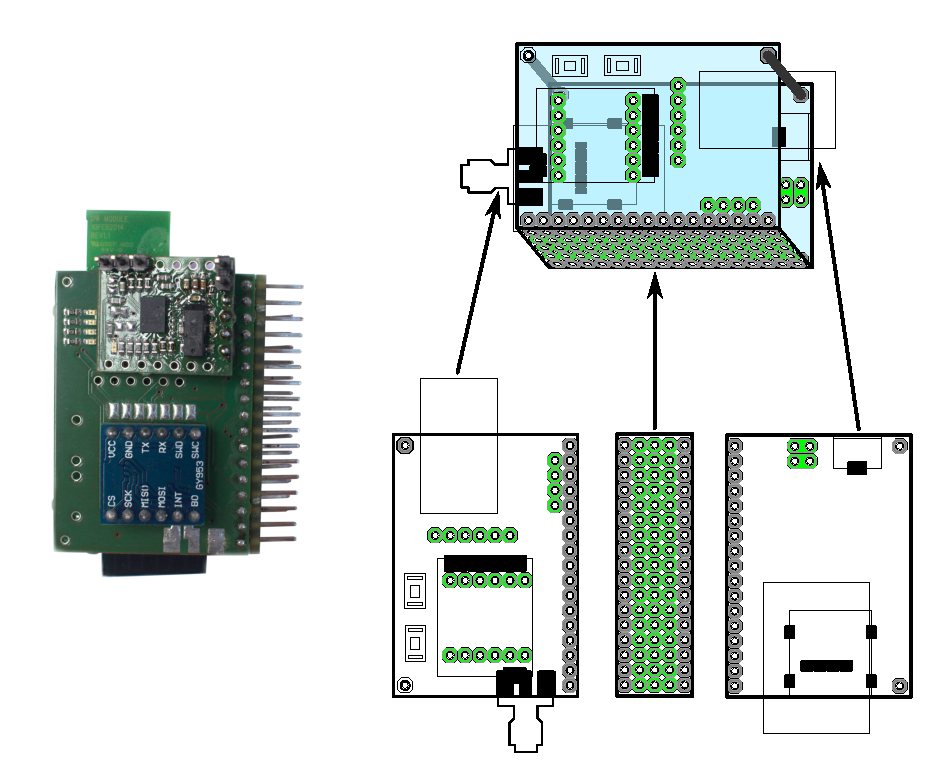
\includegraphics[scale=1]{img/assemblingHW.pdf}
	\label{HWassembling}
	\caption{Assembling the Sensor Board prototype}
\end{figure}

\subsection{Components Description}

\begin{figure}[H]
	\centering
	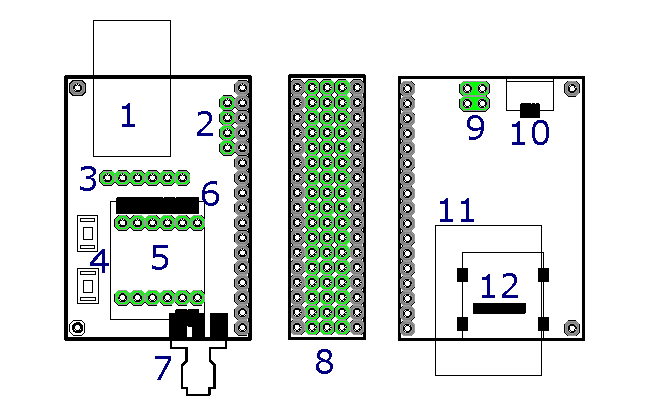
\includegraphics[scale=1]{img/componentsDescription.pdf}
	\label{HWcomponents}
	\caption{Components of the Sensor Board}
\end{figure}

\begin{table}[H]
	\centering
	\begin{tabular}{|c|l|c|}
		\hline
		Number & Description & Datasheet\\
		\hline \hline
		1 & DWM1000 location sensor & //todo \\
		2 & BMF055 board connector (UART) & //todo \\
		3 & HM-TRP 433/868 MHz radio connector & //todo \\
		4 & Software buttons & N/A \\
		5 & GY-953 connector & //todo \\
		6 & HM-TRP 433/868 MHz radio SMD pads & //todo \\
		7 & RPSMA antenna connector for HM-TRP radio & //todo \\
		8 & External pins & Section \ref{pinNumbering} \\
		9 & Battery connector & Section \ref{pinNumbering} \\
		10 & Micro USB connector & //todo \\
		11 & ESP-WROOM-32 with WiFi/Bluetooth antenna & //todo \\
		12 & Micro SD card slot & //todo \\
		\hline
	\end{tabular}
	\caption{Description of components of the Sensor Board}
	\label{table:componentsDescription}
\end{table}

\section{Pin Connections}

\subsection{Pin Numbering}
\label{pinNumbering}

\begin{figure}[H]
	\centering
	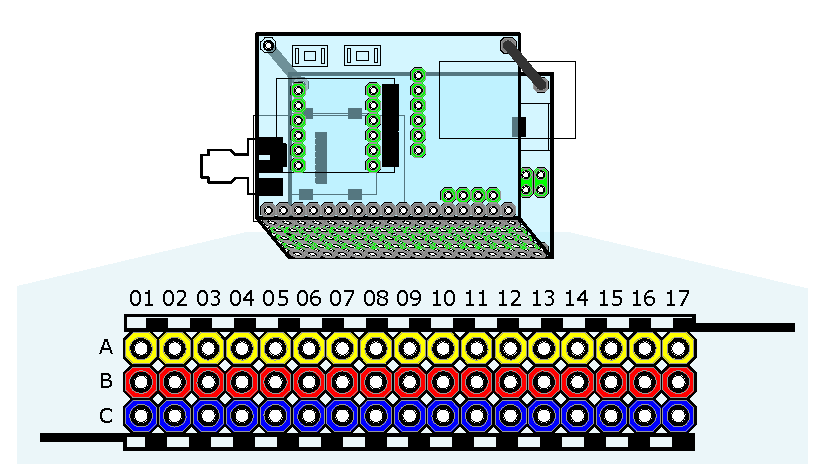
\includegraphics[scale=1]{img/externalPins.pdf}
	\caption{External pins numbering}
	\label{fig:externalPins}
\end{figure}

\begin{table}[H]
	\centering
	\begin{tabular}{|c||c|c|c|c|c|c|c|c|}
		\hline
		& 01 & 02 & 03 & 04 & 05 & 06 & 07 & 08 \\
		\hline \hline
		A & GND & +3V3 & SENSOR\_VP & SENSOR\_VN & IO33 & IO25 & IO32 & IO26 \\
		B & \multicolumn{8}{|c|}{Pins B01 -- B17 internally connected, details in section \ref{jumpersExternalPins}} \\
		C & \multicolumn{8}{|c|}{GND} \\
		\hline
	\end{tabular}

	\vspace{0.5cm}
	
	\begin{tabular}{|c||c|c|c|c|c|c|c|c|c|c|}
		\hline
		& 09 & 10 & 11 & 12 & 13 & 14 & 15 & 16 & 17 & \\
		\hline \hline
		A & IO18 & IO19 & IO21 & IO16 & IO17 & IO23 & IO22 & IO27 & +5V & \\
		B & \multicolumn{10}{|c|}{Pins B01 -- B17 internally connected, details in section \ref{jumpersExternalPins}} \\
		C & \multicolumn{10}{|c|}{GND} \\
		\hline
	\end{tabular}
	\caption{External pins mapping}
	\label{tab:externalPins}
\end{table}

\begin{table}[H]
	\centering
	\begin{tabular}{|c|c|c|c|c|c|}
		\hline
		Number & Name & Safety resistor & Pull-up & Device & Pin \\
		\hline \hline
		01 & GND & N/A & N/A & N/A & N/A \\
		02 & +3V3 & N/A & N/A & N/A & N/A \\
		03 & RADIO\_RX & Yes & No & ESP32 & SENSOR\_VP \\
		04 & RADIO\_TX & Yes & No & ESP32 & SENSOR\_VN \\
		05 & BTN1 & No & Yes & ESP32 & IO33 \\
		06 & BTN0 & No & Yes & ESP32 & IO25 \\
		07 & LED4 & Yes & No & ESP32 & IO32 \\
		08 & SCL0 & Yes & Yes & ESP32 & IO26 \\
		09 & SCK0 & Yes & No & ESP32 & IO18 \\
		10 & MISO0 & Yes & No & ESP32 & IO19 \\
		11 & MOSI0 & Yes & No & ESP32 & IO21 \\
		12 & MPU\_TX & Yes & No & ESP32 & IO16 \\
		13 & MPU\_RX & Yes & No & ESP32 & IO17 \\
		14 & CS\_DECA & Yes & No & ESP32 & IO23 \\
		15 & CS\_MPU2 & Yes & No & ESP32 & IO22 \\
		16 & SDA0 & Yes & No & ESP32 & IO27 \\
		17 & +5V & N/A & N/A & N/A & N/A \\
		\hline
	\end{tabular}
	\caption{External pins properties}
	\label{tab:externalPinsProperties}
\end{table}

\paragraph{Note:} Some external pins are not connected only to processor, but they are connected to other chips in parallel. The other chips are connected only via input only pins or with safety resistor. So, the possibility of damage by incorrect connection or by wrong software is minimized.

\subsection{Pin Description}
\begin{itemize}
	\item 01 -- \textbf{GND}: Ground
	\item 02 -- \textbf{+3V3}: Power Supply \SI{+3.3}{V} from linear stabilizer
	\item 03 -- \textbf{RADIO\_RX}: UART receive pin for external devices like radio communication or GPS
	\item 04 -- \textbf{RADIO\_TX}: UART transmit pin for external devices like radio communication or GPS
	\item 05 -- \textbf{BTN1}: Usage defined by user software, internally connected to button 1
	\item 06 -- \textbf{BTN0}: Usage defined by user software, internally connected to button 0
	\item 07 -- \textbf{LED4}: Usage defined by user software, internally connected to LED4
	\item 08 -- \textbf{SCL0}: \itwoc clock pin for external devices, internally connected to sensors
	\item 09 -- \textbf{SCK0}: SPI clock pin for external devices, internally connected to sensors
	\item 10 -- \textbf{MISO0}: SPI data output pin for external devices, internally connected to sensors
	\item 11 -- \textbf{MOSI0}: SPI data input pin for external devices, internally connected to sensors
	\item 12 -- \textbf{MPU\_TX}: UART transmit pin for GY953 or external device
	\item 13 -- \textbf{MPU\_RX}: UART receive pin for GY953 or external device
	\item 14 -- \textbf{CS\_DECA}: Usage defined by user software, internally used as chip select pin for DWM1000 TDOA location sensor
	\item 15 -- \textbf{CS\_MPU2}: Usage defined by user software, internally connected to GY953 port
	\item 16 -- \textbf{SDA0}: \itwoc data pin for external devices, internally connected to sensors
	\item 17 -- \textbf{+5V}: \SI{+5}{V} power supply from battery or USB or external source, the battery voltage is converted to \SI{5}{V}
\end{itemize}

\paragraph{Note:} All pins except power supply pins can be redefined by software. Their new definition shouldn't be in collision with other connected parts. For details see figures \ref{sch1} and \ref{sch2}.

\subsection{Power Supply}
\label{jumpersExternalPins}
The pins B01 -- B17 are defined by jumpers. We usually need these pins connected to power supply. We can define the voltage by connecting arbitrary B pin to target power supply. The pins B01 -- B17 are internally connected, but they are not connected to anything else. We can define pins B01 -- 17 as:
\begin{itemize}
	\item \textbf{GND} by connecting A01 and B01 by jumper
	\item \textbf{+3V3} by connecting A02 and B02 by jumper
	\item \textbf{+5V} by connecting A17 and B17 by jumper
	\item \textbf{anything} by connecting any B pin to our target
\end{itemize}

\begin{figure}[H]
	\centering
	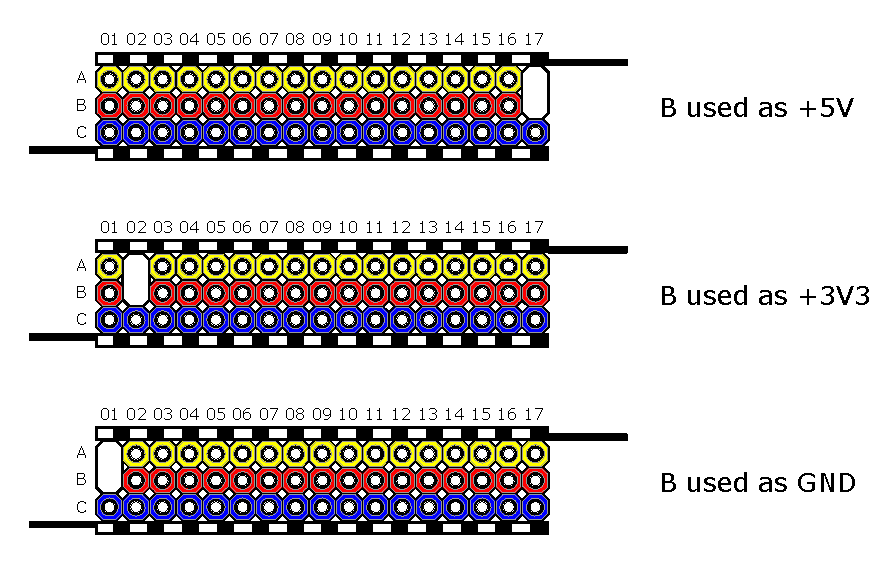
\includegraphics[scale=1]{img/jumpers.pdf}
	\caption{Power supply definition by jumpers}
	\label{fig:jumpersSupply}
\end{figure}

\section{LED Meanings}

\begin{figure}[H]
	\centering
	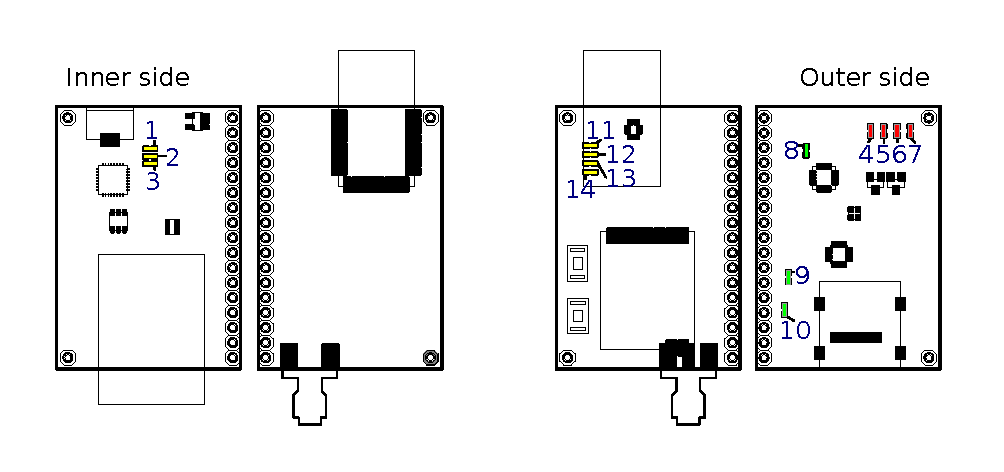
\includegraphics[scale=1]{img/LEDmeanings.pdf}
	\caption{Sensor Board LED meanings}
	\label{fig:LEDmeaning}
\end{figure}

\begin{enumerate}
	\item \textbf{LED\_CBUS3}: (yellow) FTDI LED \cite{FTDI}, USB power indication
	\item \textbf{LED\_CBUS2}: (yellow) FTDI LED \cite{FTDI}, USB connection indication
	\item \textbf{LED\_CBUS4}: (yellow) FTDI LED \cite{FTDI}, USB data transfer indication
	\item \textbf{LED\_5V}: (red) \SI{5}{V} power LED
	\item \textbf{LED\_3V3}: (red) \SI{3.3}{V} power LED
	\item \textbf{LED\_VCCIO}: (red) VCCIO power LED
	\item \textbf{LED\_USB}: (red) USB power LED
	\item \textbf{LED6}: (green) Charging the battery indication
	\item \textbf{LED4}: (green) Software configurable LED
	\item \textbf{LED5}: (green) Software configurable LED
	\item \textbf{LED7}: (yellow) DWM1000 TXLED \cite{DWM1000}
	\item \textbf{LED3}: (yellow) DWM1000 RXLED \cite{DWM1000}
	\item \textbf{LED2}: (yellow) DWM1000 SFDLED \cite{DWM1000}
	\item \textbf{LED1}: (yellow) DWM1000 RXOKLED \cite{DWM1000}
\end{enumerate}

\section{Internal Connections}

\subsection{Internal Pins}
//todo

\begin{figure}[H]
	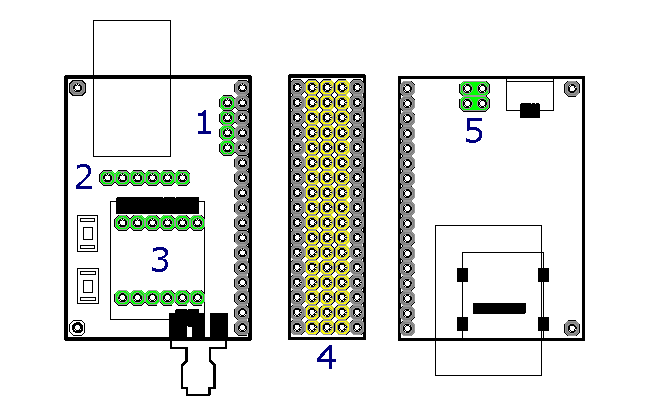
\includegraphics[scale=1]{img/pinSections.pdf}
\end{figure}

\begin{table}[H]
	\begin{tabular}{|c|c|l|}
		\hline
		Number & Usage & Description \\
		\hline
		1 & Internal & BMF055 board connector (UART) \\
		2 & Internal & HM-TRP 433/868 MHz radio connector \\
		3 & Internal & GY-953 connector \\
		4 & External & External pins \\
		5 & Internal & Battery connector \\
		\hline
	\end{tabular}
\end{table}

//todo: detaily ke kazdemu

\subsubsection{BMF055 board connector (UART)}
\subsubsection{HM-TRP 433/868 MHz radio connector}
\subsubsection{GY-953 connector}
\subsubsection{External pins} \ref{pinNumbering}
\subsubsection{Battery connector}

//todo: vyznam testpadu

\section{BMF055 Extension Board}
\label{BMF055pinNumbering}
//todo

\subsection{Pin Connection}
//todo

\subsection{LED Meanings}
//todo



\section{Sensor Board Drawings}
//todo: pridat vedle sebe fotku, render, nakres a eagle brd


\end{document}
